% !TEX program = pdflatex
% ============================================================
% SKILLNAV - Rapport methodologique final
% Module M242 Analyse de Web - ENSA Tetouan - SDBIA
% Auteurs : Bachirou Konate & Karamo Sylla
% Encadrant : Pr. Imad Sassi
% Annee universitaire 2025-2026
% ============================================================

\documentclass[11pt,a4paper,openany]{report}

% ----- Encodage et langue (pdfLaTeX) -----
\usepackage[utf8]{inputenc}
\usepackage[T1]{fontenc}
\usepackage[french]{babel}

% ----- Polices Latin Modern (par defaut pdfLaTeX) -----
\usepackage{lmodern}
\usepackage{microtype}
% \headingfont = sans-serif (alias compatible avec le code existant)
\newcommand{\headingfont}{\sffamily}

% ----- Geometrie page -----
\usepackage[a4paper,top=2.5cm,bottom=2.5cm,left=2.5cm,right=2.5cm]{geometry}

% ----- Couleurs charte -----
\usepackage{xcolor}
\definecolor{navy}{HTML}{0A2540}
\definecolor{royalblue}{HTML}{1E5BFF}
\definecolor{softblue}{HTML}{E6EEFB}
\definecolor{accent}{HTML}{1FB387}
\definecolor{lightgray}{HTML}{F5F7FB}
\definecolor{mediumgray}{HTML}{6C7A89}

% ----- Tableaux -----
\usepackage{booktabs}
\usepackage{array}
\usepackage{tabularx}
\usepackage{longtable}
\usepackage{multirow}
\usepackage{colortbl}
\usepackage{ragged2e}
\newcolumntype{L}[1]{>{\RaggedRight\arraybackslash}p{#1}}
\newcolumntype{C}[1]{>{\Centering\arraybackslash}p{#1}}
\newcolumntype{R}[1]{>{\RaggedLeft\arraybackslash}p{#1}}
\renewcommand{\arraystretch}{1.25}

% ----- Figures -----
\usepackage{graphicx}
\graphicspath{{IMAGES_RAPPORT/}{./IMAGES_RAPPORT/}}
\usepackage{float}
\usepackage{subcaption}
\usepackage{caption}
\captionsetup{
  font={small},
  labelfont={bf,color=navy},
  textfont={it},
  labelsep=period,
  justification=centering
}

% ----- Code (listings) -----
\usepackage{listings}
\lstdefinelanguage{pythonlike}{
  morekeywords={class,def,return,for,in,if,else,elif,True,False,None,from,import,as,with,not,and,or,is,lambda,pass,raise,try,except,finally},
  morecomment=[l]{\#},
  morestring=[b]",
  morestring=[b]',
}
\lstset{
  basicstyle=\ttfamily\footnotesize\color{navy!90!black},
  backgroundcolor=\color{lightgray},
  frame=single,
  framerule=0pt,
  rulecolor=\color{lightgray},
  xleftmargin=10pt,
  xrightmargin=10pt,
  framesep=8pt,
  breaklines=true,
  breakatwhitespace=true,
  showstringspaces=false,
  columns=fullflexible,
  keywordstyle=\color{royalblue}\bfseries,
  commentstyle=\color{mediumgray}\itshape,
  stringstyle=\color{accent},
  numbers=left,
  numberstyle=\tiny\color{mediumgray},
  numbersep=8pt,
  captionpos=b,
  language=pythonlike,
  literate=
    {é}{{\'e}}1 {è}{{\`e}}1 {ê}{{\^e}}1 {ë}{{\¨e}}1
    {à}{{\`a}}1 {â}{{\^a}}1
    {î}{{\^\i}}1 {ï}{{\¨\i}}1
    {ô}{{\^o}}1 {ö}{{\¨o}}1
    {ù}{{\`u}}1 {û}{{\^u}}1
    {ç}{{\c c}}1
    {É}{{\'E}}1 {È}{{\`E}}1 {Ê}{{\^E}}1
    {À}{{\`A}}1 {Â}{{\^A}}1
    {Î}{{\^I}}1 {Ô}{{\^O}}1 {Ù}{{\`U}}1 {Û}{{\^U}}1
    {Ç}{{\c C}}1
}

% ----- Hyperliens -----
\usepackage[hidelinks]{hyperref}
\hypersetup{
  pdftitle  = {SKILLNAV - Observatoire des competences IA et Data Science},
  pdfauthor = {Bachirou Konate, Karamo Sylla},
  pdfsubject= {Rapport methodologique - M242 Analyse de Web - ENSA Tetouan},
  colorlinks=true,
  linkcolor =navy,
  urlcolor  =royalblue,
  citecolor =navy
}

% ----- Style des titres -----
\usepackage{titlesec}
\titleformat{\chapter}[display]
  {\headingfont\color{navy}\bfseries}
  {\filright\Large\MakeUppercase{\chaptertitlename}~\thechapter}
  {1ex}
  {\titlerule[1pt]\vspace{0.8ex}\filright\Huge}
\titlespacing*{\chapter}{0pt}{0pt}{30pt}

\titleformat{\section}
  {\headingfont\color{navy}\Large\bfseries}
  {\thesection}{1em}{}
\titleformat{\subsection}
  {\headingfont\color{royalblue}\large\bfseries}
  {\thesubsection}{0.8em}{}
\titleformat{\subsubsection}
  {\headingfont\normalsize\bfseries\color{navy!85!black}}
  {\thesubsubsection}{0.7em}{}

% ----- En-tetes et pieds -----
\usepackage{fancyhdr}
\pagestyle{fancy}
\fancyhf{}
\renewcommand{\headrulewidth}{0pt}
\fancyfoot[C]{\textcolor{mediumgray}{\small\thepage}}
\fancyhead[L]{\textcolor{mediumgray}{\small\leftmark}}
\fancyhead[R]{\textcolor{mediumgray}{\small SKILLNAV}}
\renewcommand{\headrulewidth}{0.3pt}
\renewcommand{\footrulewidth}{0pt}

% ----- Espacements et listes -----
\setlength{\parindent}{0pt}
\setlength{\parskip}{0.55em}
\renewcommand{\baselinestretch}{1.18}
\usepackage{enumitem}
\setlist{itemsep=2pt, topsep=4pt, parsep=0pt}

% ----- Commandes personnelles -----
\usepackage{xspace}
\newcommand{\skillnav}{\textsc{SkillNav}\xspace}

% ============================================================
\begin{document}

% =============== PAGE DE GARDE ==============================
\begin{titlepage}
  \noindent\textcolor{navy}{\rule{\textwidth}{6pt}}
  \centering
  \vspace*{1cm}

  
\includegraphics[width=0.32\textwidth]{logo_ensa.png}\\[1.2cm]

  {\headingfont\color{navy}\large\bfseries
   \'Ecole Nationale des Sciences Appliqu\'ees de T\'etouan}\\[0.25cm]
  {\color{mediumgray}\itshape Universit\'e Abdelmalek Essa\^adi}\\[0.4cm]

  \rule{0.6\textwidth}{0.4pt}\\[0.4cm]
  {\headingfont\large\bfseries Cycle d'ing\'enieur}\\[0.2cm]
  {\color{navy}\large Fili\`ere SDBIA - Sciences des Donn\'ees, Big Data et Intelligence Artificielle}\\[0.15cm]
  {\color{mediumgray}\small Module M242 - Analyse de Web}\\[1.6cm]

  {\headingfont\color{navy}\fontsize{36pt}{42pt}\selectfont\bfseries SKILLNAV}\\[0.35cm]
  {\headingfont\color{royalblue}\Large\itshape Observatoire des comp\'etences\\
   en Intelligence Artificielle et Data Science\\
   par Web Mining}\\[0.6cm]
  \rule{0.45\textwidth}{0.5pt}\\[0.4cm]
  {\large Rapport m\'ethodologique final}\\[2cm]

  \begin{minipage}[t]{0.48\textwidth}
    \raggedright
    \textbf{\color{navy}R\'ealis\'e par :}\\[0.15cm]
    Bachirou \textsc{Konat\'e}\\
    Karamo \textsc{Sylla}
  \end{minipage}\hfill
  \begin{minipage}[t]{0.48\textwidth}
    \raggedleft
    \textbf{\color{navy}Encadr\'e par :}\\[0.15cm]
    Pr. Imad \textsc{Sassi}
  \end{minipage}\\[2.5cm]

  {\large\headingfont\color{navy}Ann\'ee universitaire 2025-2026}\\[0.2cm]
  {\small\color{mediumgray}Soutenance pr\'evue le 28 mai 2026}

  \vfill
  \noindent\textcolor{royalblue}{\rule{\textwidth}{3pt}}
\end{titlepage}

% =============== FRONTMATTER ================================
\pagenumbering{roman}
\setcounter{tocdepth}{2}

{\hypersetup{linkcolor=navy}
  \tableofcontents
}
\clearpage

\listoffigures
\clearpage

\listoftables
\clearpage

\pagenumbering{arabic}

% =============== CHAPITRE 1 =================================
\chapter{Introduction et vue d'ensemble}

\section{Contexte du projet}

Le march\'e des comp\'etences en Intelligence Artificielle et en Data Science a connu, depuis la sortie publique de ChatGPT en novembre 2022, une transformation structurelle d'une rapidit\'e et d'une ampleur in\'edites dans l'histoire r\'ecente du march\'e du travail tertiaire. Le World Economic Forum a estim\'e dans son rapport \emph{Future of Jobs} 2025 que les comp\'etences en Intelligence Artificielle figurent d\'esormais parmi les cinq comp\'etences techniques dont la demande cro\^it le plus rapidement \`a l'\'echelle mondiale, devant la cybers\'ecurit\'e et le d\'eveloppement logiciel g\'en\'eraliste (World Economic Forum, 2025). L'Organisation de Coop\'eration et de D\'eveloppement \'Economiques (OECD) a document\'e un d\'eplacement de la demande des employeurs vers des profils ma\^itrisant \`a la fois les fondamentaux du Machine Learning classique et les techniques propres \`a l'Intelligence Artificielle g\'en\'erative, en particulier les mod\`eles de langage de grande taille, l'ing\'enierie de prompts et les architectures de g\'en\'eration augment\'ee par r\'ecup\'eration (OECD, 2024).

Cette transformation rapide pose une question structurelle aux institutions de formation. Le rythme d'\'evolution du march\'e d\'epasse celui des cycles de r\'evision des maquettes p\'edagogiques, en particulier dans les pays o\`u les programmes d'ing\'enieur sont r\'eglement\'es par tutelle minist\'erielle. Au Maroc, le r\'eseau public des \'Ecoles Nationales des Sciences Appliqu\'ees compte douze \'etablissements, dont huit dispensent une fili\`ere Data Science, Big Data ou Intelligence Artificielle en cycle ing\'enieur. La question implicite \`a laquelle le pr\'esent projet apporte une r\'eponse empirique est la suivante : dans quelle mesure les fili\`eres actuelles pr\'eparent-elles les dipl\^om\'es au march\'e effectivement observable des emplois en Intelligence Artificielle et en Data Science ? La r\'eponse \`a cette question suppose au pr\'ealable une connaissance fine et chiffr\'ee du march\'e, dont la construction constitue le c\oe ur du pr\'esent rapport. Le rapprochement entre les comp\'etences enseign\'ees et les comp\'etences demand\'ees est conduit au chapitre 5.1.

\section{Probl\'ematique et objectifs}

Le projet \skillnav s'organise autour de trois questions de recherche, chacune correspondant \`a un axe canonique du Web Mining tel que d\'efini par Liu (2011).

\begin{itemize}
  \item La premi\`ere question, \textbf{Q1 (Content Mining)}, porte sur l'extraction automatique et fiable des comp\'etences techniques mentionn\'ees dans les offres d'emploi publi\'ees sur le web. Cette question se d\'ecline en deux sous-questions op\'erationnelles : quel mod\`ele de reconnaissance d'entit\'es nomm\'ees maximise le score F1 sur un corpus multilingue mixte fran\c{c}ais et anglais, et \`a quel co\^ut computationnel ?
  \item La deuxi\`eme question, \textbf{Q2 (Structure Mining)}, porte sur l'organisation des comp\'etences extraites en familles coh\'erentes et sur l'identification des comp\'etences pivot. Elle se d\'ecline en : quelles structures communautaires \'emergent du graphe de co-occurrence des comp\'etences, et quelle est la coh\'erence s\'emantique de ces communaut\'es ?
  \item La troisi\`eme question, \textbf{Q3 (Usage Mining)}, porte sur l'anticipation de l'\'evolution des comp\'etences en demande \`a un horizon court (quatre \`a douze semaines). Elle se d\'ecline en : quel mod\`ele de forecasting offre la meilleure pr\'ecision sur des s\'eries temporelles courtes (de l'ordre de seize semaines exploitables) et quelles comp\'etences sont susceptibles d'\'emerger ou de d\'ecliner sur la fen\^etre de pr\'evision ?
\end{itemize}

\`A ces trois questions principales s'ajoute une \textbf{question d\'eriv\'ee} propre au volet curricula : \'etant donn\'e les comp\'etences effectivement demand\'ees par le march\'e, dans quelle mesure les programmes p\'edagogiques des huit ENSA marocaines proposant une fili\`ere Data ou Intelligence Artificielle pr\'eparent-ils les dipl\^om\'es \`a ce march\'e ? Cette question est trait\'ee au chapitre 5.1 sous la forme d'une analyse comparative (\emph{gap analysis}) entre comp\'etences enseign\'ees et comp\'etences demand\'ees.

\section{Les trois axes du Web Mining}

Le Web Mining, d\'efini par Liu (2011) comme l'application des techniques de fouille de donn\'ees aux ressources accessibles sur le web, se d\'ecompose canoniquement en trois axes compl\'ementaires. Le \textbf{Content Mining} s'int\'eresse \`a l'extraction d'informations structur\'ees \`a partir du contenu textuel des pages, en mobilisant les techniques du traitement automatique du langage naturel et plus r\'ecemment les mod\`eles transformer pr\'e-entra\^in\'es. Le \textbf{Structure Mining} s'int\'eresse \`a la mod\'elisation des relations entre les entit\'es extraites sous forme de graphes, et \`a l'application d'algorithmes d'analyse de r\'eseaux pour faire \'emerger des partitions, des centralit\'es ou des chemins significatifs. L'\textbf{Usage Mining} s'int\'eresse \`a l'analyse des s\'eries temporelles et des trajectoires d'usage, en mobilisant les techniques classiques du forecasting et de la d\'etection d'\'ev\'enements.

Le projet \skillnav se distingue par sa \textbf{couverture \'equilibr\'ee des trois axes} sur un m\^eme domaine applicatif. Cette ambition est exig\'ee par le sujet impos\'e du module M242, qui demande \`a chaque \'equipe de d\'emontrer empiriquement la ma\^itrise des trois axes plut\^ot que de sp\'ecialiser le projet sur un seul d'entre eux. La pond\'eration retenue pour la production du projet est de 35\,\% sur le Content Mining (extraction et NER), 30\,\% sur le Structure Mining (graphe et communaut\'es), 30\,\% sur l'Usage Mining (forecasting), et 5\,\% sur les composants transverses (Data Quality Framework, dashboard, RGPD). Cette r\'epartition garantit un \'equilibre acad\'emique tout en accordant une l\'eg\`ere priorit\'e au Content Mining, dont la qualit\'e conditionne en amont celle des deux autres axes.

\section{Architecture globale du projet}

Le pipeline \skillnav est organis\'e en sept \'etages s\'equentiels, depuis la collecte initiale des offres d'emploi jusqu'\`a leur restitution dans une interface web interactive. La figure~\ref{fig:archi-globale} ci-dessous synth\'etise cette architecture en explicitant, pour chaque \'etage, les outils techniques mobilis\'es et la nature des artefacts produits.

\begin{figure}[H]
  \centering
  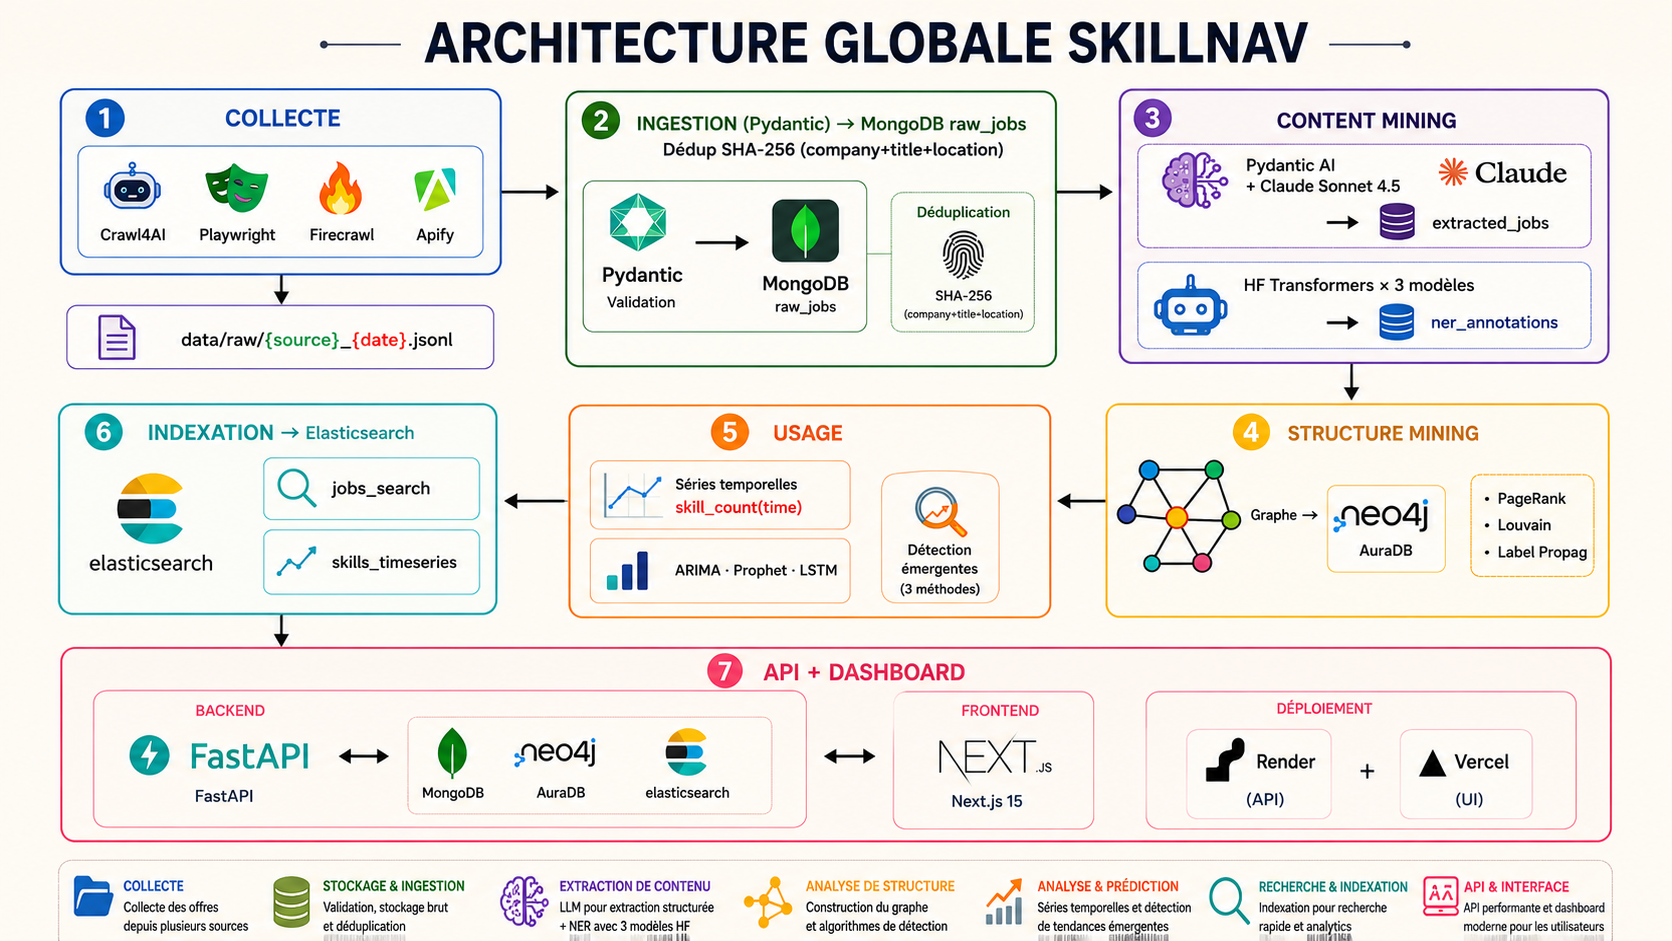
\includegraphics[width=0.85\textwidth]{schema-globale.png}
  \caption{Architecture du pipeline \skillnav en sept \'etages s\'equentiels, de la collecte des offres jusqu'au dashboard utilisateur.}
  \label{fig:archi-globale}
\end{figure}

La stack technique retenue r\'esulte d'arbitrages document\'es en annexe~F sous la forme d'enregistrements de d\'ecisions d'architecture. Le langage Python 3.12 est retenu pour l'ensemble de la cha\^ine d'extraction et d'analyse. La gestion des d\'ependances repose sur Poetry, avec verrouillage strict des versions via \texttt{poetry.lock} commit\'e dans le d\'ep\^ot. Les sch\'emas de donn\'ees sont d\'efinis par les mod\`eles Pydantic v2 et constituent la source de v\'erit\'e unique des conversions vers les trois bases NoSQL. Les mod\`eles d'Intelligence Artificielle sont fournis par Anthropic (Claude Sonnet 4.5 et Haiku 4.5 pour l'extraction structur\'ee) et par Hugging Face Transformers (BERT multilingue, CamemBERT-NER, DistilBERT-NER pour la reconnaissance d'entit\'es nomm\'ees). Les bases de donn\'ees sont h\'eberg\'ees sur trois services cloud distincts en formule gratuite : MongoDB Atlas pour le stockage canonique, Neo4j AuraDB pour le graphe, et OpenSearch via Bonsai pour la recherche. L'interface utilisateur est d\'evelopp\'ee en Next.js 15 avec TypeScript 5.4 et d\'eploy\'ee sur Vercel. L'API est d\'evelopp\'ee en FastAPI et d\'eploy\'ee sur Render.

L'interface utilisateur \skillnav se pr\'esente sous la forme d'un dashboard public en lecture seule, organis\'e en huit pages th\'ematiques : page d'accueil avec indicateurs cl\'es, page Comp\'etences avec tableau filtrable, page Graphe avec rendu interactif, page Forecasting avec superposition des trois mod\`eles, page NER Explorer avec annotation c\^ote \`a c\^ote, page M\'ethodologie, page \'Etude Comparative et page Data Quality. Les captures \'ecran des pages livr\'ees au moment du rendu sont report\'ees en annexe~B.

\section{Chiffres cl\'es du projet}

Le tableau~\ref{tab:chiffres-cles} synth\'etise les indicateurs quantitatifs principaux du projet \`a la date de finalisation du rapport.

\begin{table}[H]
  \centering
  \caption{Chiffres cl\'es du projet \skillnav \`a la date de finalisation du rapport (mai 2026).}
  \label{tab:chiffres-cles}
  \begin{tabularx}{0.95\textwidth}{>{\bfseries\color{navy}}X r}
    \toprule
    \rowcolor{softblue}\textbf{Indicateur} & \textbf{Valeur} \\
    \midrule
    Volume total d'offres collect\'ees & 3\,467 fiches (381 Maroc + 3\,086 International) \\
    P\'eriode d'observation & ao\^ut 2022 \`a mai 2026 \\
    Distribution temporelle des offres & 53 fiches ao\^ut 2022 \`a d\'ecembre 2025 ; 3\,396 fiches janvier \`a mai 2026 \\
    Entreprises distinctes Maroc & 147 \\
    Entreprises distinctes International & 1\,378 \\
    N\oe uds du graphe Neo4j & 8\,934 \\
    Relations du graphe Neo4j & 40\,899 \\
    Index MongoDB Atlas & 17 \\
    Score F1 du meilleur mod\`ele NER & 0,463 (DistilBERT-NER) \\
    Modularit\'e Q du meilleur algorithme de communaut\'es & 0,2988 (Leiden) \\
    RMSE m\'edian du meilleur mod\`ele de forecasting & 17,21 (ARIMA) \\
    \bottomrule
  \end{tabularx}
\end{table}

Plusieurs de ces chiffres m\'eritent un commentaire imm\'ediat. Le volume collect\'e (3\,467 fiches) d\'epasse de 73\,\% la cible haute de 2\,000 fiches initialement fix\'ee pour la version MVP du projet, ce qui assure une assise statistique suffisante pour les analyses comparatives du chapitre~4. La consommation des quotas gratuits des trois bases NoSQL reste tr\`es faible (4\,\% pour Neo4j AuraDB, moins de 2\,\% pour MongoDB Atlas et pour OpenSearch Bonsai), ce qui d\'emontre la viabilit\'e d'un d\'eploiement p\'edagogique sans engagement financier. Le co\^ut total du projet, estim\'e \`a moins de cinquante dollars principalement consomm\'es par les appels \`a l'API Anthropic et \`a l'API Apify pour le scraping LinkedIn, illustre l'accessibilit\'e \'economique d'un observatoire de march\'e construit selon les principes du Web Mining sur infrastructure cloud gratuite.

% =============== CHAPITRE 2 =================================
\chapter{M\'ethodologie}

Le pr\'esent chapitre expose la m\'ethodologie compl\`ete mise en \oe uvre dans le projet \skillnav, depuis la strat\'egie de collecte des donn\'ees jusqu'aux pipelines analytiques des trois axes du Web Mining, en passant par l'architecture des bases de donn\'ees NoSQL et le cadre de conformit\'e r\'eglementaire. Chaque section pr\'esente d'abord les principes m\'ethodologiques retenus, justifie ensuite les choix techniques effectu\'es, puis d\'etaille les param\`etres d'impl\'ementation qui rendent les r\'esultats reproductibles. Les choix d'architecture sont \'etay\'es par les enregistrements de d\'ecisions report\'es en annexe~F.

\section{Collecte de donn\'ees}

\subsection{P\'erim\`etre m\'etiers et g\'eographique}

Le p\'erim\`etre m\'etiers du projet est strictement d\'elimit\'e au champ \textbf{Data Science et Intelligence Artificielle}. Sont inclus dans la collecte les intitul\'es correspondant aux profils suivants : Data Analyst, Business Analyst, Business Intelligence Analyst, Data Scientist, Data Engineer, Machine Learning Engineer, MLOps Engineer, AI Engineer, NLP Engineer, Computer Vision Engineer, Generative AI Engineer, Large Language Model Engineer, Data Architect, Research Scientist en donn\'ees, et Quantitative Engineer impliquant du Machine Learning. Sont express\'ement exclus les profils transverses du d\'eveloppement logiciel (Full Stack Developer, Software Developer g\'en\'eraliste, DevOps Engineer sans dimension Machine Learning), de la cybers\'ecurit\'e sans composante data, du management de projet informatique, et du support technique. Les cas fronti\`ere (par exemple Business Intelligence Analyst Power Platform) sont admis si la description mentionne explicitement une dimension pr\'edictive ou analytique avanc\'ee.

Le p\'erim\`etre g\'eographique privil\'egie le Maroc en source primaire et compl\`ete la collecte par des sources internationales destin\'ees \`a servir de r\'ef\'erence comparative. La p\'eriode d'observation s'\'etend d'ao\^ut 2022 \`a mai 2026, ancr\'ee sur la sortie publique de ChatGPT en novembre 2022 consid\'er\'ee comme \'ev\'enement structurant du march\'e des comp\'etences en Intelligence Artificielle.

\subsection{Strat\'egie multi-sources}

Sept sources distinctes ont \'et\'e retenues \`a l'issue d'une cartographie pr\'ealable des plateformes d'annonces d'emploi accessibles au public. Le d\'etail des sources, des volumes collect\'es et des m\'ethodes de collecte est pr\'esent\'e dans le tableau~\ref{tab:sources-collecte}.

\begin{table}[H]
  \centering
  \caption{Distribution des sources collect\'ees dans le projet \skillnav avec volumes, m\'ethodes et niveau de priorit\'e.}
  \label{tab:sources-collecte}
  \small
  \begin{tabularx}{\textwidth}{l L{2.6cm} r L{4.5cm} c}
    \toprule
    \rowcolor{softblue}\textbf{Origine} & \textbf{Source} & \textbf{Volume} & \textbf{M\'ethode de collecte} & \textbf{Tier} \\
    \midrule
    Maroc & ANAPEC & 2 & Playwright (HTML statique) & T1 \\
    Maroc & Rekrute & 27 & Playwright + Wayback Machine & T1 \\
    Maroc & Indeed Maroc & 67 & Apify actor + recovery & T1 \\
    Maroc & LinkedIn Maroc & 207 & Apify \texttt{cheap-advance-linkedin-jobs-scraper} & T1 \\
    Maroc & Pages carri\`eres employeurs & 6 & Firecrawl + extraction JSON-LD & T1 \\
    Maroc & Glassdoor Maroc & 72 & Firecrawl + recovery & T1 \\
    International & Corpus Tech INTL (builtin.com) & 3\,086 & Pipeline cinq \'etapes (import upstream) & T1 \\
    \midrule
    \rowcolor{softblue}\textbf{Total} & & \textbf{3\,467} & & \\
    \bottomrule
  \end{tabularx}
\end{table}

Le choix de chaque source est motiv\'e par sa repr\'esentativit\'e du march\'e national ou international correspondant. Rekrute est le portail priv\'e d'annonces le plus consult\'e au Maroc selon les donn\'ees Alexa de l'ann\'ee 2025. LinkedIn Maroc et Indeed Maroc compl\`etent la couverture du march\'e priv\'e. Le corpus Tech INTL import\'e depuis \texttt{builtin.com} fournit un volume international substantiel sur les profils technologiques (\'Etats-Unis principalement, Inde, Royaume-Uni, Allemagne, Pays-Bas) et constitue le r\'ef\'erentiel de comparaison du march\'e marocain.

\subsection{Outils de scraping et de collecte}

Le choix des outils de scraping est dict\'e par la nature technique de chaque source. Crawl4AI est retenu pour les sources HTML statiques (ANAPEC, certaines pages Rekrute) et produit directement un rendu Markdown propre exploitable par le pipeline d'extraction structur\'ee. Playwright est retenu pour les sources qui impl\'ementent un chargement JavaScript progressif ou une pagination dynamique (Rekrute principal, Indeed Maroc, certaines pages Glassdoor). Apify est mobilis\'e via son catalogue d'actors pour LinkedIn, dont l'acc\`es direct sans authentification est rendu impossible par les mesures anti-bot. L'actor s\'electionn\'e est \texttt{cheap-advance-linkedin-jobs-scraper}, choisi pour son rapport co\^ut sur qualit\'e (de l'ordre de 0,47 dollar pour 100 fiches collect\'ees). Firecrawl est mobilis\'e pour les pages dynamiques complexes (Glassdoor, pages carri\`eres d'employeurs) et offre l'avantage d'une extraction Markdown structur\'ee directe.

Deux op\'erations de recovery ont \'et\'e conduites en mai 2026 pour r\'ecup\'erer les descriptions tronqu\'ees initialement par certains scrapers. La premi\`ere a re-collect\'e 73 fiches Indeed Maroc dont la description \'etait inf\'erieure \`a 200 caract\`eres, avec un taux de r\'ecup\'eration de 84\,\% (61 fiches r\'ecup\'er\'ees, 12 fiches \'elimin\'ees car expir\'ees sur la source). La seconde a re-collect\'e 55 fiches Glassdoor Maroc via Firecrawl en acc\`es direct, avec un taux de r\'ecup\'eration de 100\,\%. Au total, dix-sept fiches incompl\`etes ont \'et\'e \'elimin\'ees du corpus consolid\'e, portant le taux de compl\'etude des descriptions \`a 100\,\% sur le corpus final de 3\,467 fiches.

\subsection{Architecture en trois couches uniforme}

Toutes les sources collect\'ees adoptent une structure de stockage en trois couches identique. Cette uniformit\'e de format est un choix m\'ethodologique fort du projet, destin\'e \`a garantir la sym\'etrie analytique entre les deux sous-corpus Maroc et International, ainsi qu'\`a faciliter la tra\c{c}abilit\'e des transformations appliqu\'ees entre la collecte brute et l'analyse finale.

\begin{lstlisting}[language={},numbers=none,caption={Arborescence en trois couches uniforme}]
sources/collected/<source-id>/
  data_raw/{YYYY-MM}/<id>_<co>_<title>.yaml        (Couche 1 : extraction brute)
  data_structured/{YYYY-MM}/<id>_<co>_<title>.yaml (Couche 2 : enrichissement LLM)
  postings/NNN.{json,md}                           (Couche 3 : pivot Pydantic DB-ready)
\end{lstlisting}

La couche 1 (\texttt{data\_raw}) contient le r\'esultat brut de l'extraction HTML vers YAML, organis\'e par mois de publication de l'offre. La couche 2 (\texttt{data\_structured}) contient l'enrichissement par le mod\`ele Claude Sonnet 4.5 selon les r\`egles d'extraction document\'ees en section 2.3.2, avec en particulier la classification automatique en type de poste (AI-First, AI-Support, ML-First, Data Analytics) et l'extraction structur\'ee des comp\'etences en dix familles. La couche 3 (\texttt{postings}) contient la repr\'esentation pivot Pydantic v2 pr\^ete \`a \^etre ing\'er\'ee dans les trois bases NoSQL, sous deux formats parall\`eles (JSON pour la consommation machine, Markdown pour la consultation humaine).

Cette architecture pr\'esente quatre avantages m\'ethodologiques : (1)~elle permet de rejouer chaque \'etape de transformation ind\'ependamment des suivantes, ce qui facilite le d\'ebogage ; (2)~elle aligne les couches de stockage sur les trois axes du Web Mining ; (3)~elle assure une sym\'etrie scientifique stricte entre les sources marocaines et internationales, qui sont trait\'ees par exactement les m\^emes scripts d'analyse en aval ; (4)~elle aligne le projet sur les standards de production industrielle de la donn\'ee (Bronze, Silver, Gold du paradigme Databricks Lakehouse).

\subsection{Conformit\'e au R\`eglement G\'en\'eral sur la Protection des Donn\'ees}

La conformit\'e au R\`eglement G\'en\'eral sur la Protection des Donn\'ees (RGPD) constitue une exigence non n\'egociable du projet, document\'ee en d\'etail dans l'annexe~E. Le traitement repose sur la base l\'egale de l'\textbf{int\'er\^et l\'egitime} au sens de l'article 6.1.f du RGPD, justifi\'e par la finalit\'e acad\'emique du projet, la n\'ecessit\'e du traitement pour la d\'emonstration des techniques de Web Mining exig\'ee par le sujet du module M242, et la restriction du p\'erim\`etre aux seules donn\'ees publiques d'entit\'es juridiques (entreprises).

Quatre cat\'egories de donn\'ees sont \textbf{express\'ement exclues} du p\'erim\`etre de collecte et ne sont jamais persist\'ees dans les bases du projet : les noms, pr\'enoms ou initiales de candidats, les adresses email de contact RH ou de candidats, les num\'eros de t\'el\'ephone, et les photos ou identifiants visuels de personnes physiques. Lorsque l'une de ces donn\'ees appara\^it accidentellement dans le texte d'une offre, le pipeline d'extraction Pydantic AI est explicitement instruit, par r\`egle de prompt, de ne pas l'extraire.

Les obligations comportementales du scraping sont \'egalement respect\'ees de mani\`ere syst\'ematique : parsing et respect du fichier \texttt{robots.txt} avec journalisation, User-Agent identifi\'e \texttt{SkillnavBot/1.0 (Academic; M242 ENSA-Tetouan)}, rate limit minimum de cinq secondes entre deux requ\^etes sur les sources statiques, et respect du \emph{Crawl-delay} d\'eclar\'e lorsqu'il est plus long que le rate limit par d\'efaut.

\section{Architecture des bases de donn\'ees NoSQL polyglottes}

\subsection{Justification du choix polyglotte}

Le sujet du module M242 exige une architecture NoSQL hybride distribu\'ee sur trois bases de donn\'ees compl\'ementaires. Cette exigence n'est pas un choix de complexit\'e mais l'application du principe de \emph{polyglot persistence} formul\'e par Sadalage et Fowler (2012), selon lequel chaque service applicatif d'un syst\`eme d'information moderne doit utiliser le syst\`eme de persistence le mieux adapt\'e \`a ses besoins, plut\^ot qu'un syst\`eme unique qui satisferait imparfaitement l'ensemble des cas d'usage. La justification scientifique de cette architecture pour le projet \skillnav est triple : elle refl\`ete l'exigence acad\'emique d'une \'etude comparative entre les trois grands paradigmes NoSQL (document, graphe, index\'e) ; elle illustre la pratique industrielle r\'eelle qui combine ces trois paradigmes dans plus de 80\,\% des architectures data en production selon le DB-Engines Ranking 2026 ; elle permet \`a \skillnav de tirer parti des forces sp\'ecifiques de chaque syst\`eme.

\begin{table}[H]
  \centering
  \caption{Volum\'etrie effective des trois bases NoSQL d\'eploy\'ees dans le projet \skillnav.}
  \label{tab:volumetrie-nosql}
  \small
  \begin{tabularx}{\textwidth}{L{4cm} L{4cm} L{4.5cm} r}
    \toprule
    \rowcolor{softblue}\textbf{Base} & \textbf{Quota gratuit} & \textbf{Consommation \skillnav} & \textbf{Marge} \\
    \midrule
    MongoDB Atlas (M0) & 512 Mo de stockage & 6,1 Mo (3\,467 docs, 17 indexes) & 99\,\% \\
    Neo4j AuraDB (Free) & 200\,000 n\oe uds, 400\,000 relations & 8\,934 n\oe uds, 40\,899 relations & $\sim$96\,\% \\
    OpenSearch Bonsai (Sandbox) & 125 Mo, 1 n\oe ud & 3\,467 docs index\'es, mapping multilingue & confortable \\
    \bottomrule
  \end{tabularx}
\end{table}

\subsection{MongoDB Atlas comme source de v\'erit\'e unique}

MongoDB Atlas est retenu pour le r\^ole de \emph{source of truth} du projet, c'est-\`a-dire de stockage canonique de l'ensemble des 3\,467 fiches consolid\'ees. Quatre crit\`eres techniques ont guid\'e ce choix.

Le premier crit\`ere est l'\textbf{ad\'equation au format des donn\'ees collect\'ees}. Le corpus \skillnav est constitu\'e de documents JSON imbriqu\'es dont la profondeur varie de un \`a quatre niveaux selon la richesse des annonces : champs scalaires plats, objets imbriqu\'es, listes h\'et\'erog\`enes, et dictionnaires de listes (les dix familles de comp\'etences \texttt{skills.genai}, \texttt{skills.ml}, jusqu'\`a \texttt{skills.other}). Ce format se pr\^ete naturellement au stockage orient\'e document de MongoDB, l\`a o\`u une base relationnelle aurait impos\'e au minimum cinq tables avec jointures.

Le deuxi\`eme crit\`ere est la \textbf{souplesse du sch\'ema}, indispensable \`a la phase exploratoire du projet. Le corpus a \'evolu\'e par enrichissements successifs durant les six semaines de r\'ealisation : ajout des champs canonicalis\'es \texttt{title\_canonical} et \texttt{job\_family}, ajout de la classification \texttt{ai\_type}, \'elargissement de la taxonomie. Sur une base relationnelle, chaque \'evolution aurait n\'ecessit\'e une migration de sch\'ema.

Le troisi\`eme crit\`ere est l'\textbf{idempotence et la reproductibilit\'e}. L'identifiant \texttt{\_id} de chaque document est calcul\'e d\'eterministiquement au format \texttt{job\_<source>\_<job\_id>}, ce qui rend le pipeline d'ingestion idempotent : une ex\'ecution r\'ep\'et\'ee produit toujours le m\^eme \'etat final sans cr\'eation de doublons.

Le quatri\`eme crit\`ere est l'\textbf{h\'ebergement manag\'e en r\'egion Europe} (Frankfurt, eu-central-1), avec une latence inf\'erieure \`a 80 millisecondes depuis le Maroc, compatible avec une d\'emonstration interactive en soutenance.

L'ingestion des 3\,467 fiches s'effectue depuis le fichier consolid\'e \texttt{data/jobs.jsonl} via le script idempotent \texttt{scripts/ingestion/ingest\_mongodb.py}, en environ dix-huit secondes (vitesse moyenne de 190 documents par seconde). Dix-sept indexes sont cr\'e\'es sur la collection \texttt{skillnav.jobs}.

\begin{figure}[H]
  \centering
  \begin{subfigure}[t]{0.48\textwidth}
    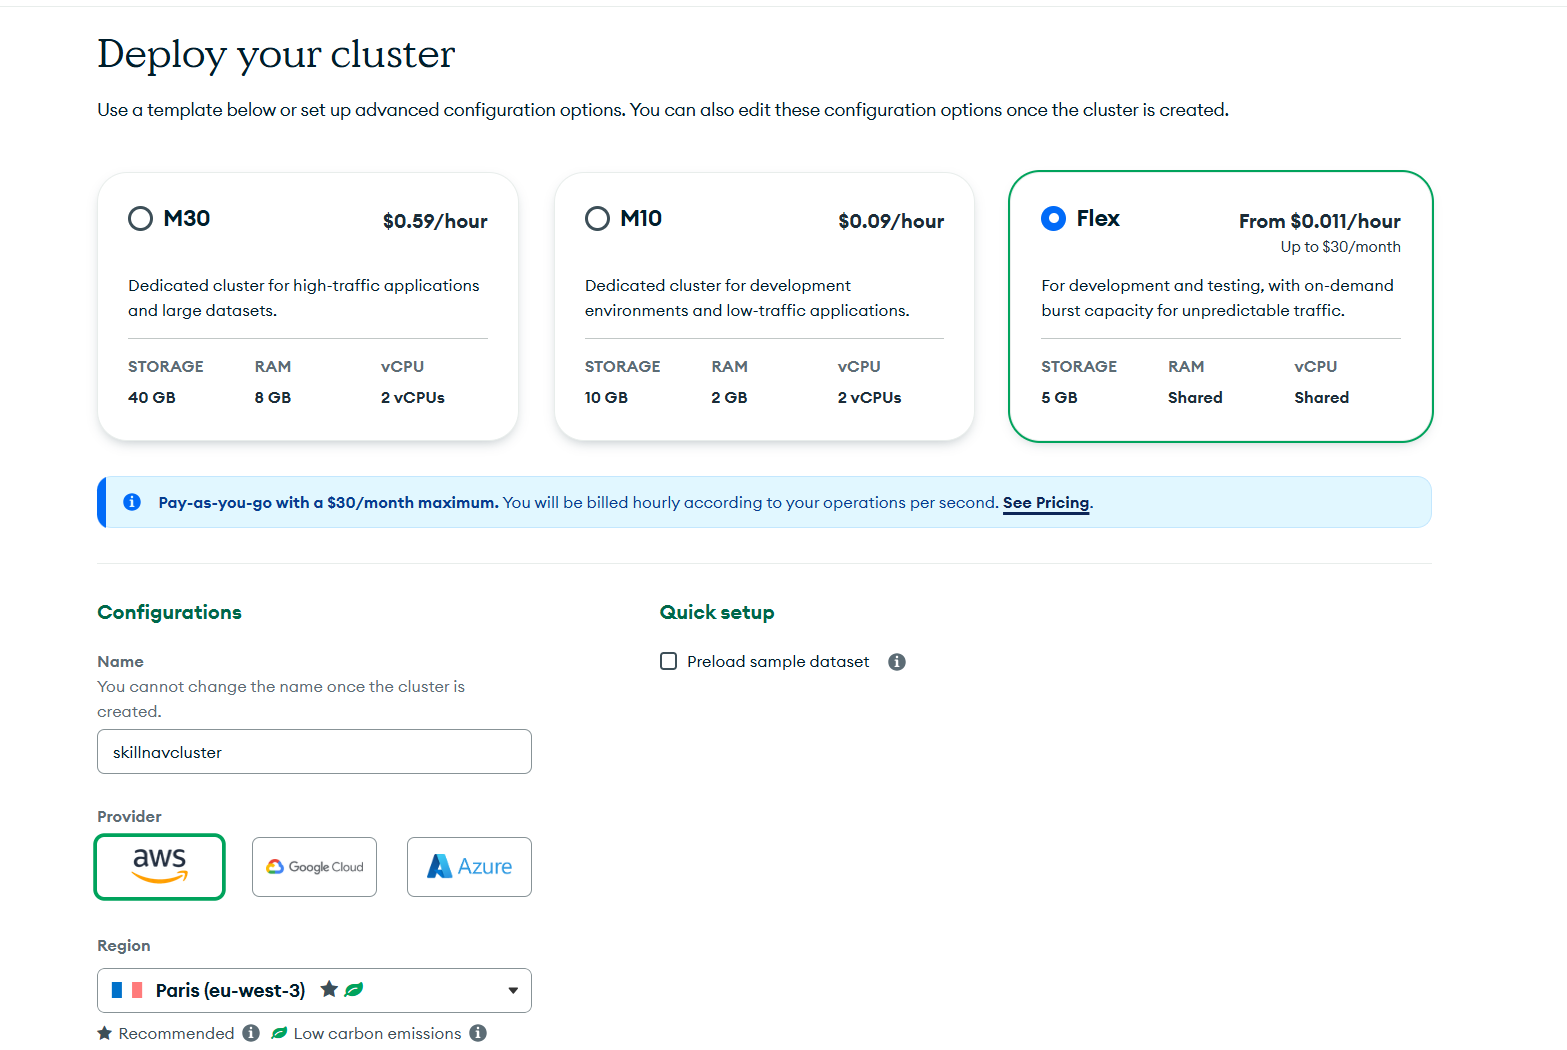
\includegraphics[width=\textwidth]{mongodb_cluster_creation.png}
    \caption{Cr\'eation du cluster Atlas en M0 Free Tier.}
  \end{subfigure}\hfill
  \begin{subfigure}[t]{0.48\textwidth}
    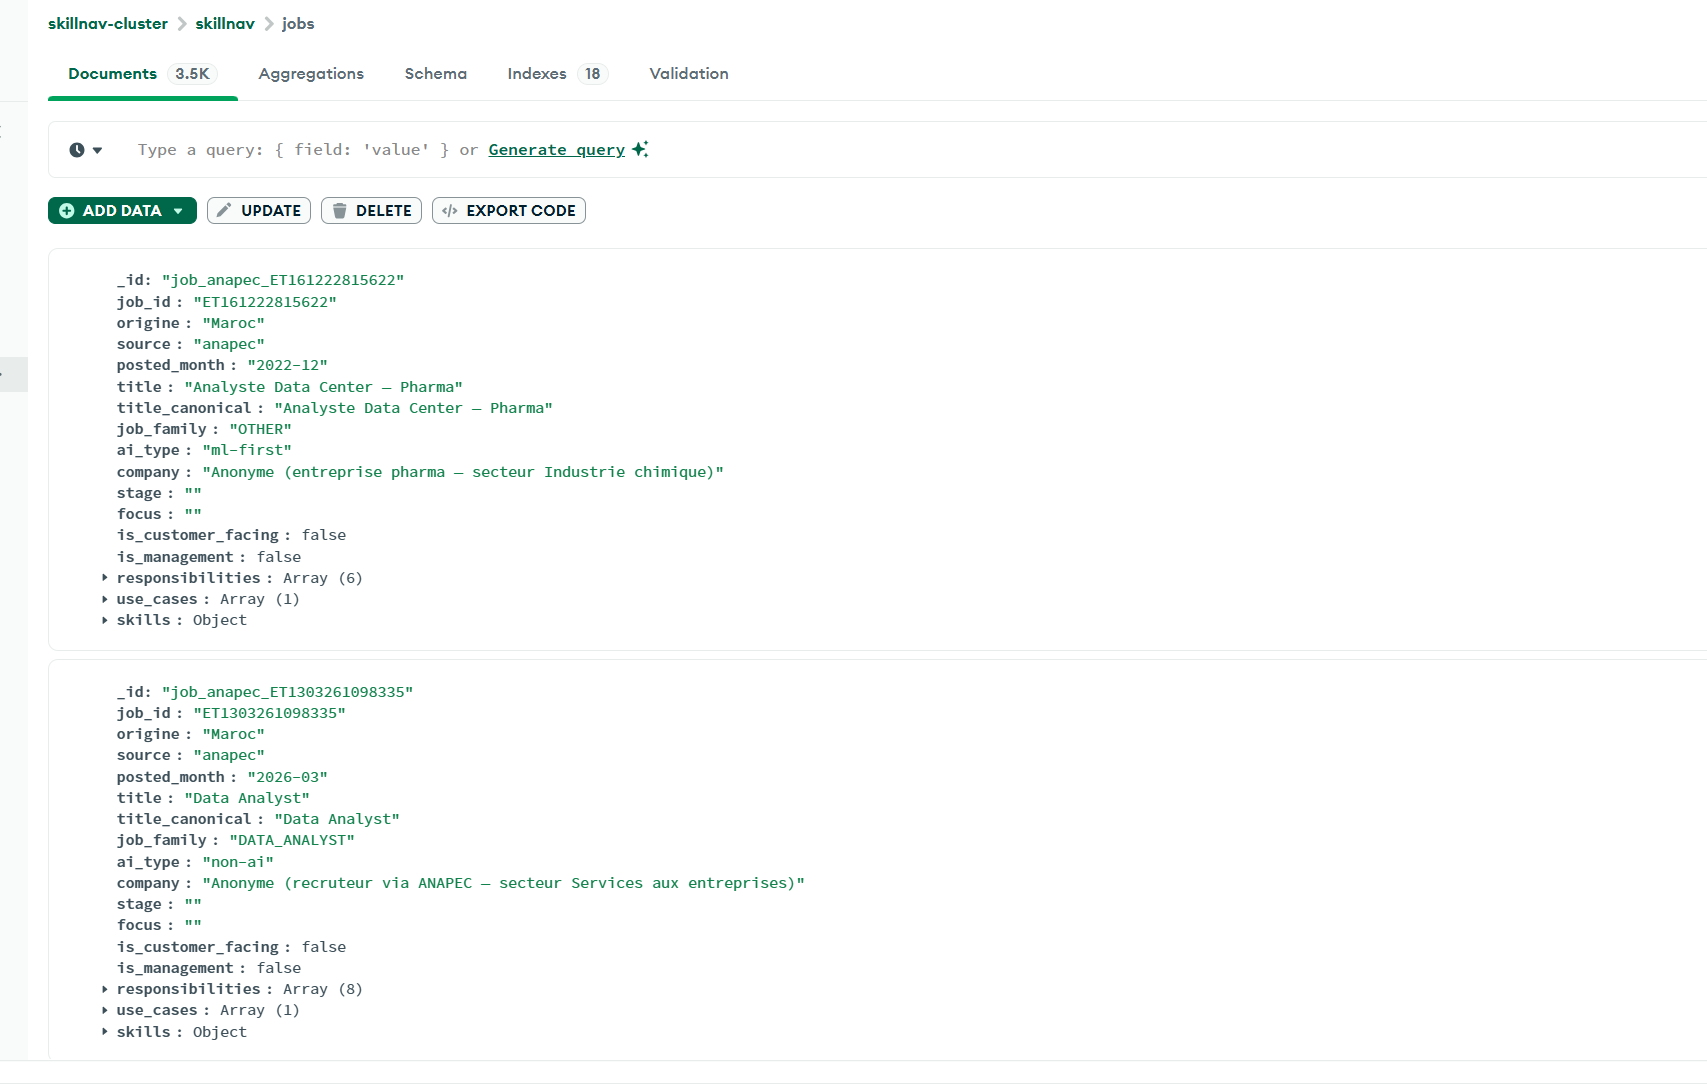
\includegraphics[width=\textwidth]{mongodb_ingestion.png}
    \caption{Ingestion des 3\,467 documents apr\`es 18 s d'upsert.}
  \end{subfigure}
  \caption{D\'eploiement et ingestion sur MongoDB Atlas.}
  \label{fig:mongodb-deploy}
\end{figure}

\subsection{Neo4j AuraDB pour le graphe de comp\'etences}

Le graphe de comp\'etences \skillnav est h\'eberg\'e sur une instance Neo4j AuraDB en formule Free Tier. Ce choix est motiv\'e par la richesse des requ\^etes natives offertes par le langage Cypher, par l'int\'egration directe de la biblioth\`eque Graph Data Science (GDS) qui impl\'emente nativement les algorithmes PageRank, Louvain et Leiden, et par l'h\'ebergement manag\'e sans installation locale.

Le sch\'ema du graphe comporte quatre types de n\oe uds et quatre types d'ar\^etes, dont la documentation d\'etaill\'ee figure dans l'annexe~A.

\begin{lstlisting}[language={},numbers=none,caption={Sch\'ema topologique du graphe Neo4j}]
       (Company)--[:POSTED_BY]-->(Job)
                                  |
                                  +--[:REQUIRES {confidence}]-->(Skill)
                                                                  |
                                                                  +--[:BELONGS_TO]-->(SkillFamily)
                                                                  |
                                                                  +--[:CO_OCCURS_WITH {weight}]--(Skill)
\end{lstlisting}

Les n\oe uds \texttt{Skill} (3\,937 instances) portent les propri\'et\'es \texttt{name}, \texttt{family} (parmi quatorze valeurs de l'\'enum\'eration \texttt{SkillFamily}), \texttt{pagerank\_score}, \texttt{community\_id} et \texttt{occurrence\_count}. Les n\oe uds \texttt{Job} (3\,467 instances) portent les propri\'et\'es \texttt{job\_id}, \texttt{title}, \texttt{company}, \texttt{country}, \texttt{source} et \texttt{published\_at}. Les n\oe uds \texttt{Company} (1\,515 instances) portent \texttt{name}, \texttt{country} et \texttt{job\_count}. Les n\oe uds \texttt{SkillFamily} (14 instances) portent \texttt{name} et \texttt{description}.

Les ar\^etes pond\'er\'ees \texttt{REQUIRES} (23\,170 instances) relient un Job \`a chacune de ses comp\'etences. Les ar\^etes non orient\'ees \texttt{CO\_OCCURS\_WITH} (10\,324 instances apr\`es filtrage \texttt{min\_cooccurrence=2}) relient deux comp\'etences co-occurrentes avec un poids \'egal au nombre d'offres dans lesquelles elles apparaissent ensemble. Les ar\^etes \texttt{BELONGS\_TO} (3\,937 instances) relient chaque comp\'etence \`a sa famille. Les ar\^etes \texttt{POSTED\_BY} (3\,467 instances) relient chaque entreprise aux offres qu'elle publie. La volum\'etrie totale s'\'el\`eve \`a 8\,934 n\oe uds et 40\,899 relations.

\subsection{OpenSearch via Bonsai pour la recherche full-text}

La recherche plein texte et les agr\'egations rapides du dashboard \skillnav sont assur\'ees par un cluster OpenSearch h\'eberg\'e chez Bonsai en formule Sandbox. Le choix de OpenSearch plut\^ot qu'Elasticsearch Enterprise repose sur deux crit\`eres. Le premier est la \textbf{p\'erennit\'e} : Elasticsearch Cloud en formule Free est limit\'e \`a quatorze jours d'essai, ce qui ferait expirer la d\'emonstration avant la soutenance du 28 mai 2026. Bonsai Sandbox est gratuit de mani\`ere permanente. Le second crit\`ere est la \textbf{licence} : OpenSearch est distribu\'e sous Apache 2.0 alors qu'Elasticsearch est sous double licence AGPL et Elastic License v2 ; la licence Apache 2.0 est plus simple \`a justifier juridiquement pour un projet acad\'emique.

Bonsai Sandbox provisionne une instance OpenSearch 2.19.5. L'index \texttt{skillnav\_jobs} est cr\'e\'e avec un analyzer personnalis\'e \texttt{fr\_en\_mixed} (combinaison du tokenizer standard et des filtres lowercase, asciifolding) qui couvre correctement le fran\c{c}ais et l'anglais sans dictionnaire externe. Les champs principaux sont mapp\'es avec deux types distincts : champs \texttt{text} analys\'es pour la recherche full-text avec scoring BM25 (titre, responsabilit\'es, cas d'usage), et champs \texttt{keyword} non analys\'es pour les filtres exacts et les agr\'egations.

L'ingestion des 3\,467 fiches s'effectue depuis le m\^eme fichier consolid\'e \texttt{data/jobs.jsonl} via le script \texttt{scripts/ingestion/ingest\_elasticsearch.py}, en environ quatre secondes et demie (vitesse moyenne de 772 documents par seconde, sup\'erieure \`a MongoDB gr\^ace \`a la nature optimis\'ee de l'API \texttt{\_bulk}).

\subsection{Pipeline de transmission YAML vers JSON Lines vers bases cibles}

Le passage des donn\'ees depuis le format de stockage humain (YAML) vers les trois bases cibles s'effectue par l'interm\'ediaire d'un format de transmission unifi\'e, le \textbf{JSON Lines}, dans lequel chaque ligne contient un objet JSON ind\'ependant. Ce format combine les avantages du JSON (interop\'erabilit\'e universelle) avec ceux du traitement par flux (lecture ligne par ligne sans charger la totalit\'e du fichier en m\'emoire). Il est consomm\'e nativement par les utilitaires d'ingestion bulk des trois bases retenues : \texttt{mongoimport --type jsonl} pour MongoDB Atlas, API \texttt{\_bulk} pour OpenSearch, et requ\^etes Cypher \texttt{UNWIND} pour Neo4j.

Le script de transformation \texttt{scripts/build\_dataset.py} enchaine trois \'etapes pour produire le fichier \texttt{data/jobs.jsonl} : parcours r\'ecursif des YAML via \texttt{Path.rglob('*.yaml')} et chargement en m\'emoire ; canonicalisation \`a trois niveaux d\'etaill\'ee en section~2.3.4 ; s\'erialisation en JSON Lines et g\'en\'eration de deux fichiers CSV (\texttt{graph\_nodes.csv} et \texttt{graph\_edges.csv}) consommables alternativement par Neo4j via \texttt{LOAD CSV}. L'ensemble s'ex\'ecute en environ une minute et est rigoureusement idempotent.

\section{Pipeline Content Mining}

\subsection{Nettoyage et d\'etection de langue}

Le pipeline Content Mining traite s\'equentiellement chaque offre extraite par les scrapers selon quatre \'etapes successives. La premi\`ere \'etape de nettoyage consiste \`a convertir le HTML brut en Markdown propre exploitable par les mod\`eles d'extraction structur\'ee. La biblioth\`eque Crawl4AI est utilis\'ee \`a cette fin et produit un rendu qui pr\'eserve la structure hi\'erarchique des titres et des listes tout en \'eliminant les balises HTML accessoires. La d\'etection automatique de la langue principale est effectu\'ee par la biblioth\`eque \texttt{fasttext-langdetect} avec une pr\'ecision sup\'erieure \`a 98\,\% sur des textes techniques de plus de cent caract\`eres. La tokenisation pr\'eparatoire est confi\'ee \`a spaCy avec le mod\`ele \texttt{fr\_core\_news\_md} pour les documents francophones, \texttt{en\_core\_web\_md} pour les anglophones, avec fallback automatique sur \texttt{xx\_ent\_wiki\_sm}.

\subsection{Extraction structur\'ee par Pydantic AI et Claude Sonnet 4.5}

L'extraction structur\'ee constitue l'\'etape centrale du pipeline Content Mining. Elle est confi\'ee au mod\`ele Claude Sonnet 4.5 d'Anthropic, mobilis\'e via la biblioth\`eque Pydantic AI qui fournit une couche d'abstraction entre le prompt et la sortie typ\'ee. Le sch\'ema Pydantic v2 cible est d\'efini dans le module \texttt{skillnav/schemas/job.py} et formalise la sortie attendue selon la classe \texttt{JobExtraction}, qui comporte une trentaine de champs typ\'es couvrant l'intitul\'e de poste, l'entreprise, la localisation, le pays, le type de contrat, le niveau de s\'eniorit\'e, les listes de comp\'etences, la source, l'URL d'origine, la date de publication, la langue d\'etect\'ee et un score de confiance global.

L'architecture Pydantic AI assure la validation automatique de la sortie : tout document dont l'extraction ne satisfait pas le sch\'ema d\'eclar\'e est rejet\'e avec une erreur explicite, ce qui \'elimine les hallucinations classiques de format. Une strat\'egie de \textbf{seuil de confiance} est appliqu\'ee : tout document dont le score retourn\'e par Claude est strictement inf\'erieur \`a 0,75 est marqu\'e avec le statut \texttt{JobStatus.QUARANTINED} et exclu des analyses statistiques en aval. Le statut \texttt{JobStatus.EXTRACTED} est attribu\'e aux documents valid\'es.

\subsection{Reconnaissance d'entit\'es nomm\'ees}

L'\'etape de reconnaissance d'entit\'es nomm\'ees est conduite de mani\`ere comparative entre trois mod\`eles transformer issus de la biblioth\`eque Hugging Face : BERT multilingue (\texttt{Davlan/bert-base-multilingual-cased-ner-hrl}), CamemBERT-NER (\texttt{Jean-Baptiste/camembert-ner}) et DistilBERT-NER (\texttt{dslim/distilbert-NER}). Ces trois mod\`eles sont charg\'es via le pipeline NER de la biblioth\`eque \texttt{transformers} et appliqu\'es \`a chaque offre du gold set de trente fiches, dont la composition et les r\'esultats d\'etaill\'es sont report\'es en section~4.2.

\subsection{Normalisation taxonomique}

La quatri\`eme \'etape consiste \`a canonicaliser le vocabulaire extrait pour r\'eduire les variations orthographiques et typographiques. Trois niveaux de canonicalisation sont appliqu\'es s\'equentiellement, document\'es dans le module \texttt{scripts/skillnav\_eda.py}.

Le premier niveau concerne les comp\'etences : un dictionnaire \texttt{SKILL\_ALIASES} contenant plus de 190 alias mappe les variantes les plus fr\'equentes vers leur forme canonique (par exemple \texttt{LLM}, \texttt{LLMs}, \texttt{llm}, \texttt{Large Language Model} sont tous canonicalis\'es en \texttt{LLM}).

Le deuxi\`eme niveau concerne les intitul\'es de poste : la fonction \texttt{strip\_gender\_suffix} retire les suffixes de parit\'e (\texttt{H/F}, \texttt{F/H}, \texttt{M/F}, \texttt{(m/f/x)}), le dictionnaire \texttt{TITLE\_ALIASES} mappe les trente intitul\'es les plus fr\'equents, et la fonction \texttt{smart\_title\_case} applique une mise en Title Case qui pr\'eserve les acronymes connus (AI, ML, NLP, MLOps, LLM, RAG, etc.).

Le troisi\`eme niveau concerne la famille de poste : la fonction \texttt{detecter\_famille\_poste} mappe l'intitul\'e brut vers l'une des treize familles via des expressions r\'eguli\`eres ordonn\'ees du plus sp\'ecifique au plus g\'en\'eral.

L'effet combin\'e des trois niveaux de canonicalisation est mesurable empiriquement : le vocabulaire des comp\'etences extraites brutes comportait 11\,000 entr\'ees distinctes avant canonicalisation, et 8\,082 entr\'ees canoniques apr\`es, soit une r\'eduction de 27\,\% du vocabulaire.

\section{Pipeline Structure Mining}

\subsection{Construction du graphe Skill vers Skill par co-occurrence}

La mod\'elisation du march\'e des comp\'etences sous forme de graphe est construite par projection de \textbf{co-occurrence} entre paires de comp\'etences dans la m\^eme offre d'emploi. L'algorithme, impl\'ement\'e dans le module \texttt{skillnav/pipelines/structure\_mining/graph\_builder.py}, parcourt les 3\,467 offres du corpus consolid\'e, extrait pour chaque offre l'ensemble d\'edoublonn\'e de ses comp\'etences, g\'en\`ere toutes les paires non ordonn\'ees via \texttt{itertools.combinations}, et incr\'emente un compteur de co-occurrences pour chaque paire. Le graphe final comporte 3\,937 n\oe uds Skill et 10\,324 ar\^etes pond\'er\'ees apr\`es application du seuil minimum de co-occurrence justifi\'e en section~2.4.3.

\subsection{Justification de la projection plut\^ot que d'un graphe bipartite}

La mod\'elisation alternative qui consisterait \`a conserver les Jobs comme n\oe uds interm\'ediaires dans un graphe bipartite Job vers Skill n'est pas retenue, pour des raisons document\'ees dans la litt\'erature du skill mining. Cetin et al. (2023) montrent que les algorithmes de d\'etection de communaut\'es appliqu\'es \`a un graphe bipartite produisent des communaut\'es mixtes qui m\'elangent Jobs et Skills, et dont l'interpr\'etation s\'emantique est faible. Decorte et al. (2022) confirment cette observation sur un corpus de 100\,000 offres internationales et recommandent la projection Skill vers Skill par co-occurrence pond\'er\'ee comme mod\'elisation canonique.

La projection Skill vers Skill pr\'esente trois avantages : elle \'elimine les Jobs comme n\oe uds interm\'ediaires dans la composante trait\'ee par les algorithmes de communaut\'es, produisant des communaut\'es pures de comp\'etences ; elle pond\`ere naturellement chaque ar\^ete par le nombre d'offres dans lesquelles deux comp\'etences co-occurrent ; elle correspond \`a la mod\'elisation standard de la litt\'erature, garantissant la comparabilit\'e des r\'esultats. Les n\oe uds Job, Company et SkillFamily restent toutefois pr\'esents dans Neo4j AuraDB pour permettre les requ\^etes crois\'ees expos\'ees par le dashboard.

\subsection{Filtrage du bruit par seuil de co-occurrence}

L'application brute de la projection Skill vers Skill sans filtrage produirait un graphe noy\'e sous le bruit des co-occurrences fortuites. Une offre exotique mentionnant simultan\'ement trente comp\'etences h\'et\'erog\`enes g\'en\'ererait \`a elle seule 435 ar\^etes, dont la grande majorit\'e n'aurait aucune signification statistique. Pour r\'eduire ce bruit, un seuil minimum de co-occurrence est appliqu\'e par le param\`etre \texttt{min\_cooccurrence=2}. Concr\`etement, une paire de comp\'etences n'est conserv\'ee comme ar\^ete du graphe que si elle appara\^it dans au moins deux offres distinctes du corpus. Sans ce filtre, le graphe comporterait approximativement 75\,000 ar\^etes au lieu de 10\,324, dont environ 65\,000 ar\^etes fortuites de poids unitaire.

\subsection{Centralit\'e par PageRank}

L'algorithme PageRank (Page et al., 1999), originellement d\'evelopp\'e pour le classement des pages web par Google, est appliqu\'e au graphe Skill vers Skill pour identifier les comp\'etences les plus structurantes du march\'e. Impl\'ement\'e dans \texttt{skillnav/pipelines/structure\_mining/pagerank.py}, il est ex\'ecut\'e avec un facteur d'amortissement \texttt{alpha=0.85} (valeur standard de la litt\'erature) et un poids d'ar\^ete \'egal au nombre de co-occurrences. Le r\'esultat est un score \texttt{pagerank\_score} attribu\'e \`a chaque n\oe ud Skill, dont les valeurs les plus \'elev\'ees identifient les \textbf{comp\'etences pivot} du march\'e. Le d\'etail des r\'esultats et le classement top 20 sont report\'es en section~4.3.4.

\subsection{D\'etection de communaut\'es}

Trois algorithmes de d\'etection de communaut\'es sont impl\'ement\'es et compar\'es dans \texttt{skillnav/pipelines/structure\_mining/communities.py}. Louvain (Blondel et al., 2008) est impl\'ement\'e via \texttt{python-louvain} et applique une strat\'egie it\'erative gloutonne maximisant la modularit\'e de Newman (2006). Leiden (Traag et al., 2019) est impl\'ement\'e via \texttt{igraph} et constitue une am\'elioration de Louvain garantissant la connexit\'e interne des communaut\'es d\'etect\'ees. Label Propagation (Raghavan et al., 2007) est impl\'ement\'e via \texttt{networkx} et constitue un algorithme baseline rapide mais non d\'eterministe. Le d\'etail du protocole exp\'erimental et les r\'esultats chiffr\'es sont report\'es en section~4.3.

\section{Pipeline Usage Mining}

\subsection{Construction des s\'eries temporelles hebdomadaires}

Le pipeline Usage Mining transforme les fiches dat\'ees en s\'eries temporelles exploitables par les mod\`eles de forecasting. L'algorithme, impl\'ement\'e dans \texttt{skillnav/pipelines/usage\_mining/series\_builder.py}, op\`ere en cinq \'etapes : filtrage des fiches dont la date \texttt{posted\_date} est exploitable et post\'erieure au 1\textsuperscript{er} janvier 2026 ; calcul pour chaque fiche de la semaine ISO de publication ; identification des \texttt{top\_n} comp\'etences les plus fr\'equentes globalement ; comptage des occurrences hebdomadaires ; production d'une liste \texttt{SkillTimeSeries} Pydantic avec remplissage par z\'ero pour les semaines sans occurrence.

\subsection{Justification de la fen\^etre temporelle}

La fen\^etre temporelle retenue pour le forecasting s'\'etend du 1\textsuperscript{er} janvier 2026 \`a fin avril 2026, soit environ vingt-deux semaines ISO compl\`etes. Ce choix est dict\'e par deux consid\'erations. Premi\`erement, la \textbf{densit\'e de couverture} du corpus n'est suffisante qu'\`a partir de janvier 2026 (volume hebdomadaire d\'epassant durablement la centaine). Avant cette date, les semaines comportent typiquement moins de vingt fiches et produisent des s\'eries trop bruit\'ees. Deuxi\`emement, un \textbf{artefact de collecte} affecte les trois derni\`eres semaines de la fen\^etre (27 avril au 17 mai 2026) : la collecte du corpus ayant \'et\'e effectu\'ee autour du 14-16 mai 2026, les fiches publi\'ees tardivement n'avaient pas encore \'et\'e index\'ees. Le param\`etre \texttt{truncate\_last\_weeks=3} retire automatiquement ces trois semaines, ce qui laisse une s\'erie effective de seize semaines.

\subsection{Partition train, test et horizon}

Le partitionnement retenu affecte les seize semaines exploitables en quinze semaines d'entra\^inement et quatre semaines de test, avec un horizon suppl\'ementaire de quatre semaines de pr\'ediction future. Param\'etr\'e dans \texttt{skillnav/pipelines/usage\_mining/comparison.py} par les variables \texttt{train\_periods=15}, \texttt{test\_periods=4} et \texttt{horizon=4}, ce partitionnement r\'eserve une portion de test substantielle (de l'ordre de 20\,\% de la s\'erie) tout en conservant assez d'historique pour l'estimation des param\`etres autor\'egressifs.

\subsection{Forecasting comparatif ARIMA, Prophet et LSTM}

Trois mod\`eles de forecasting issus de familles algorithmiques distinctes sont impl\'ement\'es et compar\'es. Le mod\`ele ARIMA (AutoRegressive Integrated Moving Average), dans la formulation classique de Box et Jenkins (1976), est impl\'ement\'e via \texttt{statsmodels} avec s\'election automatique des param\`etres \texttt{(p, d, q)} par minimisation du crit\`ere d'information d'Akaike. Le mod\`ele Prophet, d\'evelopp\'e par Taylor et Letham (2018) chez Meta, est impl\'ement\'e via la biblioth\`eque \'eponyme \texttt{prophet}, dont la d\'ecomposition additive en tendance, saisonnalit\'e et termes r\'esiduels convient aux s\'eries pr\'esentant une saisonnalit\'e forte. Le mod\`ele LSTM (Hochreiter et Schmidhuber, 1997), r\'eseau neuronal r\'ecurrent, est impl\'ement\'e via \texttt{neuralforecast} de Nixtla, avec une architecture compacte adapt\'ee \`a la longueur courte des s\'eries.

\subsection{M\'etriques d'\'evaluation et choix de la m\'etrique de s\'election}

Quatre m\'etriques d'\'evaluation sont calcul\'ees syst\'ematiquement pour chaque mod\`ele et chaque comp\'etence. Le \textbf{MAPE robuste} est calcul\'e uniquement sur les semaines o\`u la valeur r\'eelle observ\'ee est sup\'erieure ou \'egale \`a cinq, ce qui \'evite la division par des valeurs nulles. Le \textbf{RMSE} calcule la racine carr\'ee de la moyenne des carr\'es des erreurs et p\'enalise fortement les grosses erreurs ponctuelles. Le \textbf{MAE} fournit une mesure plus robuste aux valeurs aberrantes que RMSE. Le \textbf{taux de couverture de l'intervalle de confiance \`a 95\,\%} mesure le pourcentage de valeurs r\'eelles \`a l'int\'erieur de l'intervalle retourn\'e par le mod\`ele.

La m\'etrique principale retenue pour la \textbf{s\'election du meilleur mod\`ele} est le RMSE. Trois raisons motivent ce choix : RMSE est robuste aux s\'eries comportant des semaines \`a z\'ero occurrence (contrairement au MAPE qui explose) ; RMSE poss\`ede la m\^eme unit\'e que la variable observ\'ee, ce qui le rend directement interpr\'etable ; la p\'enalisation des grosses erreurs convient au cas d'usage \skillnav.

\section{Data Quality Framework}

\subsection{Compl\'etude des champs}

L'\'evaluation de la compl\'etude du corpus est conduite en mesurant le taux de remplissage de chaque champ du sch\'ema Pydantic \texttt{JobExtraction} sur les 3\,467 fiches consolid\'ees. Les champs obligatoires (\texttt{title}, \texttt{company}, \texttt{source}, \texttt{source\_url}, \texttt{scraped\_at}) pr\'esentent par construction un taux de compl\'etude de 100\,\%, garanti par la validation Pydantic. Les champs facultatifs pr\'esentent des taux variables : 100\,\% sur \texttt{description} (apr\`es l'op\'eration de recovery), 98\,\% sur \texttt{country}, 92\,\% sur \texttt{posted\_date}, 87\,\% sur \texttt{contract\_type}, et 65\,\% sur \texttt{seniority}.

\subsection{D\'etection du bruit}

La d\'etection des fiches bruit\'ees ou redondantes est conduite selon trois crit\`eres automatis\'es. Le premier crit\`ere est la \textbf{d\'etection de doublons par empreinte SHA-256} calcul\'ee sur la concat\'enation des champs \texttt{company}, \texttt{title} et \texttt{source\_url}. Sur le corpus \skillnav, aucun doublon strict n'a \'et\'e d\'etect\'e apr\`es application de la canonicalisation, ce qui valide la qualit\'e des identifiants sources. Le deuxi\`eme crit\`ere identifie les \textbf{titres anormalement courts} (moins de cinq caract\`eres apr\`es normalisation). Le troisi\`eme crit\`ere identifie les \textbf{descriptions anormalement courtes} (moins de 200 caract\`eres), qui correspondent typiquement \`a des annonces tronqu\'ees ou expir\'ees. Dix-sept fiches incompl\`etes ont \'et\'e \'elimin\'ees du corpus consolid\'e en mai 2026.

\subsection{Biais reconnus}

Cinq biais structurels sont reconnus et document\'es explicitement dans le projet plut\^ot que masqu\'es par une correction artificielle. Le \textbf{biais linguistique} r\'esulte de la composition mixte du corpus (73\,\% des fiches en anglais, 27\,\% en fran\c{c}ais) et affecte directement la performance des mod\`eles NER. Le \textbf{biais g\'eographique} r\'esulte de l'asym\'etrie de volum\'etrie (381 fiches Maroc contre 3\,086 fiches International). Le \textbf{biais de plateforme} refl\`ete les pratiques \'editoriales diff\'erenci\'ees des sources (LinkedIn favorise les descriptions longues, Rekrute privil\'egie les annonces synth\'etiques, Glassdoor reproduit verbatim). Le \textbf{biais sectoriel} r\'esulte de la sur-repr\'esentation de certains secteurs (services financiers sur \texttt{builtin.com}, conseil au Maroc). Le \textbf{biais lexical de genre} refl\`ete les usages encore majoritairement masculins des intitul\'es en fran\c{c}ais, neutralis\'es par \texttt{strip\_gender\_suffix} sur les suffixes connus.

La \textbf{strat\'egie de transparence} retenue par le projet consiste \`a visualiser explicitement ces biais sur le dashboard \skillnav (page \texttt{/quality}) plut\^ot que de les corriger par re-pond\'eration. Ce choix est d\'efendable scientifiquement : la correction artificielle masquerait la r\'ealit\'e du march\'e observ\'e.

\subsection{M\'ethodologie d'\'evaluation}

L'\'evaluation syst\'ematique du framework de Data Quality est impl\'ement\'ee dans le notebook \texttt{01\_data\_quality.ipynb}, dont la finalisation est planifi\'ee en parall\`ele de la r\'edaction du pr\'esent rapport. Le notebook produit cinq tableaux de synth\`ese : compl\'etude par champ et par source, distribution des longueurs de descriptions par source, taux de doublons par crit\`ere, distribution des langues par source, et tableau r\'ecapitulatif des biais reconnus.

% =============== CHAPITRE 3 =================================
\chapter{Analyse exploratoire du corpus}

Le pr\'esent chapitre fournit une lecture chiffr\'ee et visuelle du corpus \skillnav constitu\'e de 3\,467 fiches d'offres d'emploi consolid\'ees au 16 mai 2026. L'analyse est volontairement descriptive : son objectif est de d\'egager les tendances structurelles du march\'e des comp\'etences en Intelligence Artificielle et Data Science, sans encore introduire les \'etudes comparatives algorithmiques qui font l'objet du chapitre~4. Les seize figures pr\'esent\'ees ci-apr\`es sont produites par le notebook \texttt{01\_visualisations.ipynb} \`a partir du fichier consolid\'e \texttt{data/jobs.jsonl}.

L'analyse exploratoire est organis\'ee en trois temps. Une lecture macroscopique caract\'erise d'abord la volum\'etrie et la composition du corpus. Une lecture par sous-corpus examine ensuite s\'epar\'ement le march\'e marocain puis le march\'e international. Une lecture comparative met enfin en \'evidence les \'ecarts les plus significatifs entre les deux march\'es.

\section{Bascule structurelle du march\'e apr\`es la sortie de ChatGPT}

La sortie publique de ChatGPT en novembre 2022 constitue le point d'ancrage de l'observation. Cet \'ev\'enement est consid\'er\'e dans la litt\'erature comme un choc structurel sur le march\'e des comp\'etences en Intelligence Artificielle, dans la mesure o\`u il a popularis\'e l'usage des mod\`eles de langage de grande taille aupr\`es du grand public et d\'eclench\'e une vague d'adoption sans pr\'ec\'edent dans les directions d'entreprise (World Economic Forum, 2025). Le corpus \skillnav couvre une fen\^etre temporelle s'\'etendant d'ao\^ut 2022 \`a mai 2026, ce qui permet d'observer empiriquement l'\'evolution du march\'e autour de ce point de bascule.

\begin{figure}[H]
  \centering
  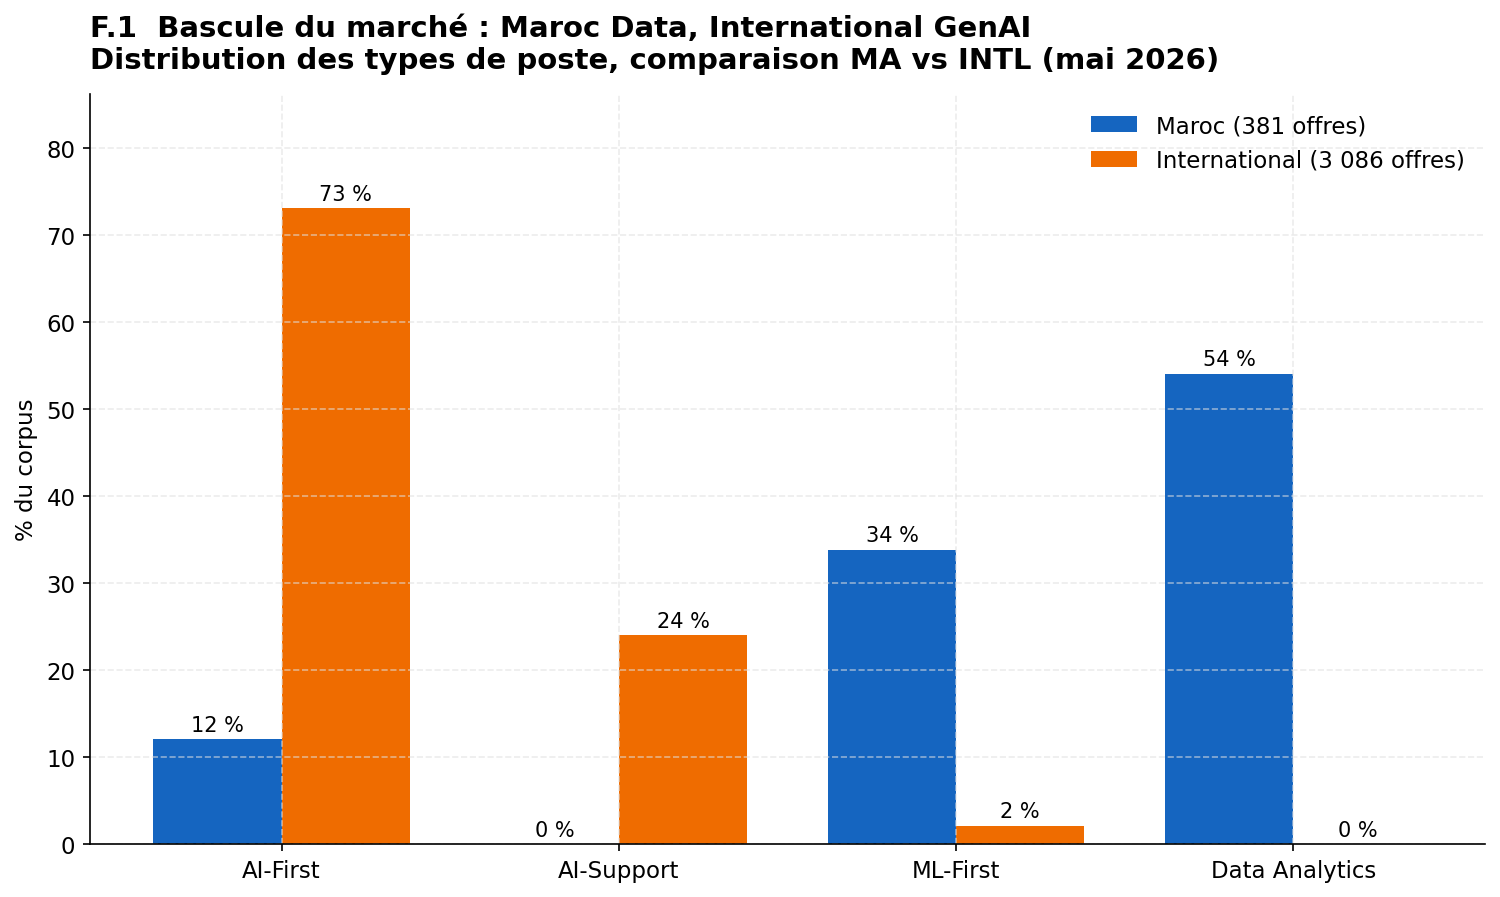
\includegraphics[width=0.85\textwidth]{f01_bascule_marche.png}
  \caption{Bascule structurelle du march\'e des comp\'etences IA apr\`es la sortie de ChatGPT en novembre 2022.}
  \label{fig:f01-bascule}
\end{figure}

La figure~\ref{fig:f01-bascule} met en \'evidence un saut quantitatif observable d\`es le premier trimestre 2023 sur les comp\'etences typiques de l'Intelligence Artificielle g\'en\'erative, en particulier les mod\`eles de langage, les architectures de g\'en\'eration augment\'ee par r\'ecup\'eration (Retrieval-Augmented Generation, ou RAG) et l'ing\'enierie de prompts. Ce constat empirique valide l'hypoth\`ese retenue par le projet, \`a savoir que la p\'eriode 2023 \`a 2026 constitue une fen\^etre d'observation pertinente pour mesurer la diffusion des comp\'etences en Intelligence Artificielle g\'en\'erative dans les annonces d'emploi.

\section{Volumes et distribution}

\subsection{Distribution par origine et par source}

Le corpus consolid\'e regroupe 3\,467 fiches d'offres apr\`es canonicalisation et d\'eduplication. Il se d\'ecompose en 381 fiches collect\'ees au Maroc et 3\,086 fiches collect\'ees \`a l'international. La distribution par source est pr\'esent\'ee dans le tableau~\ref{tab:distribution-sources}.

\begin{table}[H]
  \centering
  \caption{Distribution des 3\,467 fiches consolid\'ees par origine et par source.}
  \label{tab:distribution-sources}
  \small
  \begin{tabularx}{\textwidth}{l L{4.5cm} r L{2.8cm} L{3.2cm}}
    \toprule
    \rowcolor{softblue}\textbf{Origine} & \textbf{Source} & \textbf{Postings} & \textbf{P\'eriode} & \textbf{M\'ethode} \\
    \midrule
    Maroc & ANAPEC & 2 & 2026-05 & Playwright \\
    Maroc & Rekrute & 27 & 2023-2026 & Playwright \\
    Maroc & Indeed MA & 67 & 2025-2026 & Apify + recovery \\
    Maroc & LinkedIn MA & 207 & 2025-2026 & Apify \\
    Maroc & Pages carri\`eres MA & 6 & 2026-05 & Firecrawl + JSON-LD \\
    Maroc & Glassdoor MA & 72 & 2025-2026 & Firecrawl + recovery \\
    INTL & Corpus Tech INTL (builtin.com) & 3\,086 & 2025-08 \`a 2026-04 & Pipeline 5 \'etapes \\
    \midrule
    \rowcolor{softblue}\textbf{Total} & & \textbf{3\,467} & \textbf{2022-08 \`a 2026-05} & \\
    \bottomrule
  \end{tabularx}
\end{table}

Le march\'e marocain est repr\'esent\'e par six sources distinctes couvrant une fen\^etre \'etendue et 147 entreprises distinctes. Le march\'e international est repr\'esent\'e par une source unique (le corpus Tech INTL import\'e depuis \texttt{builtin.com} selon le protocole d\'ecrit en section~2.1), couvrant six mois sur 1\,378 entreprises distinctes r\'eparties sur six pays (\'Etats-Unis, Inde, Royaume-Uni, Allemagne, Pays-Bas, et International g\'en\'erique). Cette asym\'etrie de volum\'etrie entre les deux sous-corpus est comment\'ee et discut\'ee comme limite de l'\'etude en section~5.2.1.

\subsection{Profils de poste accessoires}

Au-del\`a des intitul\'es principaux, le corpus pr\'esente deux indicateurs accessoires utiles \`a la caract\'erisation des march\'es. Au Maroc, 22 fiches (5,8\,\%) correspondent \`a des postes manag\'eriaux et 81 fiches (21,3\,\%) \`a des postes \`a interface client. \`A l'international, ces proportions s'\'el\`event respectivement \`a 14,9\,\% (459 fiches) et 22,4\,\% (692 fiches). L'\'ecart de repr\'esentation des postes manag\'eriaux entre les deux march\'es traduit la maturit\'e organisationnelle plus \'elev\'ee des structures internationales, qui disposent d'\'equipes d'Intelligence Artificielle suffisamment dimensionn\'ees pour justifier des fonctions d'encadrement sp\'ecialis\'ees.

\section{Distribution par type de poste : Maroc et International}

La classification automatique en quatre cat\'egories de postes (AI-First, AI-Support, ML-First, Data Analytics), r\'ealis\'ee au moment de la collecte par le mod\`ele Claude Sonnet 4.5 \`a partir du titre, des responsabilit\'es et des comp\'etences requises, r\'ev\`ele un contraste majeur entre les deux march\'es.

\begin{table}[H]
  \centering
  \caption{Distribution des types de poste dans les corpus Maroc et International.}
  \label{tab:types-postes}
  \begin{tabular}{lrrr}
    \toprule
    \rowcolor{softblue}\textbf{Type de poste} & \textbf{Maroc} & \textbf{International} & \textbf{\'Ecart (INTL - MA)} \\
    \midrule
    AI-First & 12,1\,\% & 73,1\,\% & +61,0 pts \\
    AI-Support & 0,0\,\% & 24,0\,\% & +24,0 pts \\
    ML-First & 33,9\,\% & 2,1\,\% & $-$31,8 pts \\
    Data Analytics & 54,1\,\% & 0,0\,\% & $-$54,1 pts \\
    Inconnu & 0,0\,\% & 0,7\,\% & +0,7 pt \\
    \bottomrule
  \end{tabular}
\end{table}

Ce tableau livre l'un des r\'esultats les plus structurants du projet. Le march\'e international, observ\'e depuis \texttt{builtin.com} sur les six derniers mois, est massivement orient\'e vers des profils AI-First (73,1\,\%), c'est-\`a-dire vers des postes o\`u l'Intelligence Artificielle g\'en\'erative constitue le produit lui-m\^eme. Le march\'e marocain, \`a l'inverse, reste domin\'e par des profils Data Analytics (54,1\,\%) et Machine Learning traditionnel (33,9\,\%), avec une pr\'esence tr\`es limit\'ee de profils AI-First (12,1\,\%) et une absence totale de profils AI-Support. Ce constat empirique fonde la pertinence du volet de gap analysis pr\'esent\'e au chapitre~5.1, lequel mesure dans quelle mesure les fili\`eres des \'Ecoles Nationales des Sciences Appliqu\'ees du Maroc pr\'eparent \`a un march\'e national dont la composition diff\`ere sensiblement du march\'e international de r\'ef\'erence.

\begin{figure}[H]
  \centering
  \begin{subfigure}[t]{0.48\textwidth}
    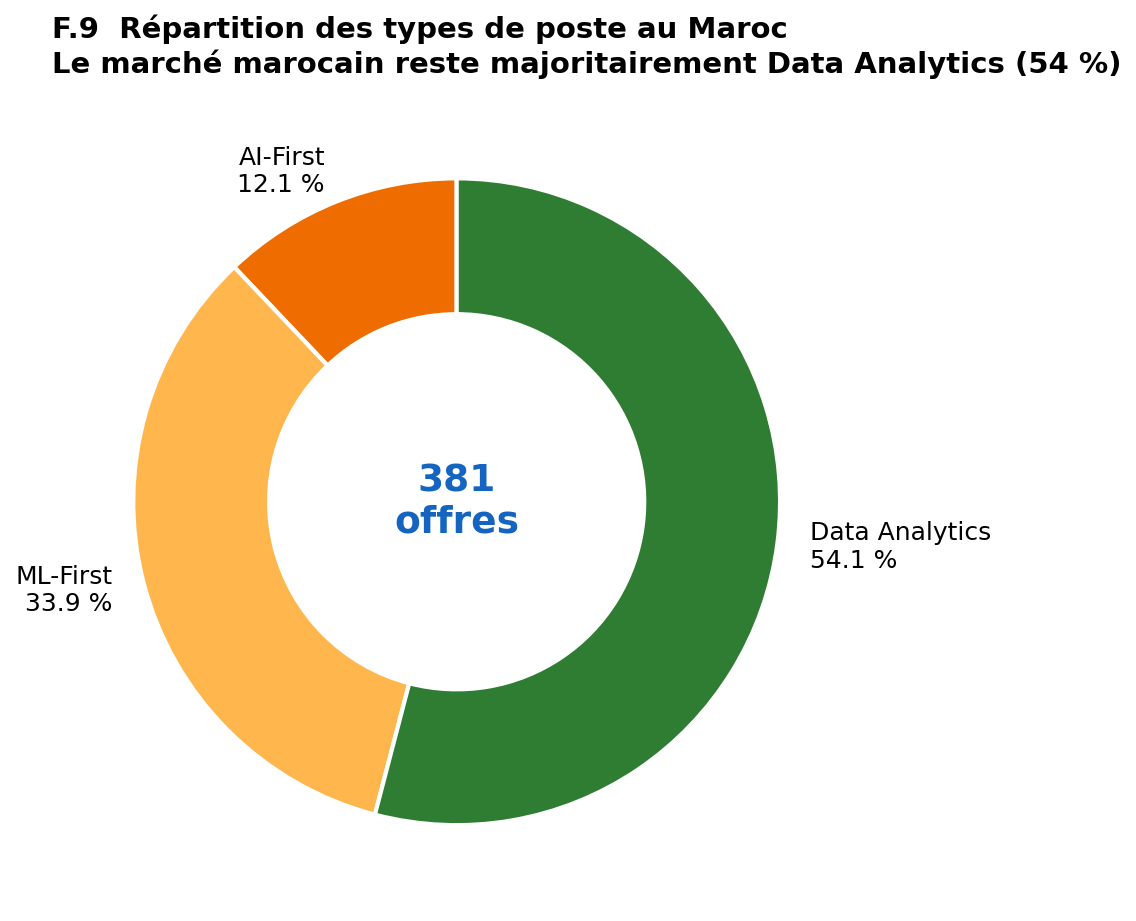
\includegraphics[width=\textwidth]{f09_distribution_types_maroc.png}
    \caption{Maroc (381 fiches).}
  \end{subfigure}\hfill
  \begin{subfigure}[t]{0.48\textwidth}
    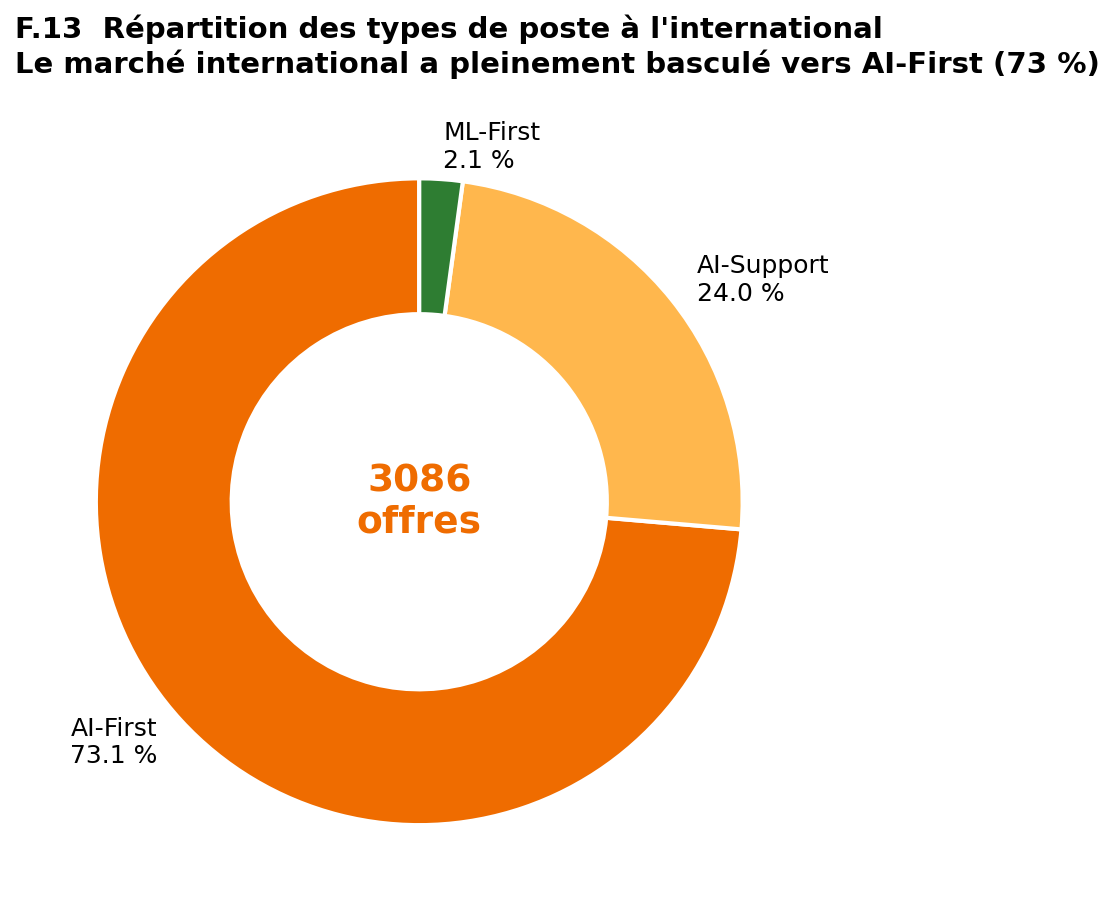
\includegraphics[width=\textwidth]{f13_distribution_types_intl.png}
    \caption{International (3\,086 fiches).}
  \end{subfigure}
  \caption{Distribution des types de poste dans les deux sous-corpus.}
  \label{fig:f0913-types}
\end{figure}

\section{Top employeurs et top intitul\'es de poste}

\subsection{Top employeurs sur les deux march\'es}

Le top 15 des employeurs marocains, pr\'esent\'e sur la figure~\ref{fig:f0203-employeurs}~(a), est domin\'e par des cabinets de conseil internationaux et leurs filiales locales (Capgemini avec 20 offres, ALTEN avec 18 offres compl\'et\'ees par 9 offres d'ALTEN Maroc, Devoteam avec 6 offres, SQLI avec 7 offres). Le secteur bancaire marocain est repr\'esent\'e par CIH Bank (14 offres), BNP Paribas (7 offres) et Soci\'et\'e G\'en\'erale (5 offres). Le portail BROME Consulting and Technology arrive en t\^ete avec 23 offres, suivi de la plateforme de voyage Agoda qui maintient un centre Data \`a Casablanca avec 12 offres.

Le top 20 international, pr\'esent\'e sur la figure~\ref{fig:f0203-employeurs}~(b), fait apparaitre une domination des grands acteurs des services financiers am\'ericains (Capital One avec 56 offres, Citi avec 39 offres, Wells Fargo et BlackRock avec 20 et 18 offres), des laboratoires d'Intelligence Artificielle natifs (NVIDIA avec 24 offres, OpenAI avec 16 offres, Scale AI avec 14 offres) et des plateformes d'\'edition et de conseil sp\'ecialis\'ees (Thomson Reuters, Wolters Kluwer, S\&P Global, Optum). La pr\'esence de la start-up Jack and Jill AI en troisi\`eme position (37 offres) illustre la dynamique des structures de taille interm\'ediaire d\'edi\'ees \`a l'Intelligence Artificielle g\'en\'erative.

\begin{figure}[H]
  \centering
  \begin{subfigure}[t]{0.48\textwidth}
    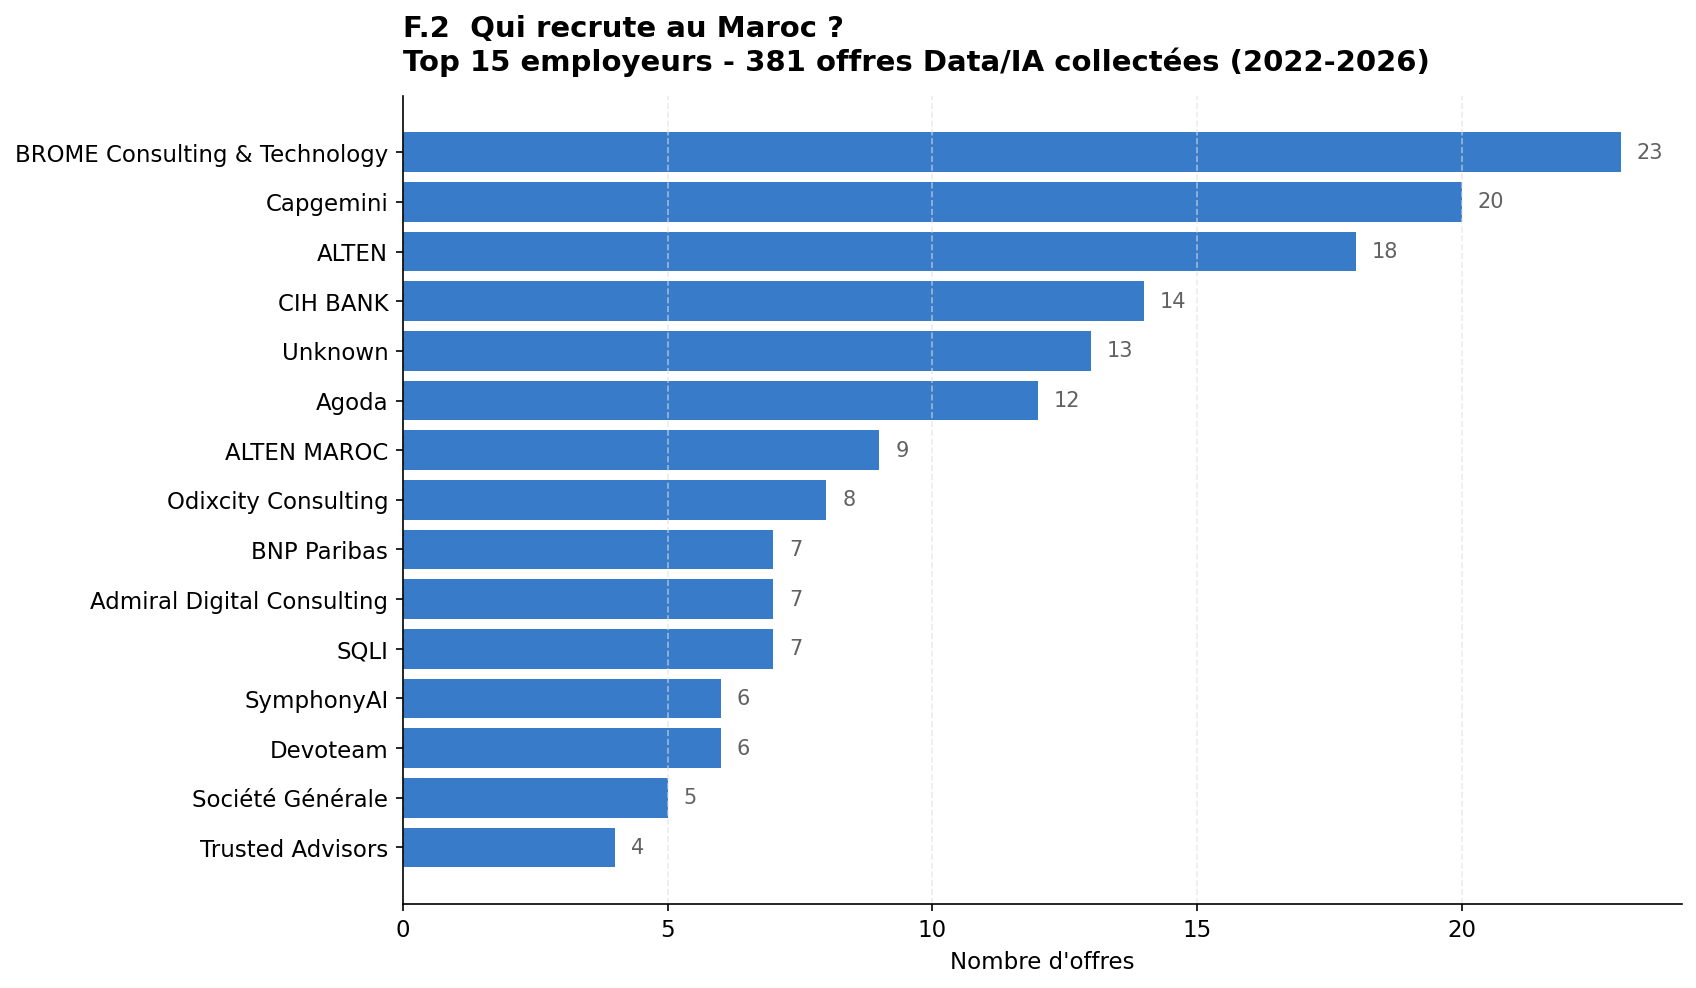
\includegraphics[width=\textwidth]{f02_top_employeurs_maroc.png}
    \caption{Top 15 Maroc.}
  \end{subfigure}\hfill
  \begin{subfigure}[t]{0.48\textwidth}
    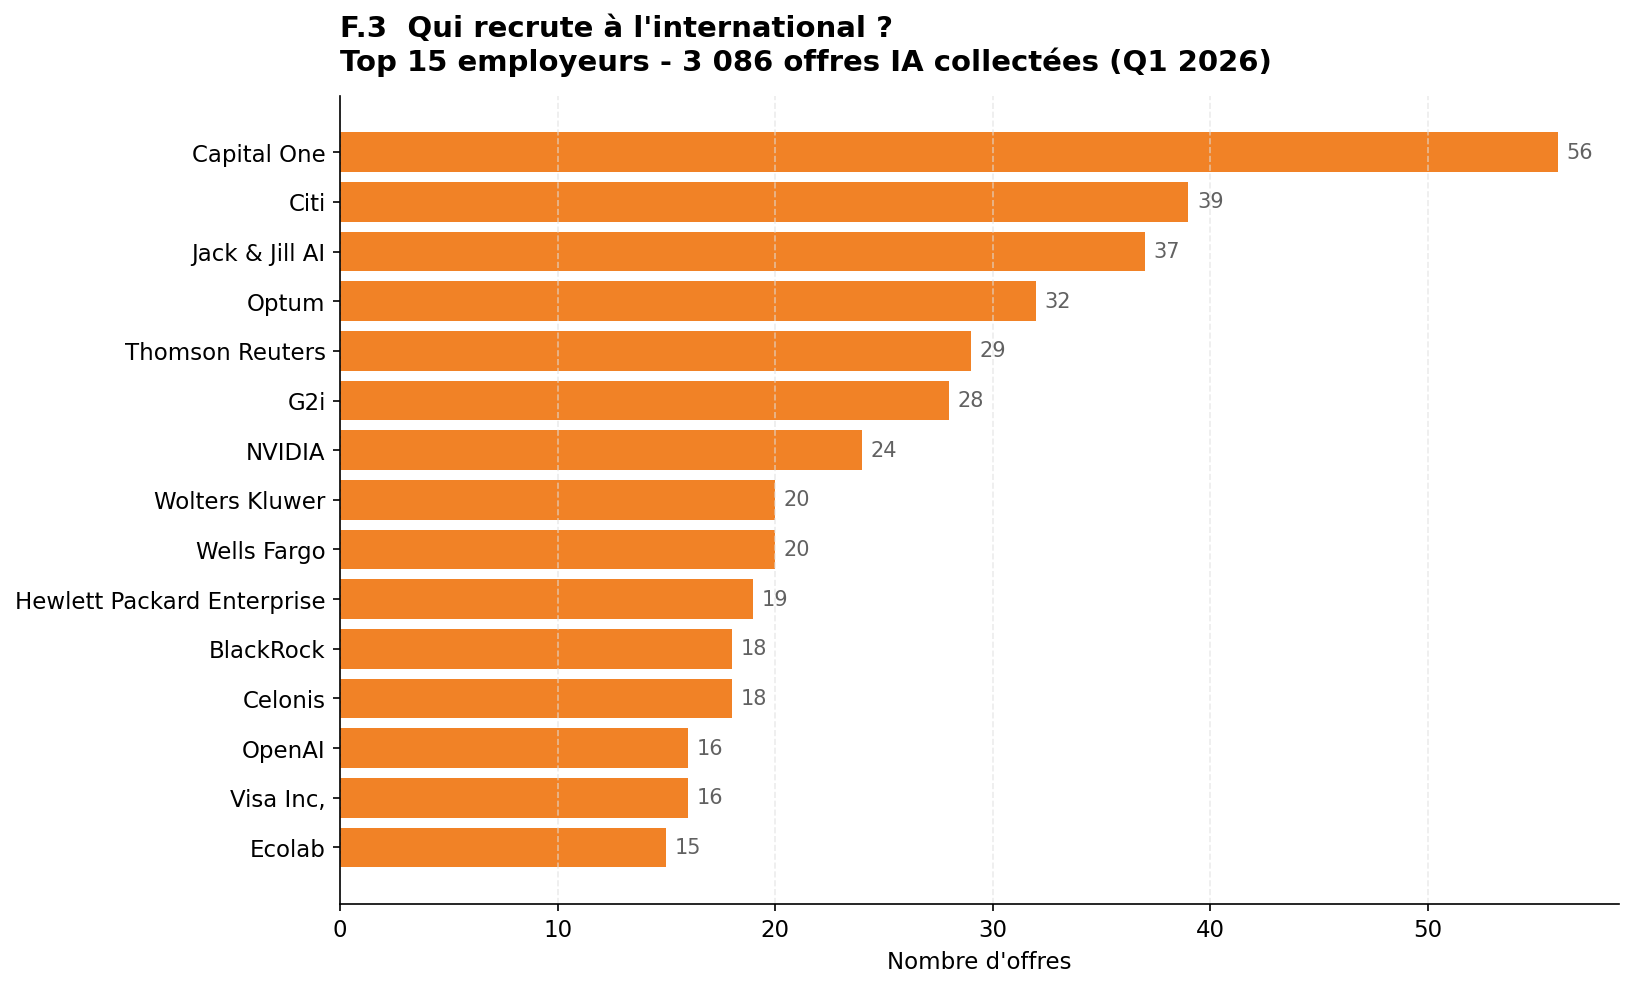
\includegraphics[width=\textwidth]{f03_top_employeurs_intl.png}
    \caption{Top 20 international.}
  \end{subfigure}
  \caption{Top employeurs sur les deux march\'es observ\'es dans le corpus \skillnav.}
  \label{fig:f0203-employeurs}
\end{figure}

\subsection{Top intitul\'es de poste sur les deux march\'es}

La figure~\ref{fig:f1004-intitules}~(a) pr\'esente le top 10 des intitul\'es au Maroc apr\`es canonicalisation. La hi\'erarchie est domin\'ee par les trois intitul\'es classiques du domaine : Data Analyst (37 offres), Data Scientist (30 offres) et Data Engineer (23 offres). Les intitul\'es sp\'ecifiques \`a l'Intelligence Artificielle g\'en\'erative apparaissent \`a des fr\'equences faibles : 4 offres pour AI Engineer, 4 offres pour BI Analyst et seulement 3 offres pour des intitul\'es hybrides du type AI Machine Learning Optimization Engineer.

\`A l'international (figure~\ref{fig:f1004-intitules}~(b)), le top 10 confirme la pr\'epond\'erance des profils AI-First. L'intitul\'e AI Engineer concentre 148 offres et ses d\'eclinaisons hi\'erarchiques (Senior AI Engineer 98, Lead AI Engineer 29, Staff AI Engineer 27, Principal AI Engineer 22) traduisent l'existence de fili\`eres d'\'evolution compl\`etes au sein des entreprises. L'intitul\'e Applied AI Engineer (45 offres) caract\'erise un profil interm\'ediaire d\'edi\'e \`a la mise en production de solutions construites sur des mod\`eles de fondation existants. L'absence d'intitul\'es de type Data Analyst dans le top 10 international tranche avec la composition observ\'ee au Maroc.

\begin{figure}[H]
  \centering
  \begin{subfigure}[t]{0.48\textwidth}
    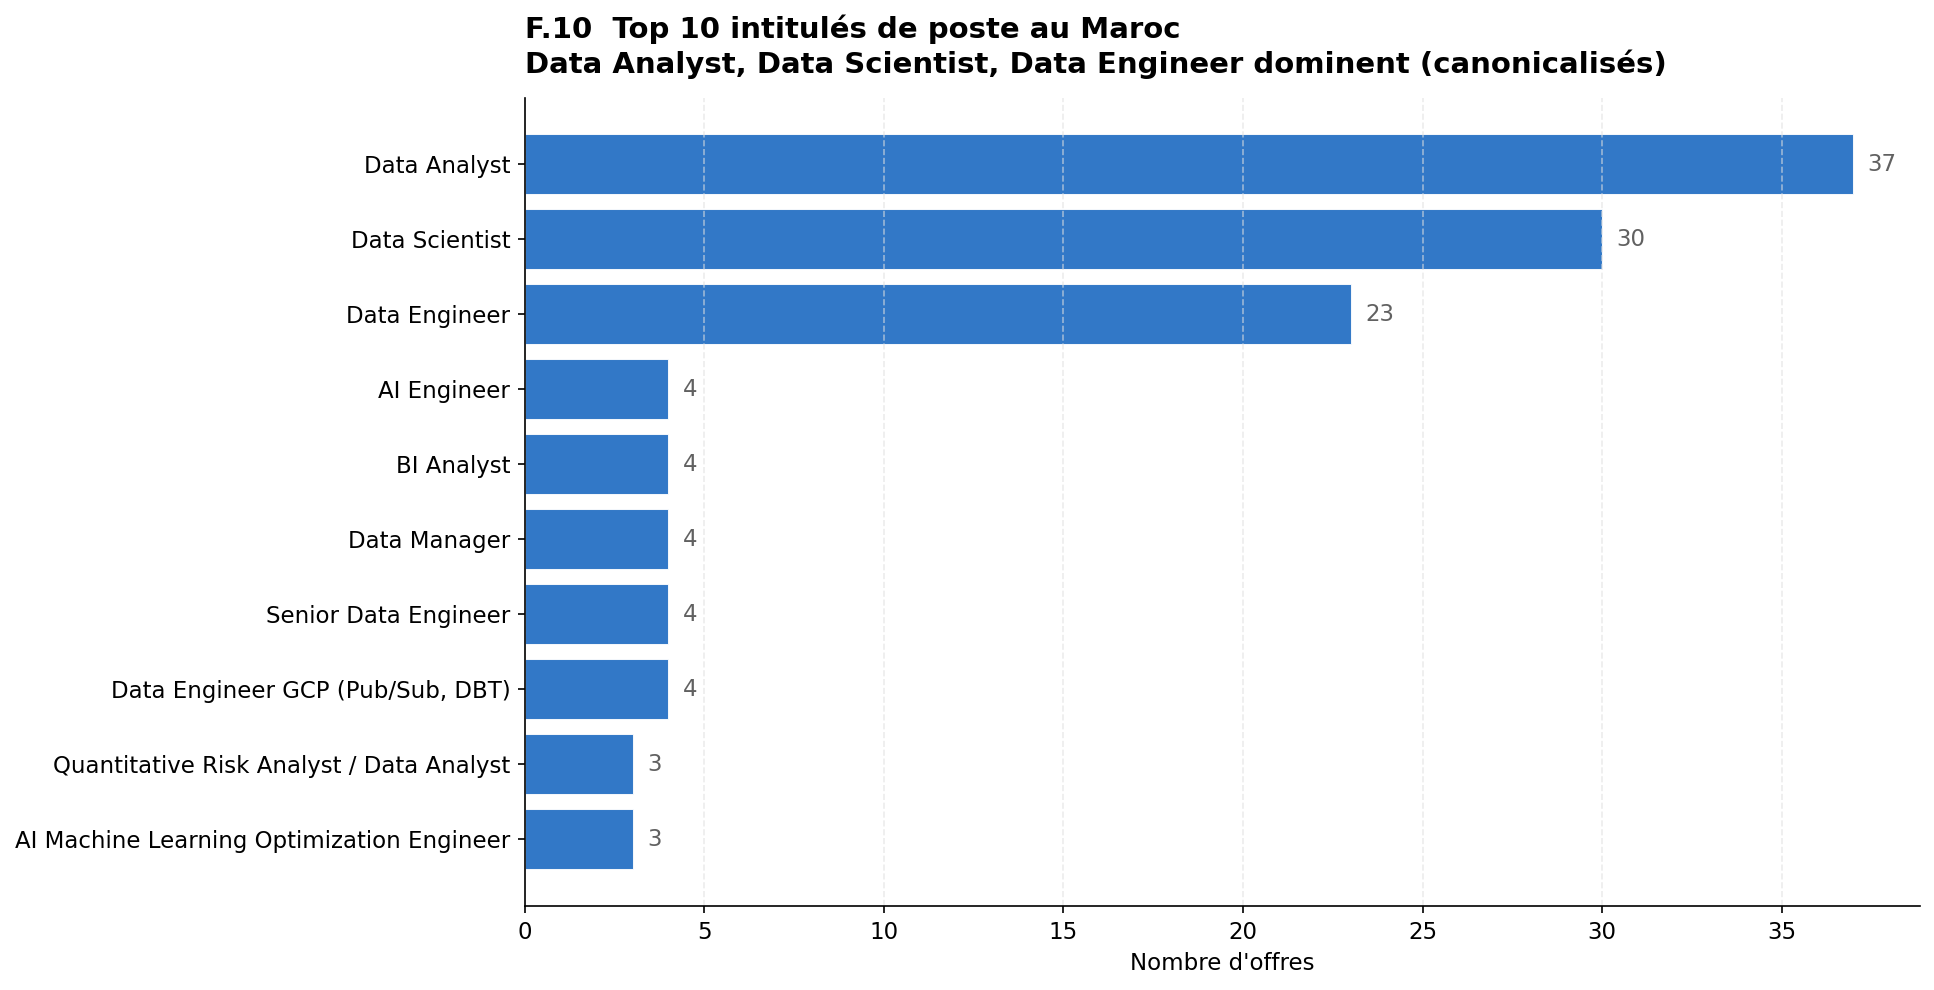
\includegraphics[width=\textwidth]{f10_top_intitules_maroc.png}
    \caption{Top 10 Maroc.}
  \end{subfigure}\hfill
  \begin{subfigure}[t]{0.48\textwidth}
    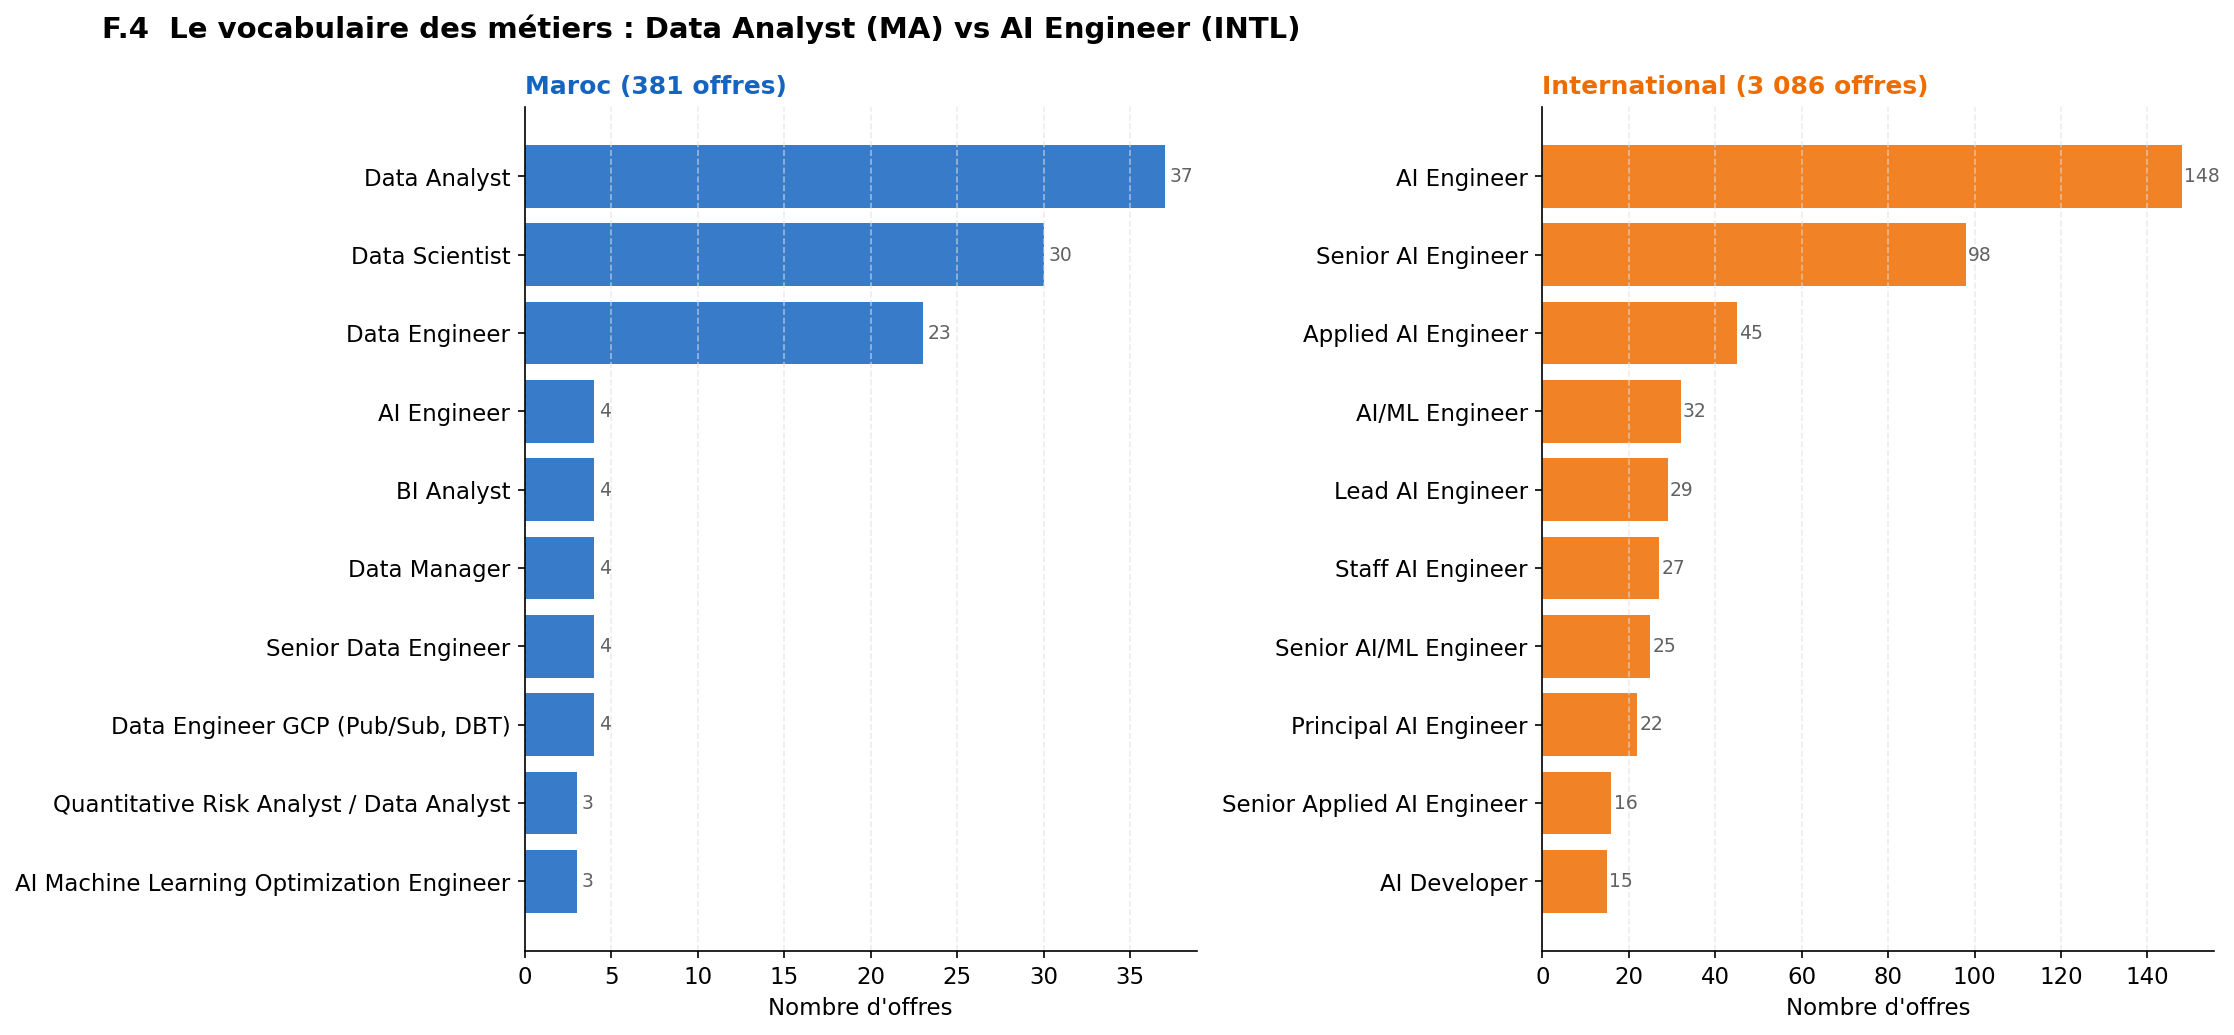
\includegraphics[width=\textwidth]{f04_top_intitules.png}
    \caption{Top 10 international.}
  \end{subfigure}
  \caption{Top 10 des intitul\'es de poste canonicalis\'es sur les deux march\'es.}
  \label{fig:f1004-intitules}
\end{figure}

\section{Comp\'etences par famille}

L'analyse des comp\'etences est conduite sur les dix familles d\'efinies par la taxonomie \skillnav (Intelligence Artificielle g\'en\'erative, Machine Learning, Bases de donn\'ees, Data Engineering, Cloud, Operations et MLOps, Langages de programmation, Frameworks web et APIs, Domaines m\'etier, Autres outils). Le d\'etail de la taxonomie est document\'e dans le module \texttt{skillnav/pipelines/structure\_mining/graph\_builder.py} et reproduit en annexe~A.

\subsection{Comp\'etences dominantes au Maroc}

Les figures~\ref{fig:f11-skills-ma} et~\ref{fig:f12-fam-ma} mettent en \'evidence un profil caract\'eristique du march\'e marocain. Le langage Python (52,8\,\% du corpus marocain) et la ma\^itrise de SQL (57,2\,\%) y constituent les deux comp\'etences les plus universellement demand\'ees. Les outils de Business Intelligence occupent une place significative, avec Power BI \`a 27,6\,\%, Tableau \`a 15,7\,\% et Excel \`a 10,8\,\%. Le Machine Learning classique repr\'esent\'e par scikit-learn (6,6\,\%), TensorFlow (9,4\,\%), PyTorch (9,2\,\%) et Deep Learning (7,6\,\%) confirme la maturit\'e du march\'e sur les techniques ant\'erieures \`a la vague Intelligence Artificielle g\'en\'erative. \`A l'inverse, les comp\'etences caract\'eristiques de l'Intelligence Artificielle g\'en\'erative apparaissent \`a des fr\'equences tr\`es faibles : Large Language Model \`a 6,0\,\%, GenAI \`a 5,0\,\%, RAG \`a 2,9\,\%, LangChain \`a 1,0\,\%.

\begin{figure}[H]
  \centering
  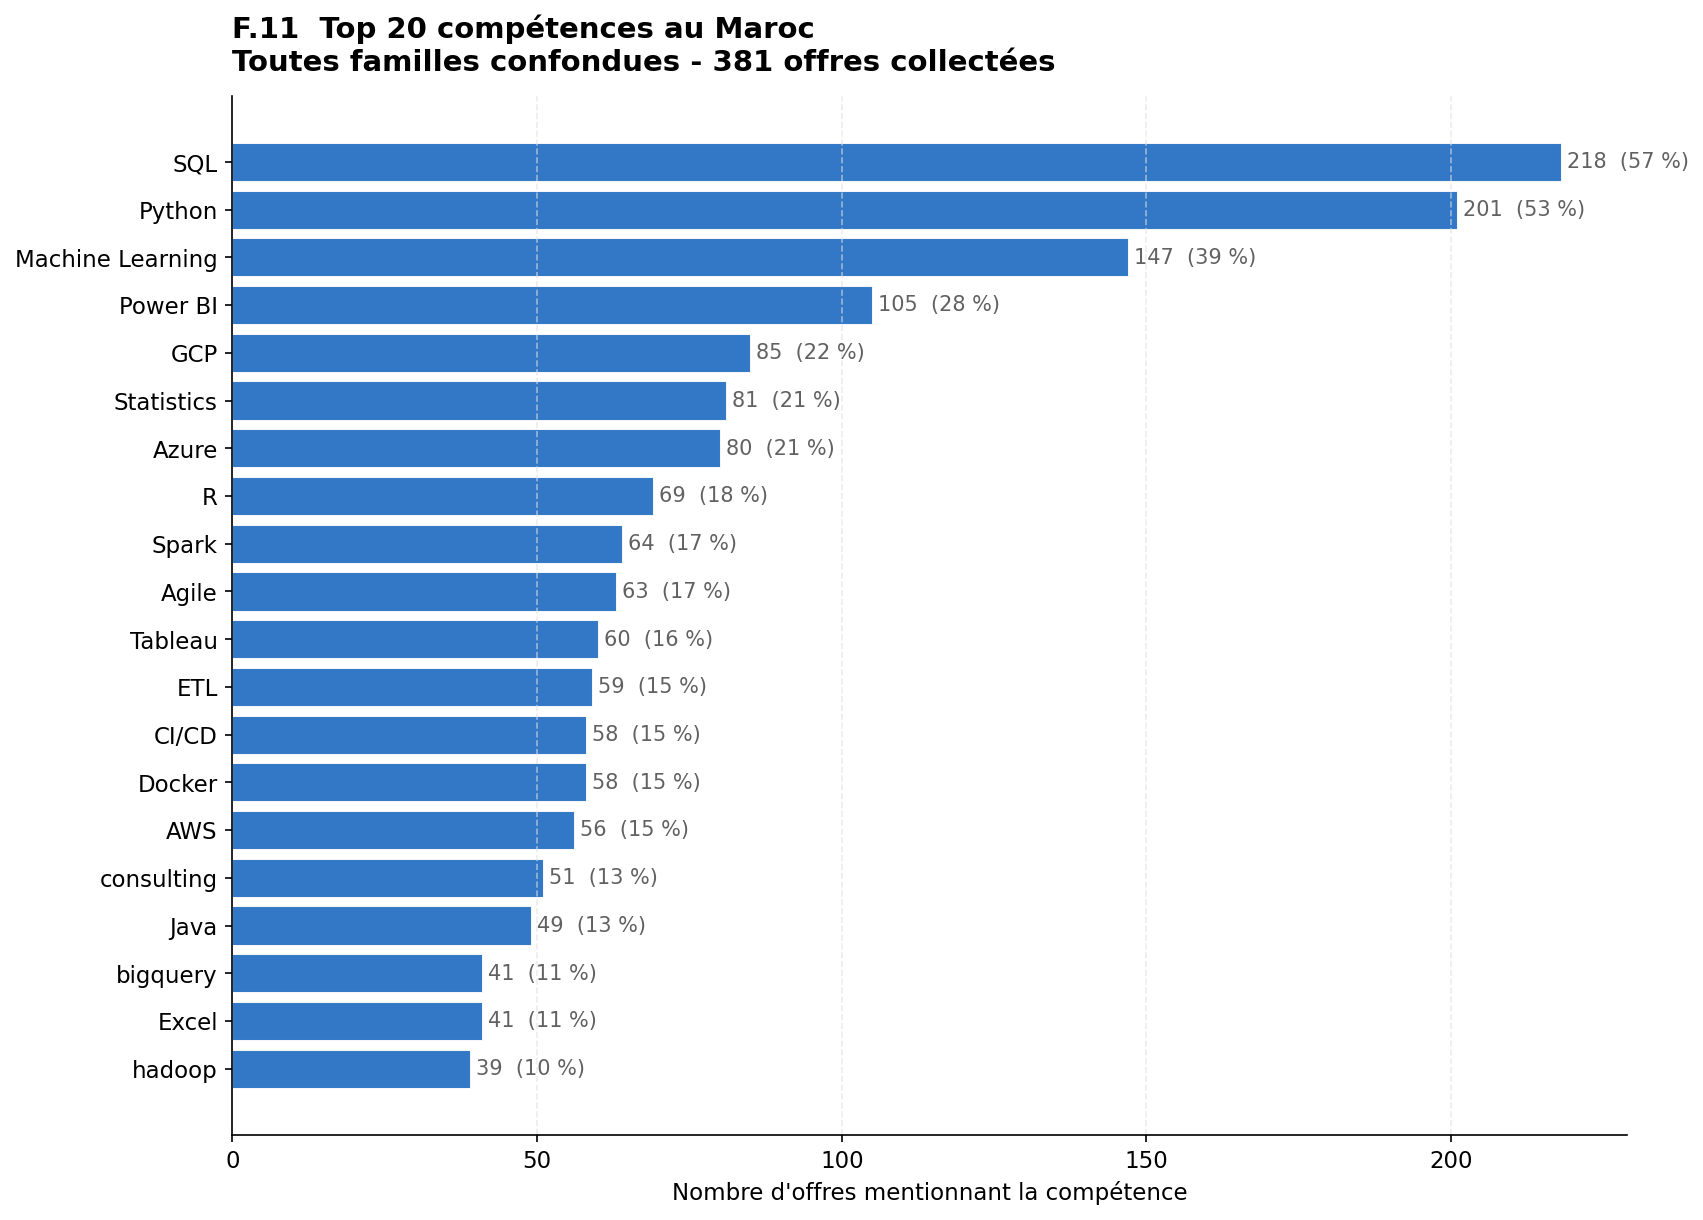
\includegraphics[width=0.82\textwidth]{f11_top_skills_maroc.png}
  \caption{Top 30 des comp\'etences au Maroc, toutes familles confondues.}
  \label{fig:f11-skills-ma}
\end{figure}

\begin{figure}[H]
  \centering
  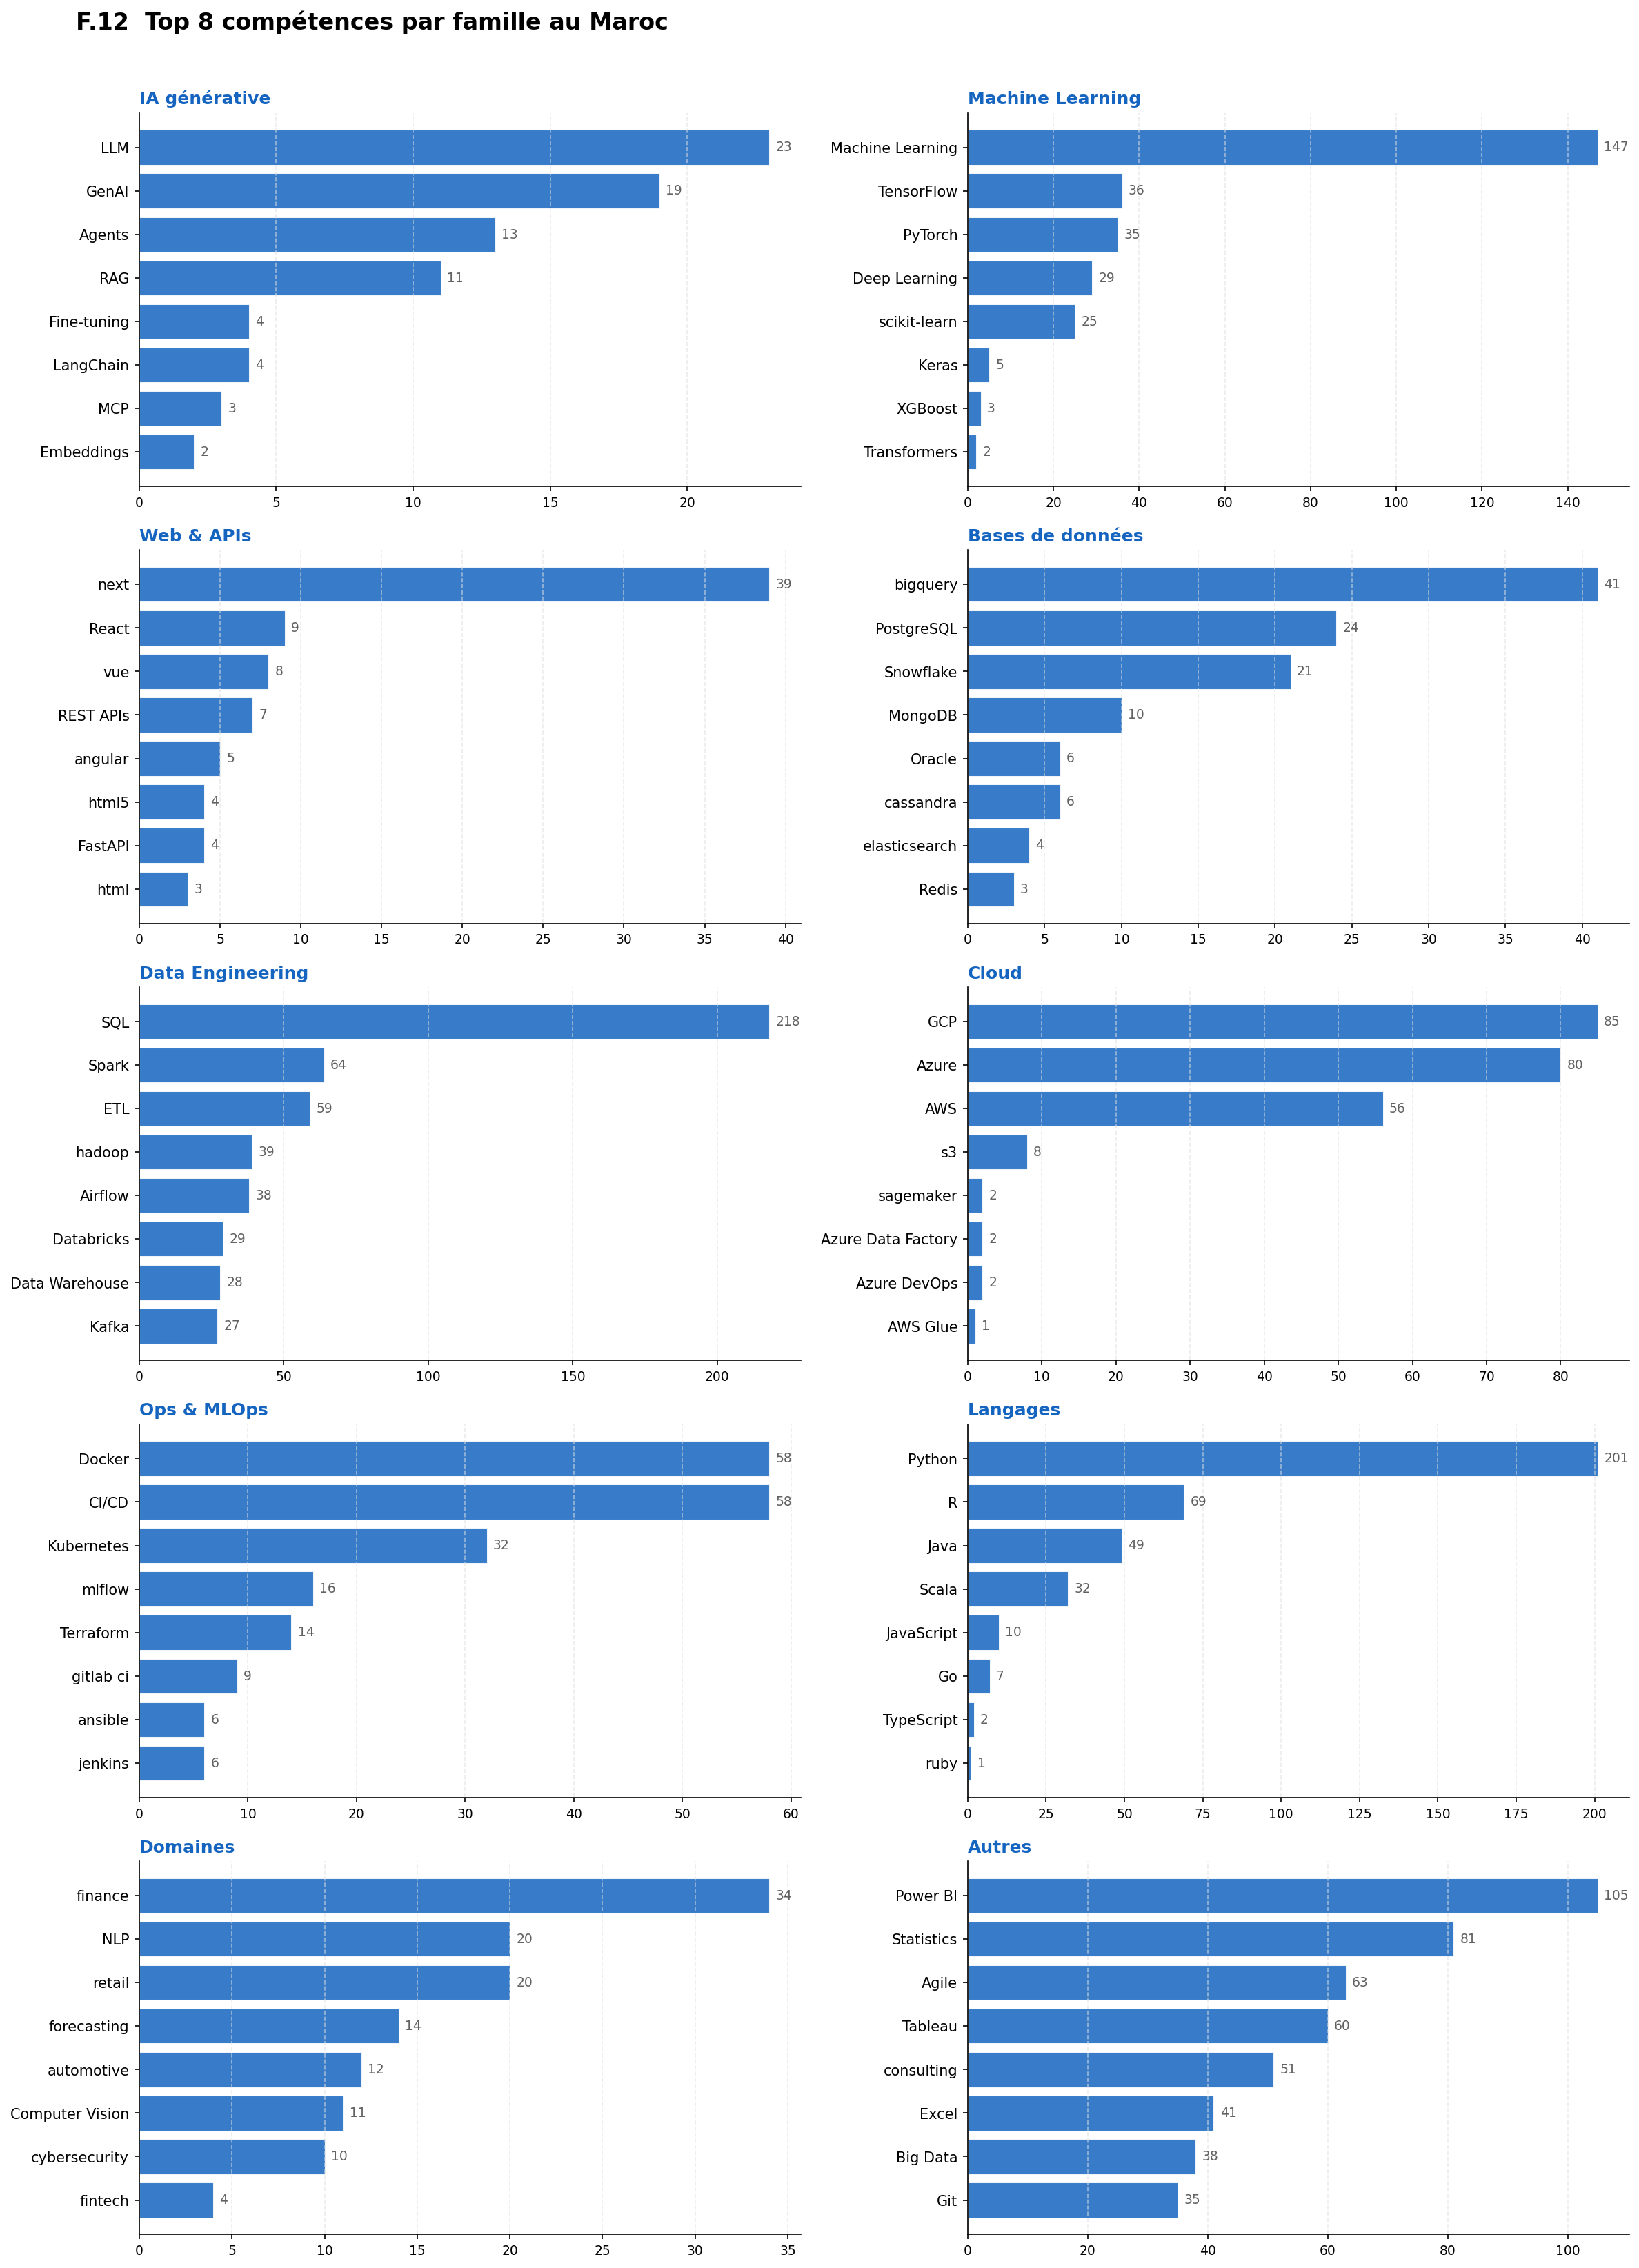
\includegraphics[width=0.85\textwidth]{f12_competences_par_famille_maroc.png}
  \caption{Top 8 des comp\'etences par famille au Maroc.}
  \label{fig:f12-fam-ma}
\end{figure}

\subsection{Comp\'etences dominantes \`a l'international}

Les figures~\ref{fig:f14-skills-intl} et~\ref{fig:f15-fam-intl} dressent un portrait diam\'etralement oppos\'e. Le langage Python s'impose comme une comp\'etence quasi universelle (83,4\,\% du corpus international). Les comp\'etences caract\'eristiques de l'Intelligence Artificielle g\'en\'erative dominent les fr\'equences : Prompt Engineering \`a 37,2\,\%, RAG \`a 34,1\,\%, LangChain \`a 23,4\,\%, Agents \`a 22,6\,\%, Large Language Model \`a 22,6\,\%. La cloud computing fait apparaitre une avance nette d'Amazon Web Services (40,6\,\%) sur Microsoft Azure (28,0\,\%) et Google Cloud Platform (27,4\,\%). Les pratiques d'industrialisation y sont fortement repr\'esent\'ees avec Docker (35,0\,\%), CI/CD (33,7\,\%) et Kubernetes (28,5\,\%).

\begin{figure}[H]
  \centering
  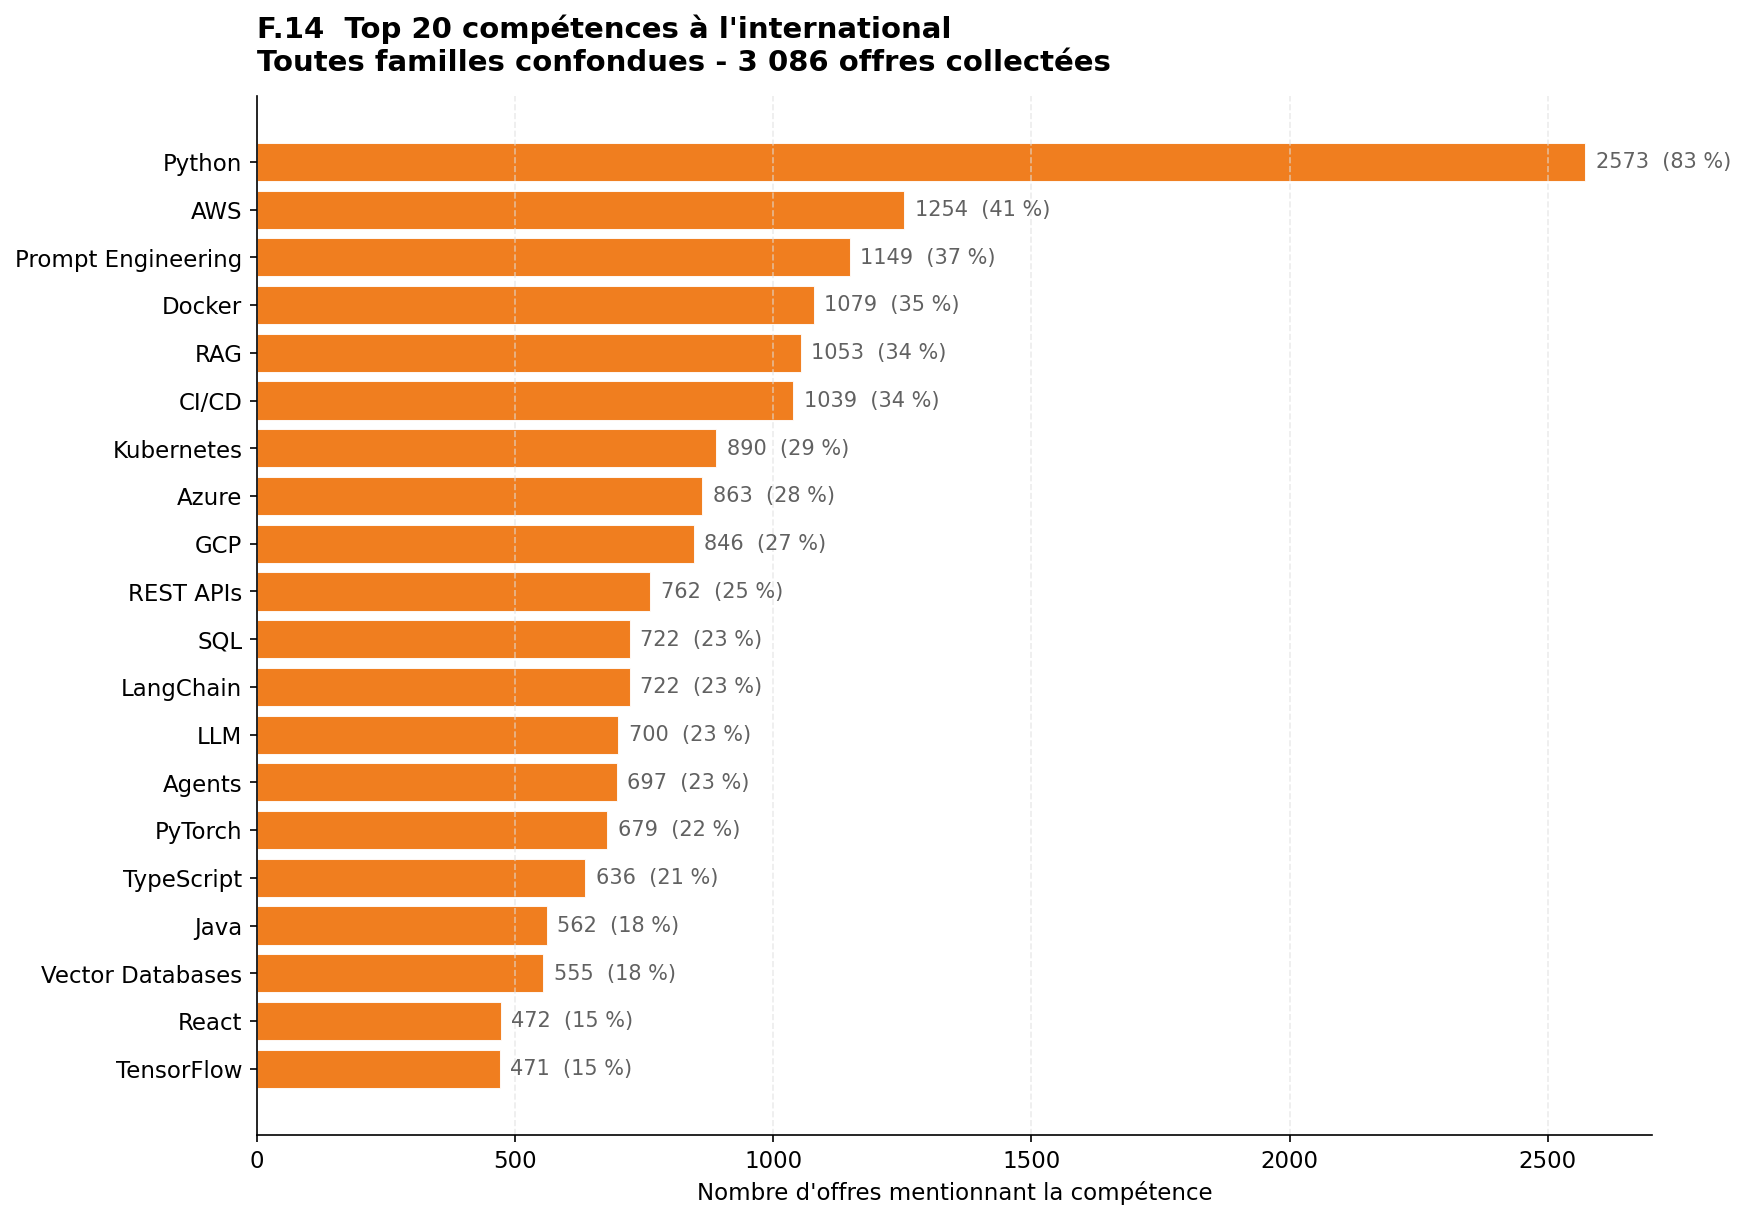
\includegraphics[width=0.82\textwidth]{f14_top_skills_intl.png}
  \caption{Top 30 des comp\'etences \`a l'international, toutes familles confondues.}
  \label{fig:f14-skills-intl}
\end{figure}

\begin{figure}[H]
  \centering
  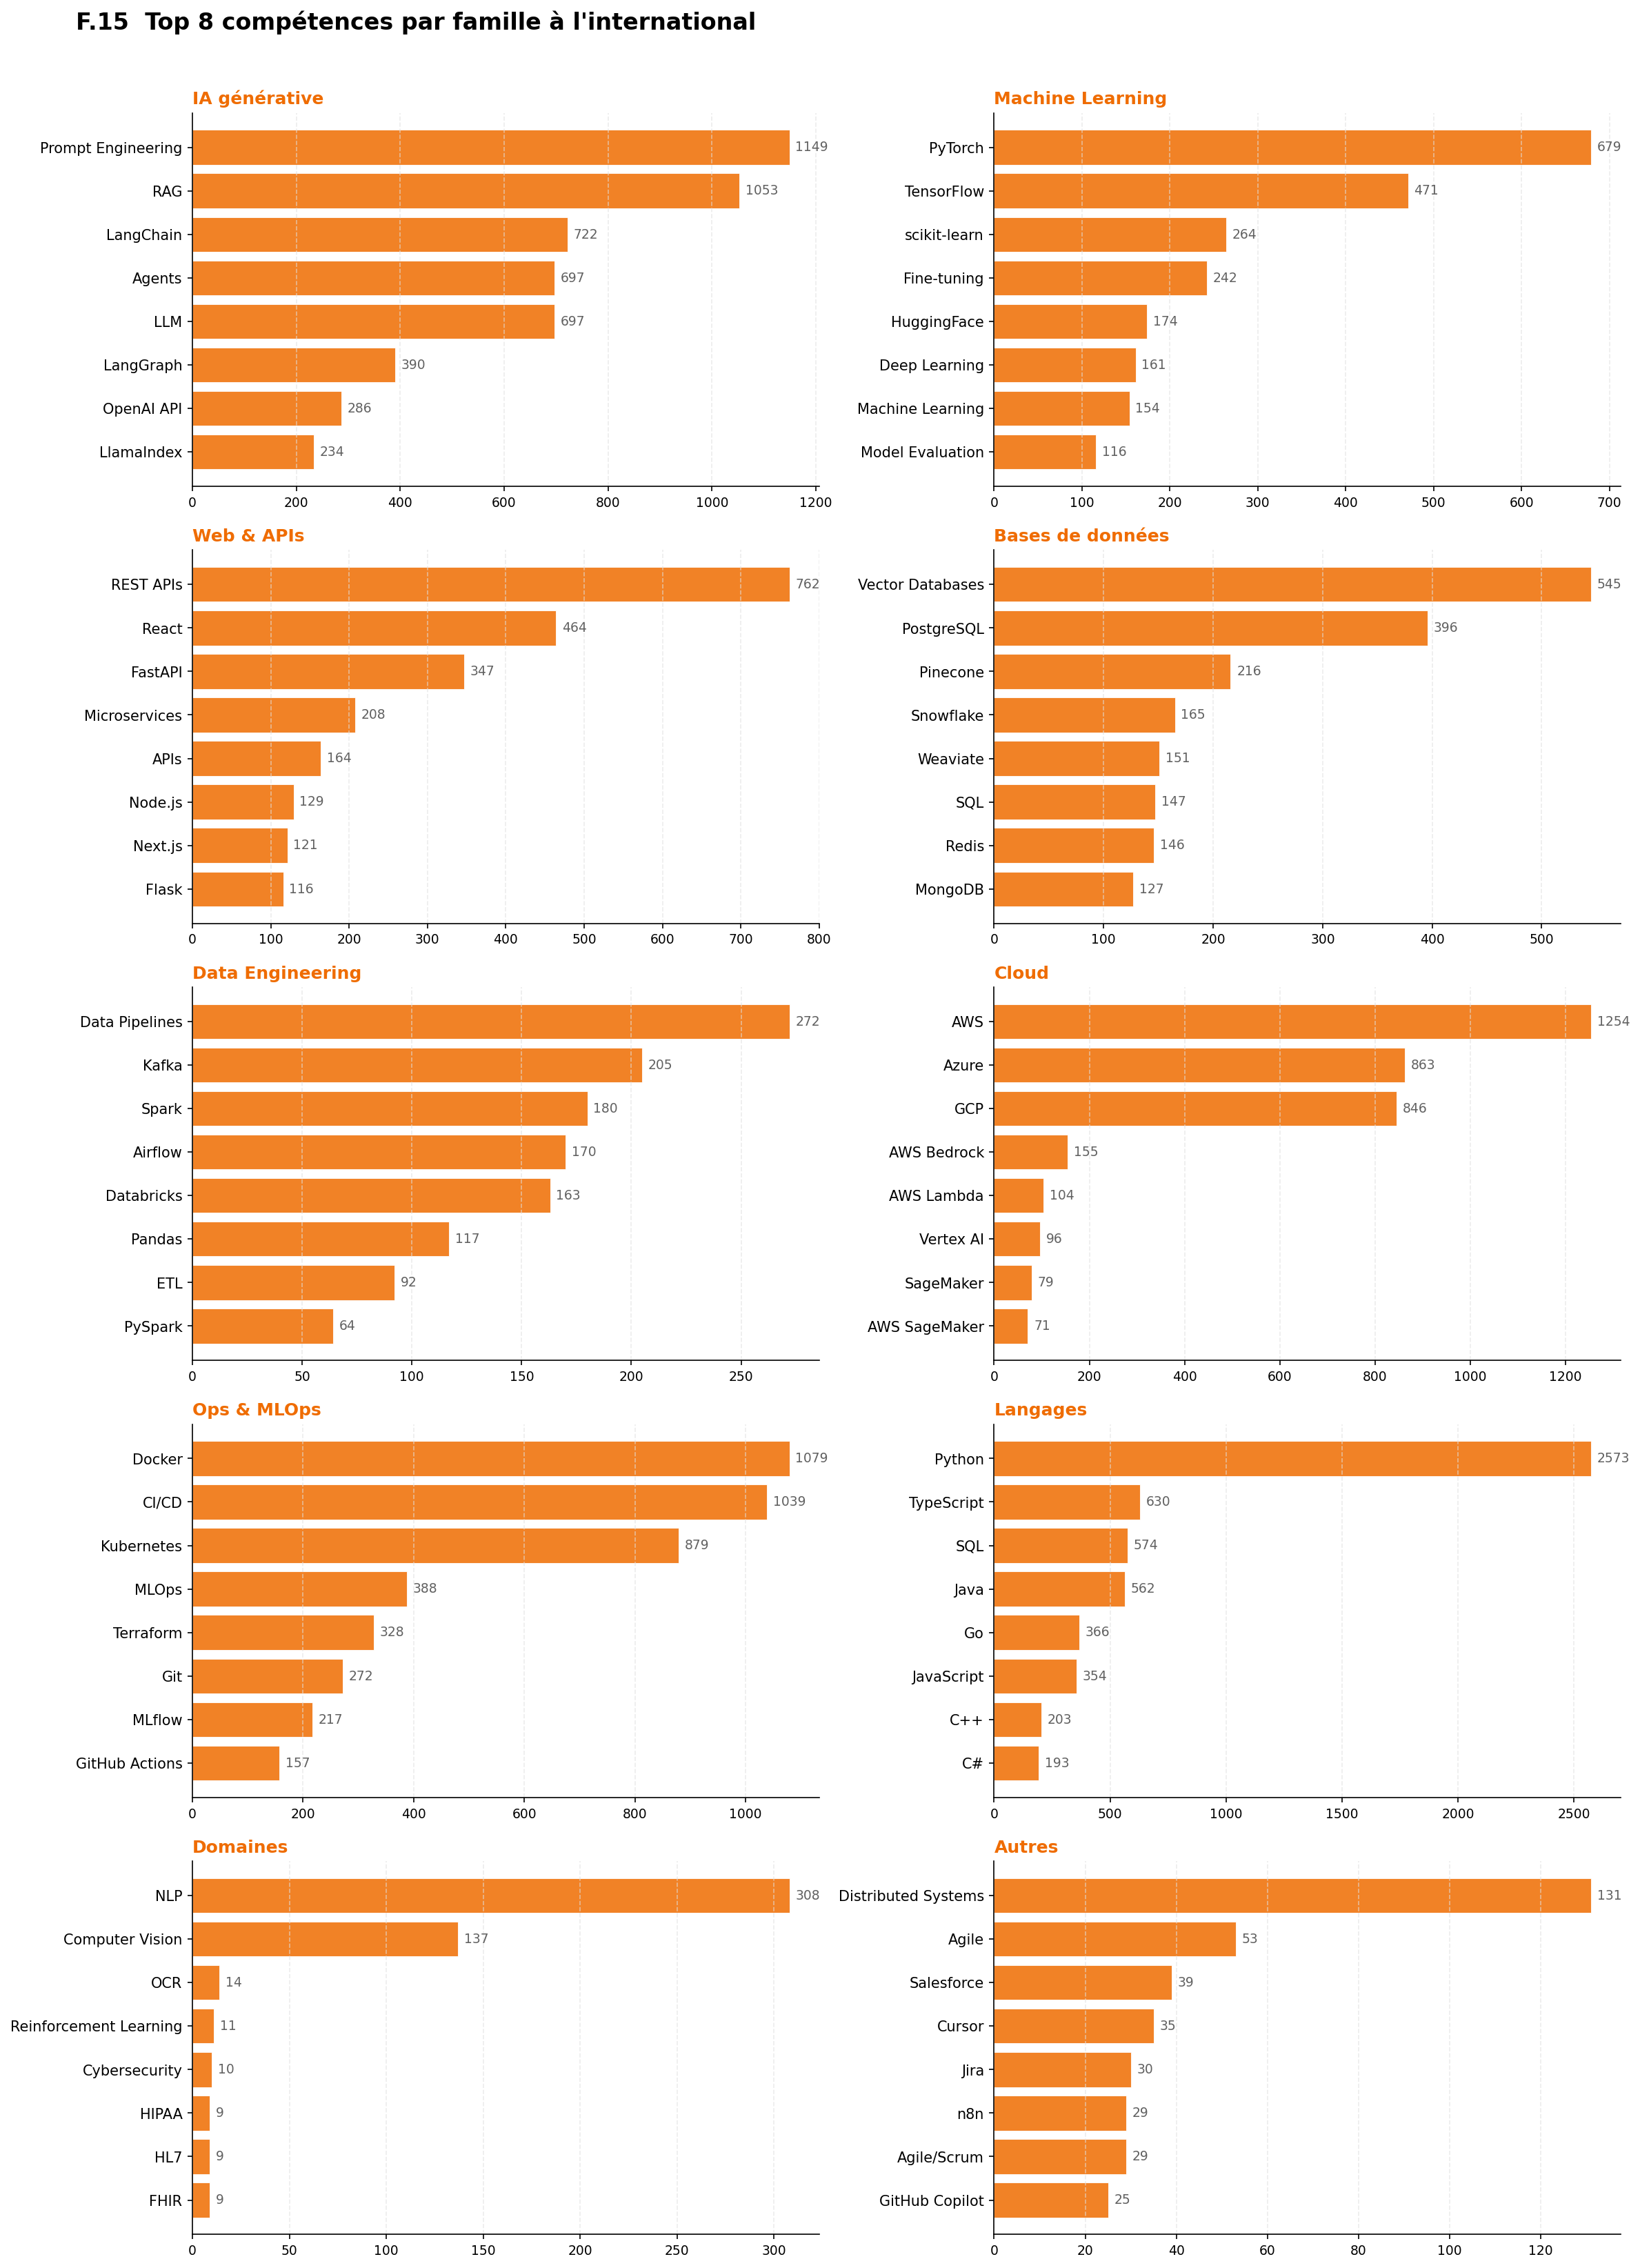
\includegraphics[width=0.85\textwidth]{f15_competences_par_famille_intl.png}
  \caption{Top 10 des comp\'etences par famille \`a l'international.}
  \label{fig:f15-fam-intl}
\end{figure}

\section{\'Ecosyst\`eme des frameworks d'Intelligence Artificielle g\'en\'erative}

L'examen cibl\'e des frameworks d'orchestration d'Intelligence Artificielle g\'en\'erative r\'ev\`ele un \'ecart de maturit\'e consid\'erable entre les deux march\'es. Au Maroc, seuls LangChain (4 offres, 1,0\,\%) et LlamaIndex (1 offre, 0,3\,\%) sont mentionn\'es explicitement. \`A l'international, l'\'ecosyst\`eme est nettement plus diversifi\'e et plus largement adopt\'e, comme illustr\'e par la figure~\ref{fig:f05-genai} : LangChain est cit\'e dans 722 offres (23,4\,\%), LangGraph dans 390 offres (12,6\,\%), LlamaIndex dans 234 offres (7,6\,\%), CrewAI dans 184 offres (6,0\,\%), AutoGen dans 129 offres (4,2\,\%), Semantic Kernel dans 73 offres (2,4\,\%) et Haystack dans 24 offres (0,8\,\%).

\begin{figure}[H]
  \centering
  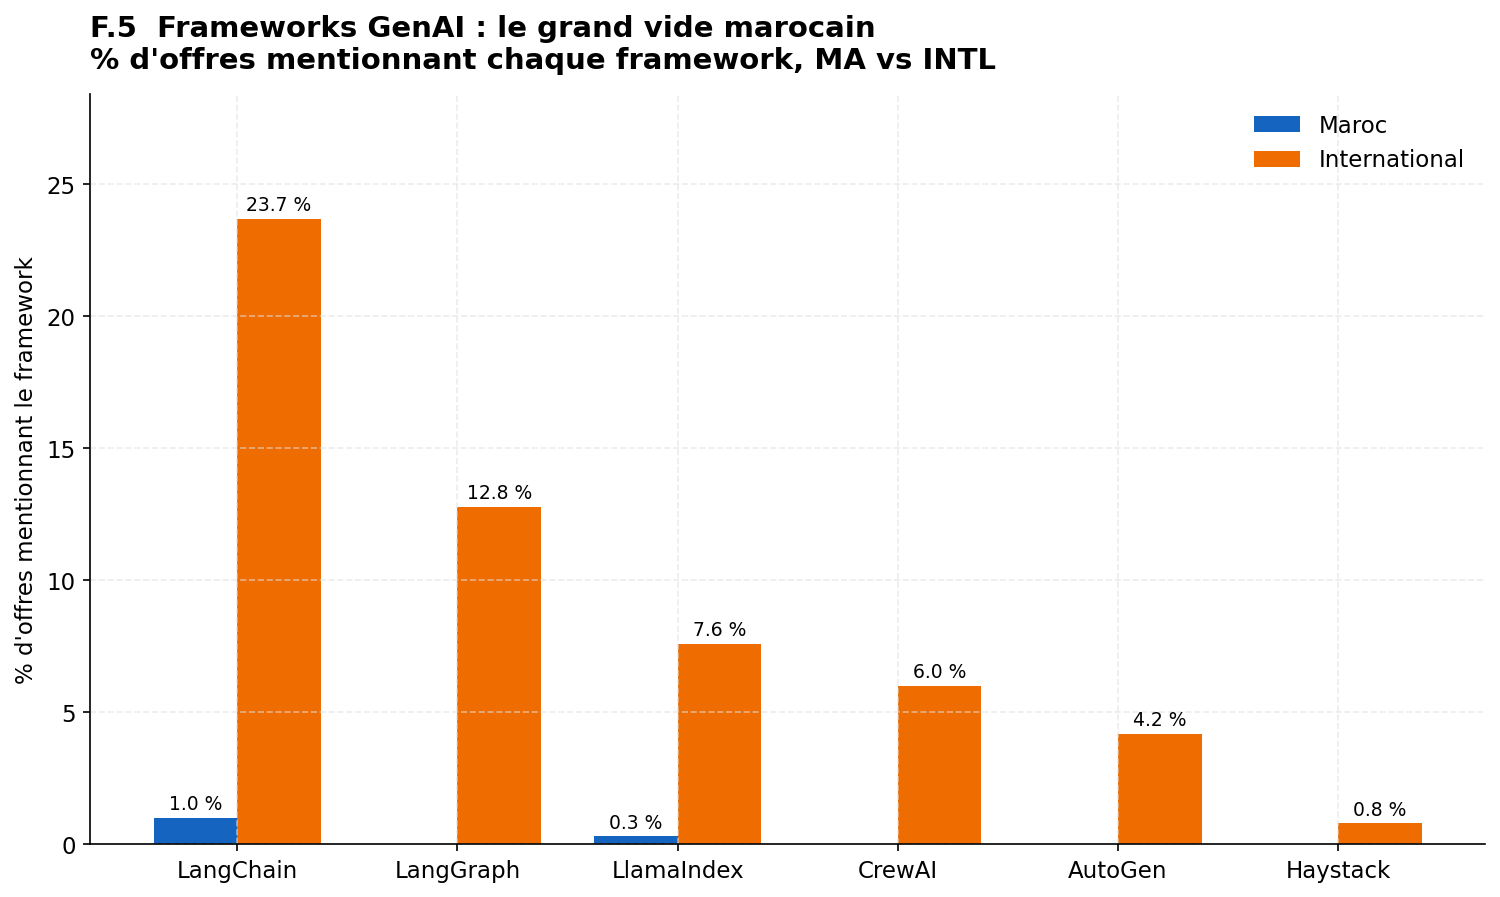
\includegraphics[width=0.82\textwidth]{f05_frameworks_genai.png}
  \caption{\'Ecosyst\`eme des frameworks d'Intelligence Artificielle g\'en\'erative dans le corpus \skillnav.}
  \label{fig:f05-genai}
\end{figure}

L'\'ecart est particuli\`erement saillant pour les frameworks d'orchestration d'agents conversationnels (CrewAI, AutoGen, LangGraph) qui n'apparaissent dans aucune offre marocaine du corpus.

\section{Grand \'ecart de comp\'etences entre march\'e international et march\'e marocain}

L'analyse des dix comp\'etences les plus sur-repr\'esent\'ees \`a l'international par rapport au Maroc, pr\'esent\'ee sur la figure~\ref{fig:f06-ecart}, confirme et quantifie l'\'ecart structurel entre les deux march\'es. L'\'ecart le plus marqu\'e concerne Large Language Model, qui appara\^it dans 54,2\,\% des offres internationales contre seulement 6,3\,\% des offres marocaines, soit un \'ecart de 47,9 points de pourcentage. Suivent RAG (43,5\,\% contre 2,9\,\%, \'ecart de 40,6 points), Prompt Engineering (37,6\,\% contre 0,5\,\%, \'ecart de 37,1 points), Amazon Web Services (46,5\,\% contre 14,7\,\%, \'ecart de 31,8 points) et le langage Python lui-m\^eme (83,4\,\% contre 52,8\,\%, \'ecart de 30,6 points).

\begin{figure}[H]
  \centering
  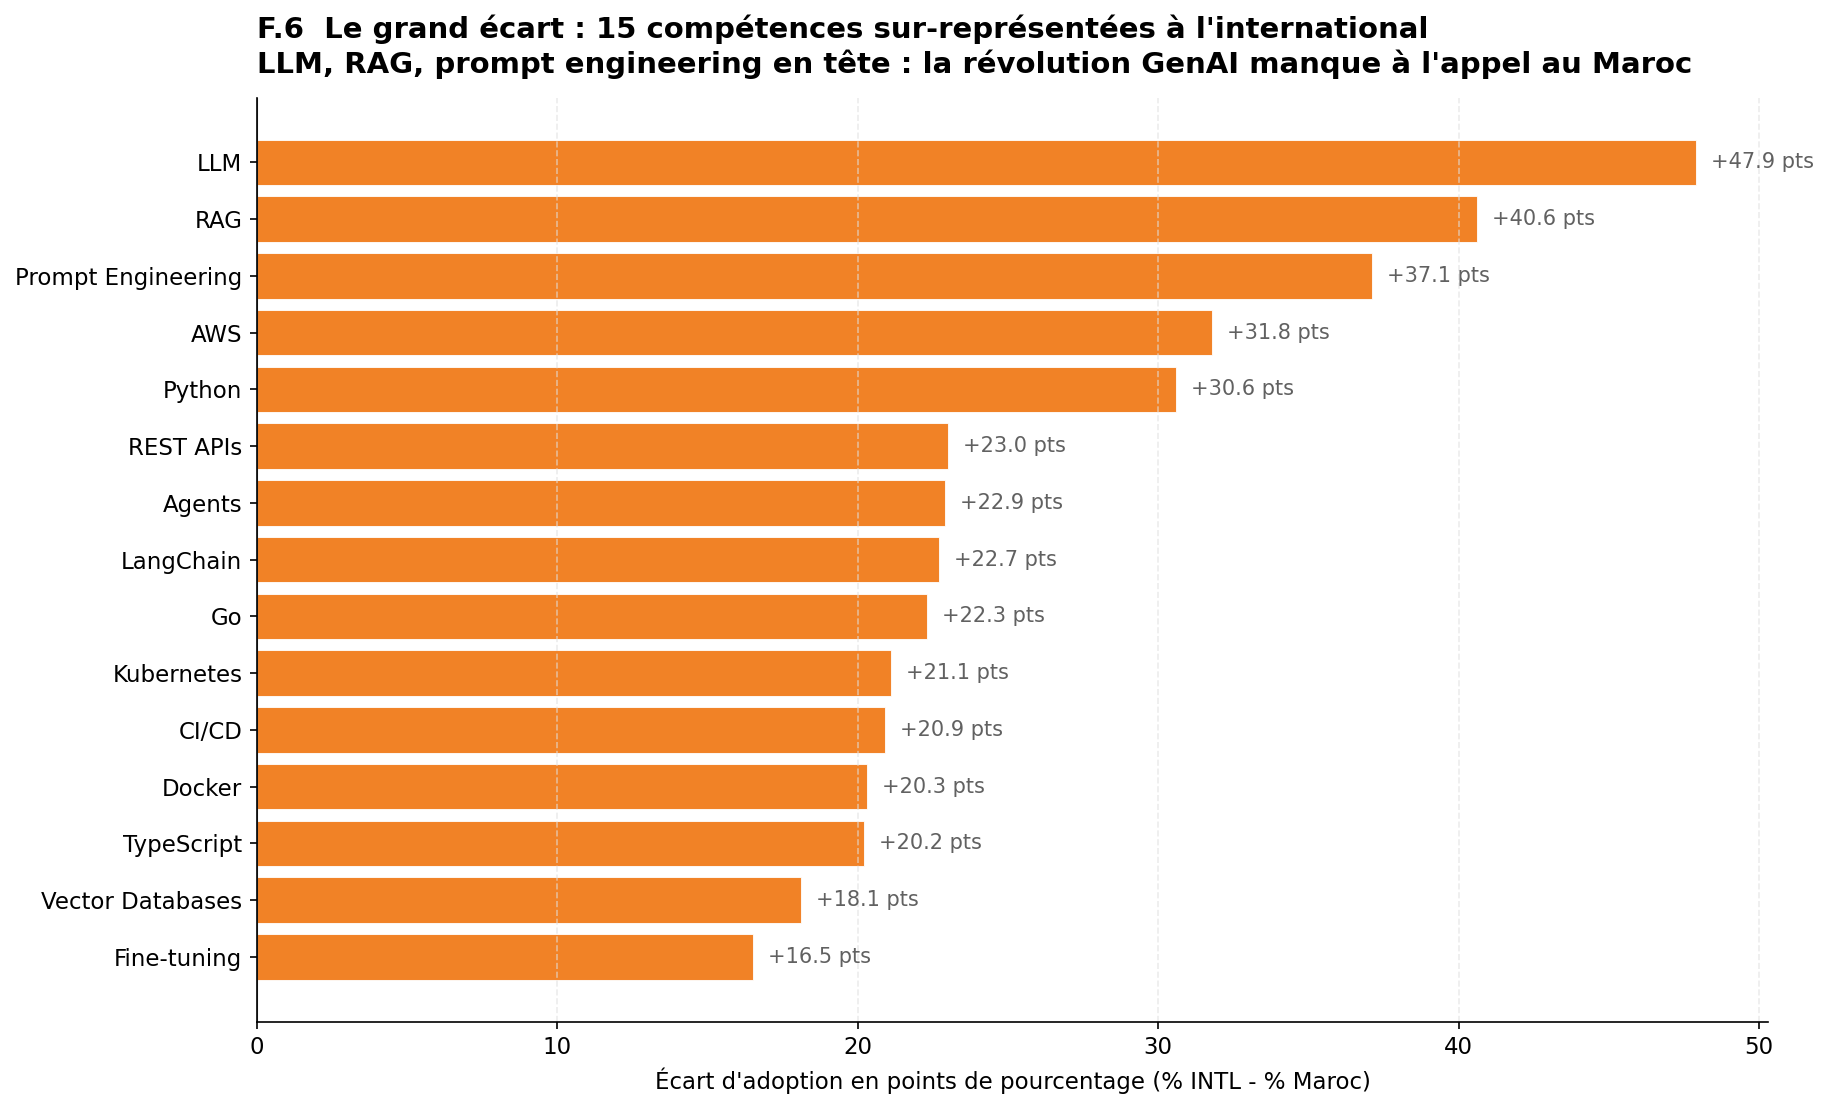
\includegraphics[width=0.82\textwidth]{f06_grand_ecart_intl_vs_ma.png}
  \caption{Top 10 des comp\'etences les plus sur-repr\'esent\'ees \`a l'international par rapport au Maroc.}
  \label{fig:f06-ecart}
\end{figure}

Ces \'ecarts consid\'erables, mesur\'es en points de pourcentage, dessinent un retard d'adoption du Maroc sur les comp\'etences caract\'eristiques de la vague Intelligence Artificielle g\'en\'erative.

\section{Comp\'etences typiques du march\'e marocain}

L'analyse sym\'etrique des comp\'etences sur-repr\'esent\'ees au Maroc par rapport \`a l'international, pr\'esent\'ee sur la figure~\ref{fig:f07-skills-ma}, livre un portrait coh\'erent du march\'e national. La comp\'etence la plus sur-repr\'esent\'ee au Maroc est SQL (59,1\,\% contre 35,3\,\% \`a l'international, \'ecart de 23,8 points). Suivent les outils de Data Engineering classique : Spark (19,2\,\% contre 7,5\,\%, \'ecart de 11,7 points), Airflow (10,0\,\% contre 5,9\,\%, \'ecart de 4,1 points), Databricks (7,6\,\% contre 6,7\,\%). Les outils Microsoft sont \'egalement mieux repr\'esent\'es au Maroc, Power BI atteignant 27,6\,\% du corpus marocain contre 0,8\,\% \`a l'international.

\begin{figure}[H]
  \centering
  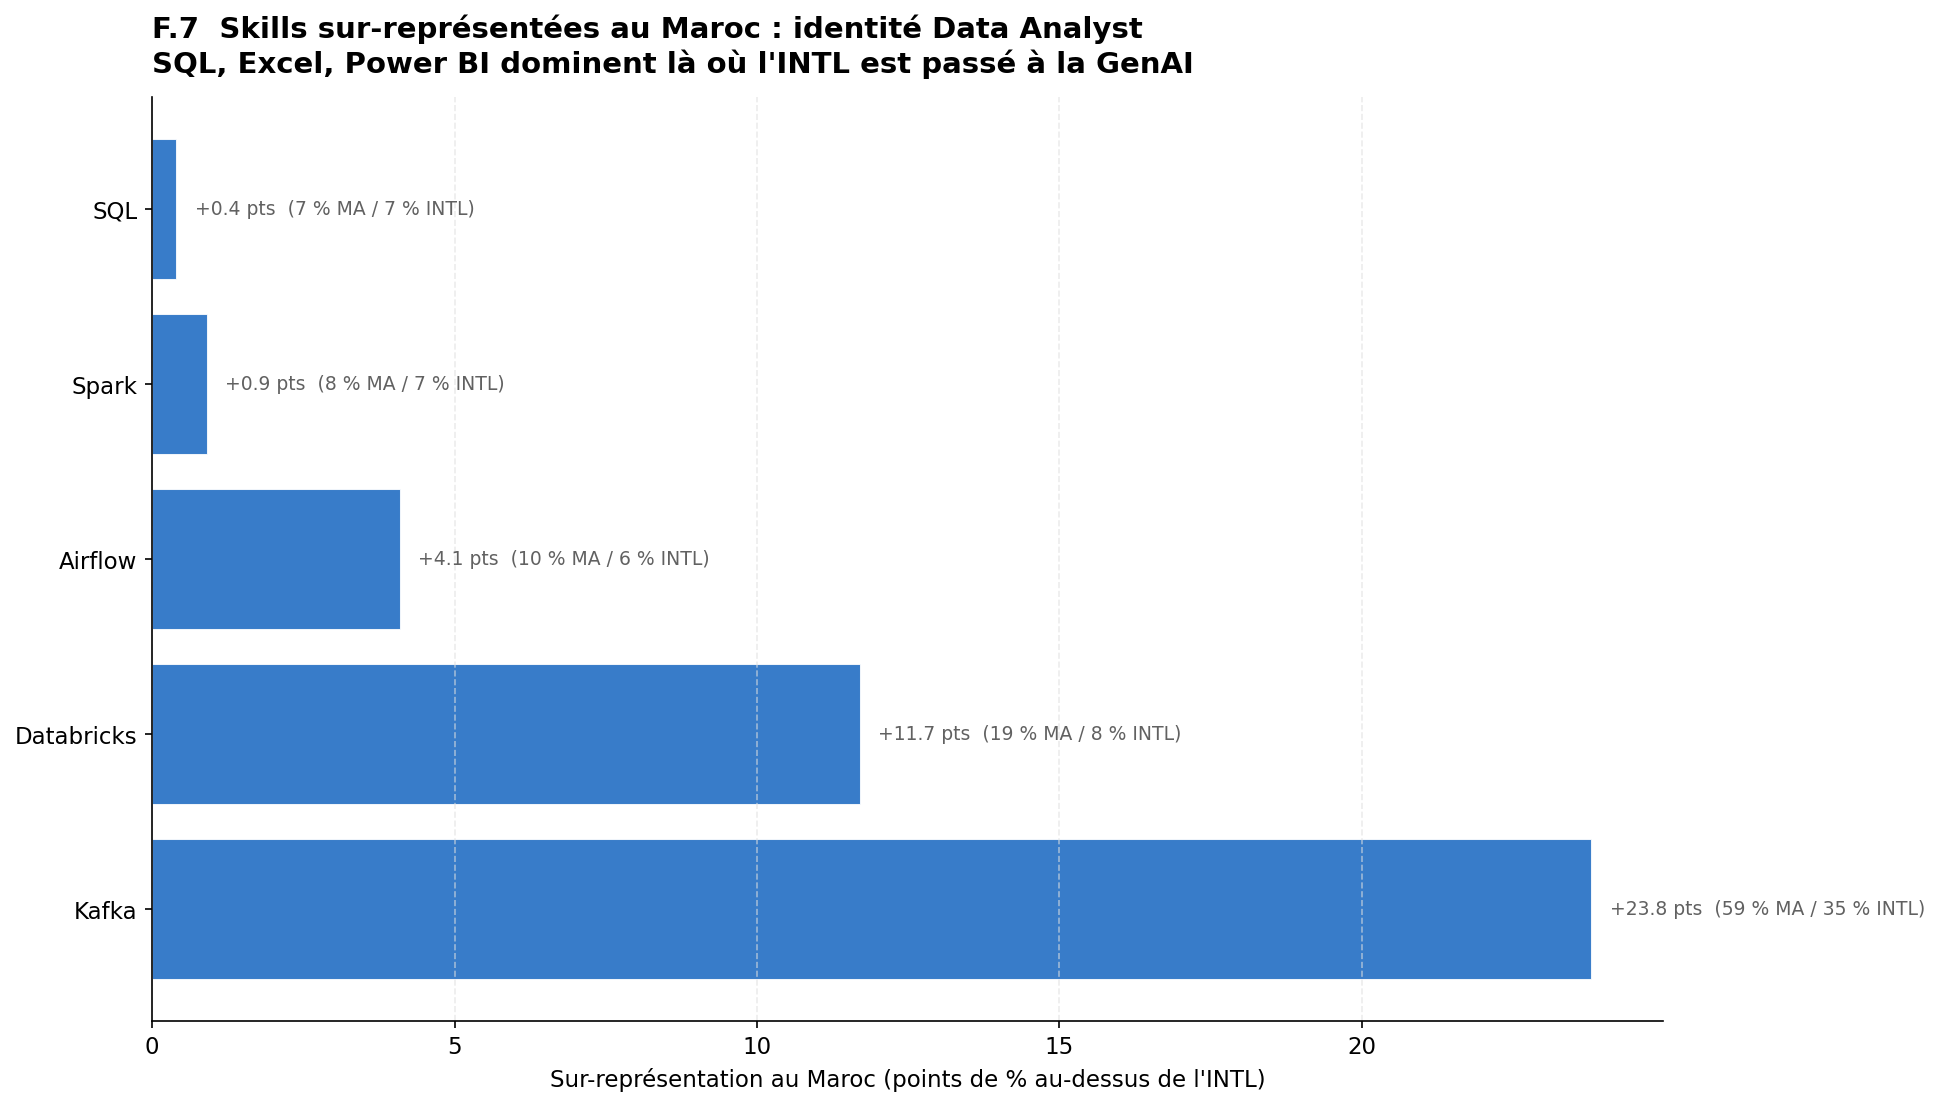
\includegraphics[width=0.82\textwidth]{f07_skills_typiques_maroc.png}
  \caption{Top 10 des comp\'etences les plus sur-repr\'esent\'ees au Maroc par rapport \`a l'international.}
  \label{fig:f07-skills-ma}
\end{figure}

Ce portrait permet de caract\'eriser le march\'e marocain comme un march\'e orient\'e Data Analytics traditionnel et Data Engineering, dans lequel les comp\'etences SQL, les outils de Business Intelligence Microsoft et les frameworks Big Data classiques (Spark, Airflow, Databricks) pr\'edominent.

\section{Profils recherche et profils application ou production}

L'orientation scientifique des profils est estim\'ee \`a partir d'une heuristique de pond\'eration de mots-cl\'es appliqu\'ee au titre et \`a la description des offres. Au Maroc, 70 fiches (18,4\,\%) sont class\'ees comme orient\'ees recherche tandis que 311 fiches (81,6\,\%) sont class\'ees comme orient\'ees application ou production. \`A l'international, l'\'ecart est plus prononc\'e : 94 fiches seulement (3,0\,\%) sont class\'ees comme orient\'ees recherche, contre 2\,992 fiches (97,0\,\%) orient\'ees application ou production.

\begin{figure}[H]
  \centering
  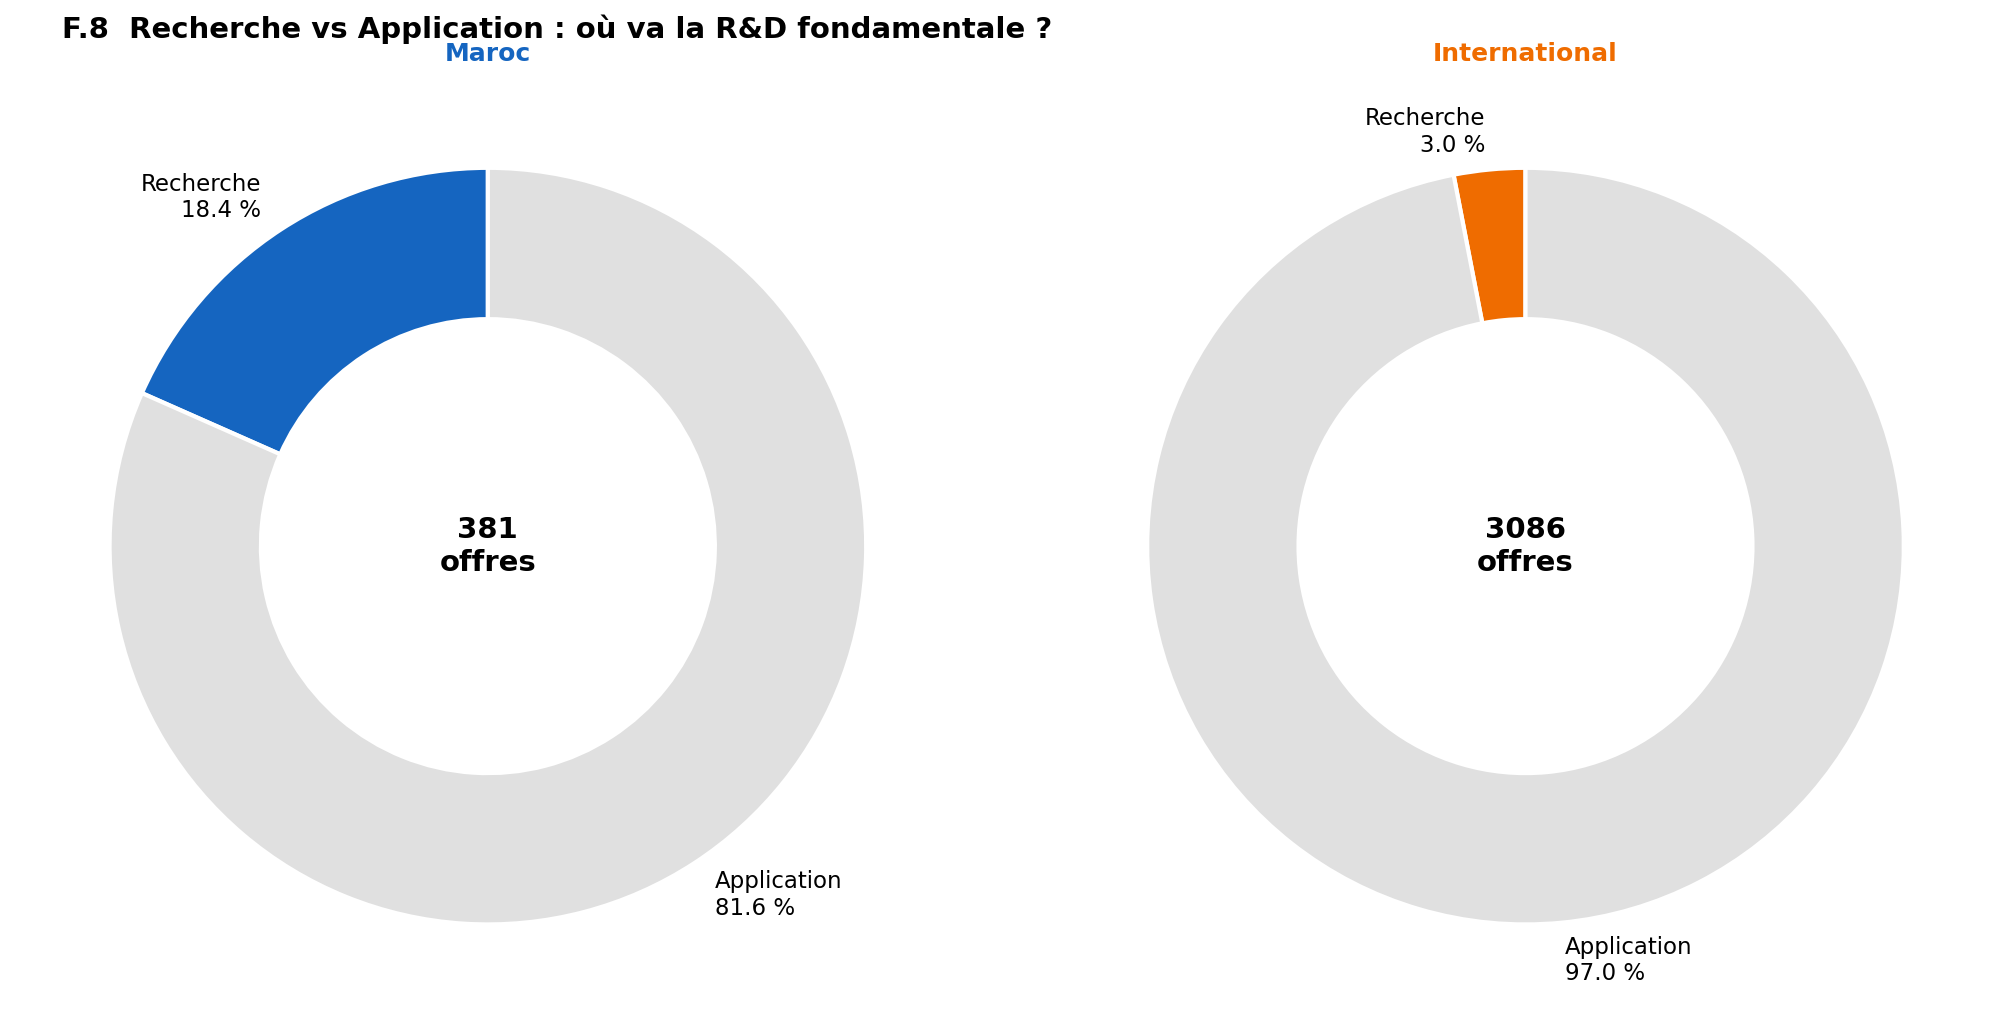
\includegraphics[width=0.78\textwidth]{f08_recherche_vs_applied.png}
  \caption{Distribution des profils recherche et profils application ou production dans les deux corpus.}
  \label{fig:f08-research}
\end{figure}

La quasi-absence de profils d\'edi\'es \`a la recherche dans le corpus international s'explique par la sp\'ecialisation de la source \texttt{builtin.com}, dont le p\'erim\`etre \'editorial concerne essentiellement le march\'e de l'emploi tech industriel et non les laboratoires acad\'emiques ou les centres de recherche.

\section{Comparaison cibl\'ee des vingt premi\`eres comp\'etences}

La comparaison directe des vingt premi\`eres comp\'etences entre les deux corpus, pr\'esent\'ee sur la figure~\ref{fig:f16-top20}, synth\'etise les constats des sections pr\'ec\'edentes. Trois groupes de comp\'etences se d\'egagent.

\begin{figure}[H]
  \centering
  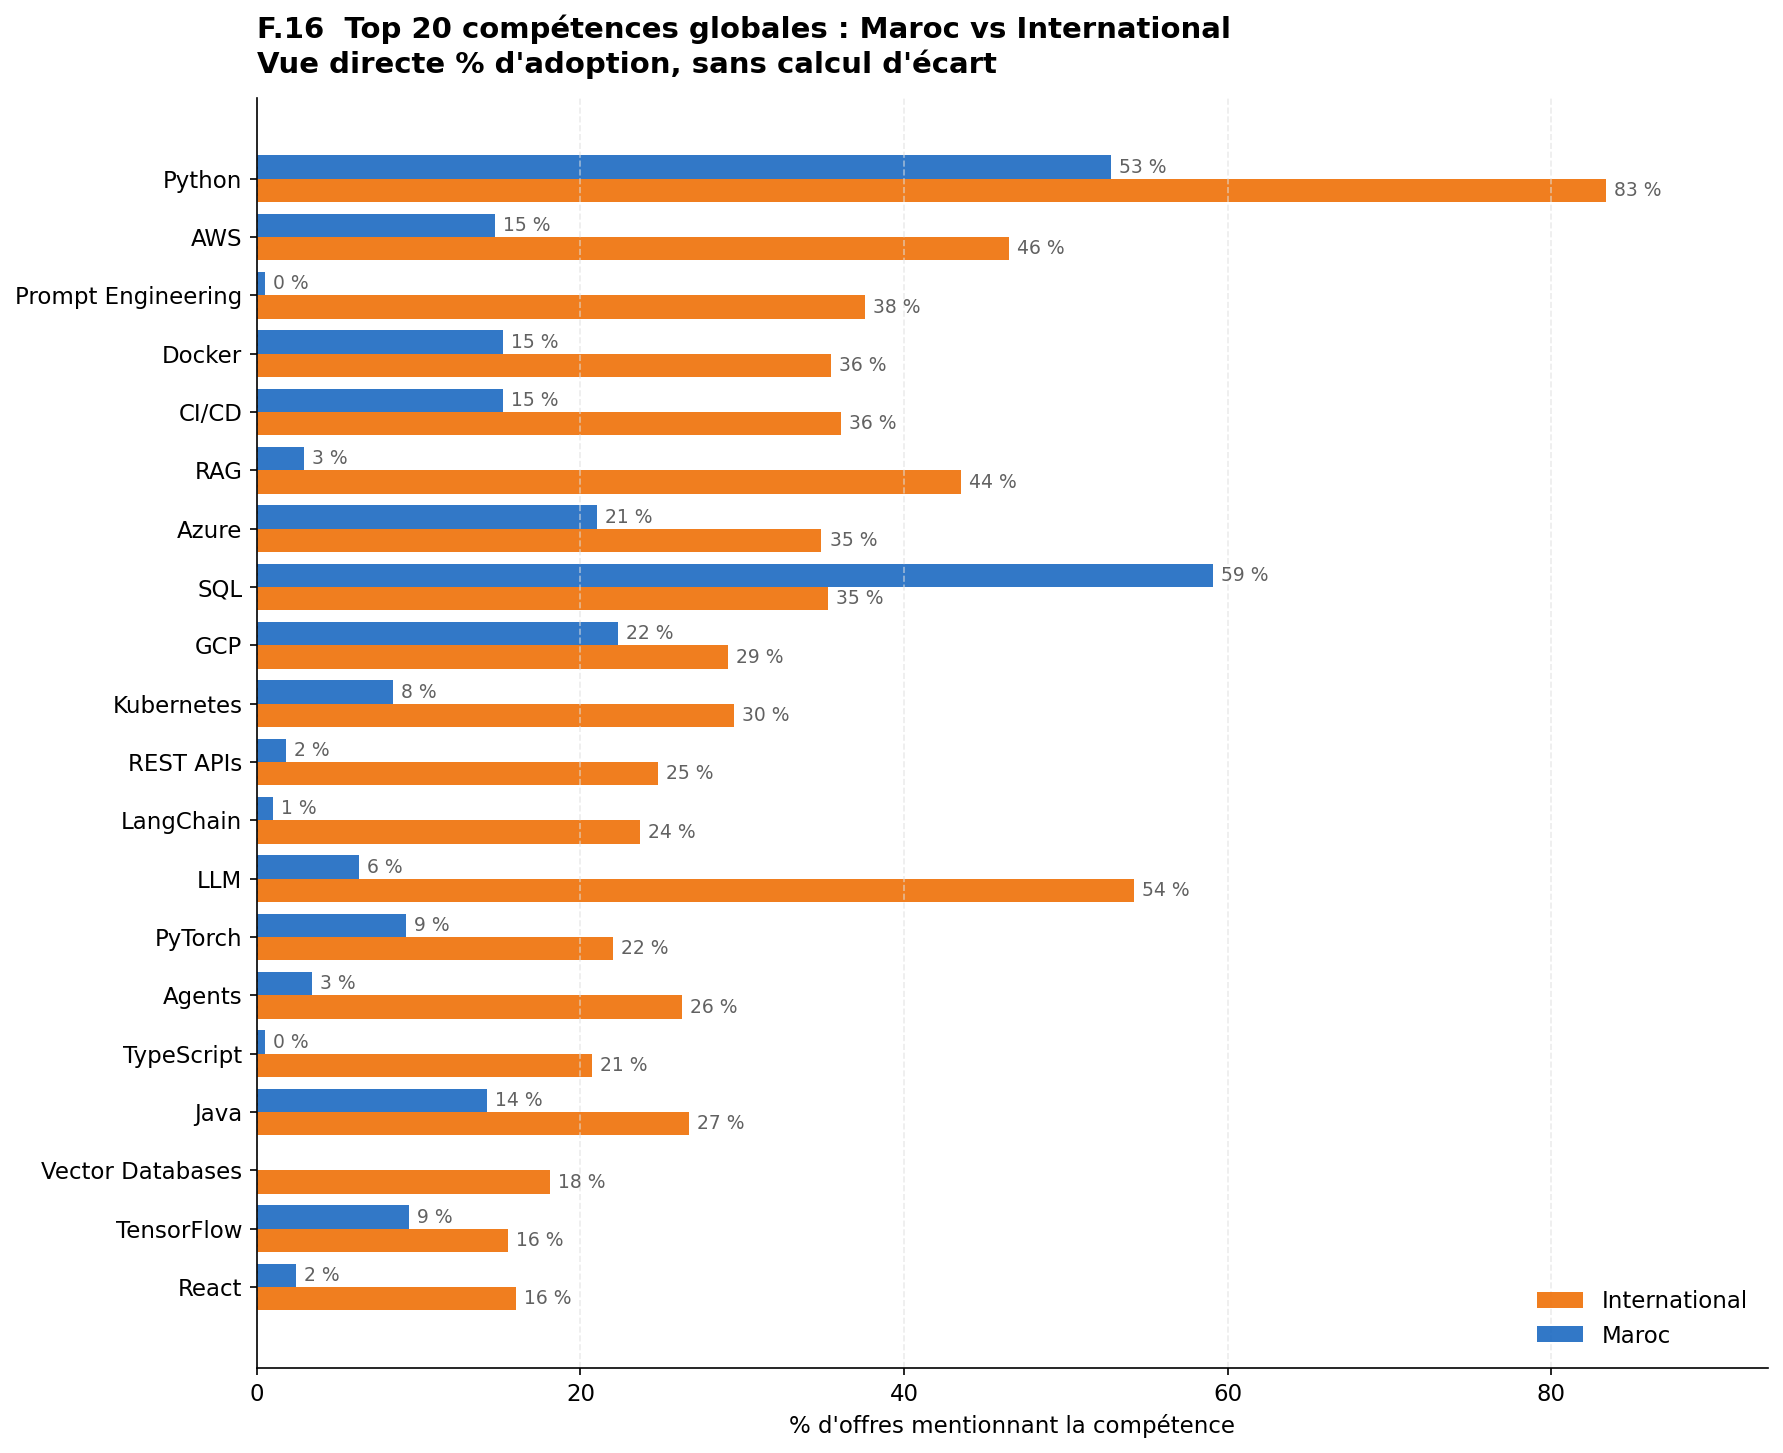
\includegraphics[width=0.88\textwidth]{f16_comparaison_top20_ma_vs_intl.png}
  \caption{Comparaison des vingt premi\`eres comp\'etences entre march\'e marocain et march\'e international.}
  \label{fig:f16-top20}
\end{figure}

Le premier groupe rassemble les comp\'etences universelles, pr\'esentes des deux c\^ot\'es \`a des fr\'equences \'elev\'ees, telles que Python (52,8\,\% au Maroc contre 83,4\,\% \`a l'international) ou SQL (59,1\,\% contre 35,3\,\%). Le second groupe rassemble les comp\'etences caract\'eristiques de l'Intelligence Artificielle g\'en\'erative, fortement pr\'esentes \`a l'international et marginales au Maroc (Large Language Model, RAG, Prompt Engineering, LangChain, Agents, Vector Databases). Le troisi\`eme groupe rassemble les comp\'etences sp\'ecifiques au Data Engineering classique, l\'eg\`erement plus repr\'esent\'ees au Maroc et stables \`a l'international (Spark, Airflow, Snowflake).

\section{Synth\`ese du portrait du march\'e observ\'e}

Les douze analyses descriptives pr\'esent\'ees dans ce chapitre convergent vers un portrait nuanc\'e du march\'e des comp\'etences en Intelligence Artificielle et Data Science observ\'e entre 2022 et 2026.

\`A l'international, et au regard du corpus de 3\,086 offres collect\'ees sur six pays via \texttt{builtin.com}, le march\'e est domin\'e par des profils AI-First (73,1\,\%), construit autour d'un \'ecosyst\`eme mature d'Intelligence Artificielle g\'en\'erative (Large Language Model, RAG, agents, LangChain, vector databases), structur\'e par des pratiques d'industrialisation cloud (AWS, Docker, Kubernetes, CI/CD) et orient\'e quasi exclusivement vers la production (97,0\,\%). Cette configuration traduit l'ach\`evement, au moins partiel, de la bascule vers l'Intelligence Artificielle g\'en\'erative d\'eclench\'ee par la sortie de ChatGPT en novembre 2022.

Au Maroc, et au regard des 381 offres collect\'ees sur 27 mois et six sources, le march\'e pr\'esente une physionomie sensiblement diff\'erente. Les profils Data Analytics (54,1\,\%) et Machine Learning traditionnel (33,9\,\%) y dominent, tandis que les profils AI-First restent minoritaires (12,1\,\%) et les profils AI-Support inexistants. La stack technique observ\'ee est centr\'ee sur SQL, Python, Power BI et les outils de Data Engineering classiques, et la p\'en\'etration des frameworks d'Intelligence Artificielle g\'en\'erative est marginale (LangChain \`a 1,0\,\%, RAG \`a 2,9\,\%, Large Language Model \`a 6,0\,\%).

Ces deux portraits ne doivent pas \^etre lus comme l'expression d'un retard absolu, dans la mesure o\`u la diff\'erence de volum\'etrie et la sp\'ecialisation tech industrielle de la source internationale constituent des biais discut\'es en section~5.2. Ils dessinent n\'eanmoins un d\'ecalage empiriquement mesurable, dont l'ampleur (\'ecart de 47,9 points sur Large Language Model, 40,6 points sur RAG, 37,1 points sur Prompt Engineering) suffit \`a motiver les analyses de structure et d'\'evolution conduites dans les chapitres suivants.

% =============== CHAPITRE 4 =================================
\chapter{\'Etudes comparatives et choix justifi\'es}

Le pr\'esent chapitre constitue le c\oe ur scientifique du rapport. Il rapporte les r\'esultats des trois \'etudes comparatives algorithmiques men\'ees dans le cadre du projet \skillnav, conform\'ement \`a l'exigence du sujet impos\'e pour le module M242 selon laquelle chaque t\^ache du pipeline doit faire l'objet d'une comparaison entre au moins trois algorithmes distincts. Les trois \'etudes correspondent respectivement aux axes Content Mining (reconnaissance d'entit\'es nomm\'ees), Structure Mining (d\'etection de communaut\'es) et Usage Mining (forecasting de s\'eries temporelles), et chacune se conclut par un choix d'algorithme retenu pour la version V1 du projet.

\section{Protocole exp\'erimental commun}

Les trois \'etudes partagent un ensemble de principes m\'ethodologiques destin\'es \`a garantir la reproductibilit\'e et la comparabilit\'e des r\'esultats. Les versions des biblioth\`eques Python utilis\'ees sont \'epingl\'ees dans le fichier \texttt{poetry.lock} \`a la racine du projet, ce qui assure qu'une ex\'ecution future du pipeline aboutira \`a des chiffres identiques. Les graines al\'eatoires des algorithmes non d\'eterministes sont fix\'ees explicitement (\texttt{seed=42} pour Label Propagation, \texttt{random\_state=42} pour la s\'election du gold set NER). Les ex\'ecutions multiples sont syst\'ematiquement utilis\'ees lorsqu'un algorithme pr\'esente une variance d'ex\'ecution non n\'egligeable, comme c'est le cas de Label Propagation dont la stabilit\'e est mesur\'ee sur cinq ex\'ecutions avec des graines diff\'erentes. Les m\'etriques utilis\'ees sont s\'electionn\'ees en fonction des sp\'ecificit\'es de chaque t\^ache : score F1 macro pour le NER, modularit\'e Q de Newman (2006) pour les communaut\'es, racine carr\'ee de l'erreur quadratique moyenne (RMSE) pour le forecasting.

\section{Reconnaissance d'entit\'es nomm\'ees : \'etude \S N2.1}

\subsection{Mod\`eles compar\'es}

Trois mod\`eles transformer ont \'et\'e retenus pour la comparaison, chacun repr\'esentant une option strat\'egique distincte. Le mod\`ele BERT multilingue (\texttt{Davlan/bert-base-multilingual-cased-ner-hrl}, 110 millions de param\`etres) repr\'esente l'option universelle, capable de traiter un corpus mixte fran\c{c}ais et anglais sans changement de mod\`ele. Le mod\`ele CamemBERT-NER (\texttt{Jean-Baptiste/camembert-ner}, 110 millions de param\`etres) repr\'esente l'option optimis\'ee pour le march\'e marocain. Le mod\`ele DistilBERT-NER (\texttt{dslim/distilbert-NER}, 66 millions de param\`etres) repr\'esente l'option l\'eg\`ere et rapide pour le march\'e international, dont le corpus collect\'e est essentiellement anglophone. Les trois mod\`eles sont h\'eberg\'es sur Hugging Face Hub et accessibles sans authentification, avec des licences compatibles avec un usage acad\'emique.

\subsection{Protocole d'\'evaluation}

L'\'evaluation repose sur un gold set de 30 fiches s\'electionn\'ees de mani\`ere diversifi\'ee (8 fiches Maroc et 22 fiches International, couvrant les quatre types de poste AI-First, AI-Support, ML-First et Data Analytics). La strat\'egie d'annotation retenue est celle de la \emph{distant supervision} document\'ee par Hovy et al. (2014), qui consiste \`a utiliser comme r\'ef\'erence les comp\'etences extraites et canonicalis\'ees par le pipeline structur\'e \'etabli pendant la phase de collecte. Ce choix m\'ethodologique est impos\'e par la contrainte temporelle du projet : l'annotation manuelle de 30 fiches par un bin\^ome repr\'esenterait 6 \`a 10 heures de travail, incompatibles avec le calendrier des sprints. Les limites de cette strat\'egie (propagation des biais de canonicalisation, sur-\'evaluation possible du rappel par matching en sous-cha\^ine) sont reprises au chapitre~5.2.2. Le matching entre entit\'es pr\'edites et comp\'etences gold s'op\`ere par sous-cha\^ine en mode insensible \`a la casse, et les trois m\'etriques retenues sont la pr\'ecision, le rappel et le score F1.

\subsection{R\'esultats chiffr\'es}

Les r\'esultats obtenus sur le gold set sont synth\'etis\'es dans le tableau~\ref{tab:ner-results}.

\begin{table}[H]
  \centering
  \caption{\'Etude comparative \S N2.1 des trois mod\`eles NER \'evalu\'es sur le gold set de 30 fiches.}
  \label{tab:ner-results}
  \small
  \begin{tabular}{lrrrrrrl}
    \toprule
    \rowcolor{softblue}\textbf{Mod\`ele} & \textbf{Param.} & \textbf{Pr\'ec.} & \textbf{Rappel} & \textbf{F1} & \textbf{Tps (s)} & \textbf{Ent.} & \textbf{Skills gold} \\
    \midrule
    BERT multilingue & 110\,M & 0,308 & 0,029 & 0,054 & 0,29 & 49 & 16/543 \\
    CamemBERT-NER & 110\,M & 0,454 & 0,282 & 0,348 & 0,38 & 310 & 153/543 \\
    \textbf{DistilBERT-NER} & 66\,M & 0,443 & \textbf{0,484} & \textbf{0,463} & \textbf{0,15} & 532 & 263/543 \\
    \bottomrule
  \end{tabular}
\end{table}

\begin{figure}[H]
  \centering
  \begin{subfigure}[t]{0.48\textwidth}
    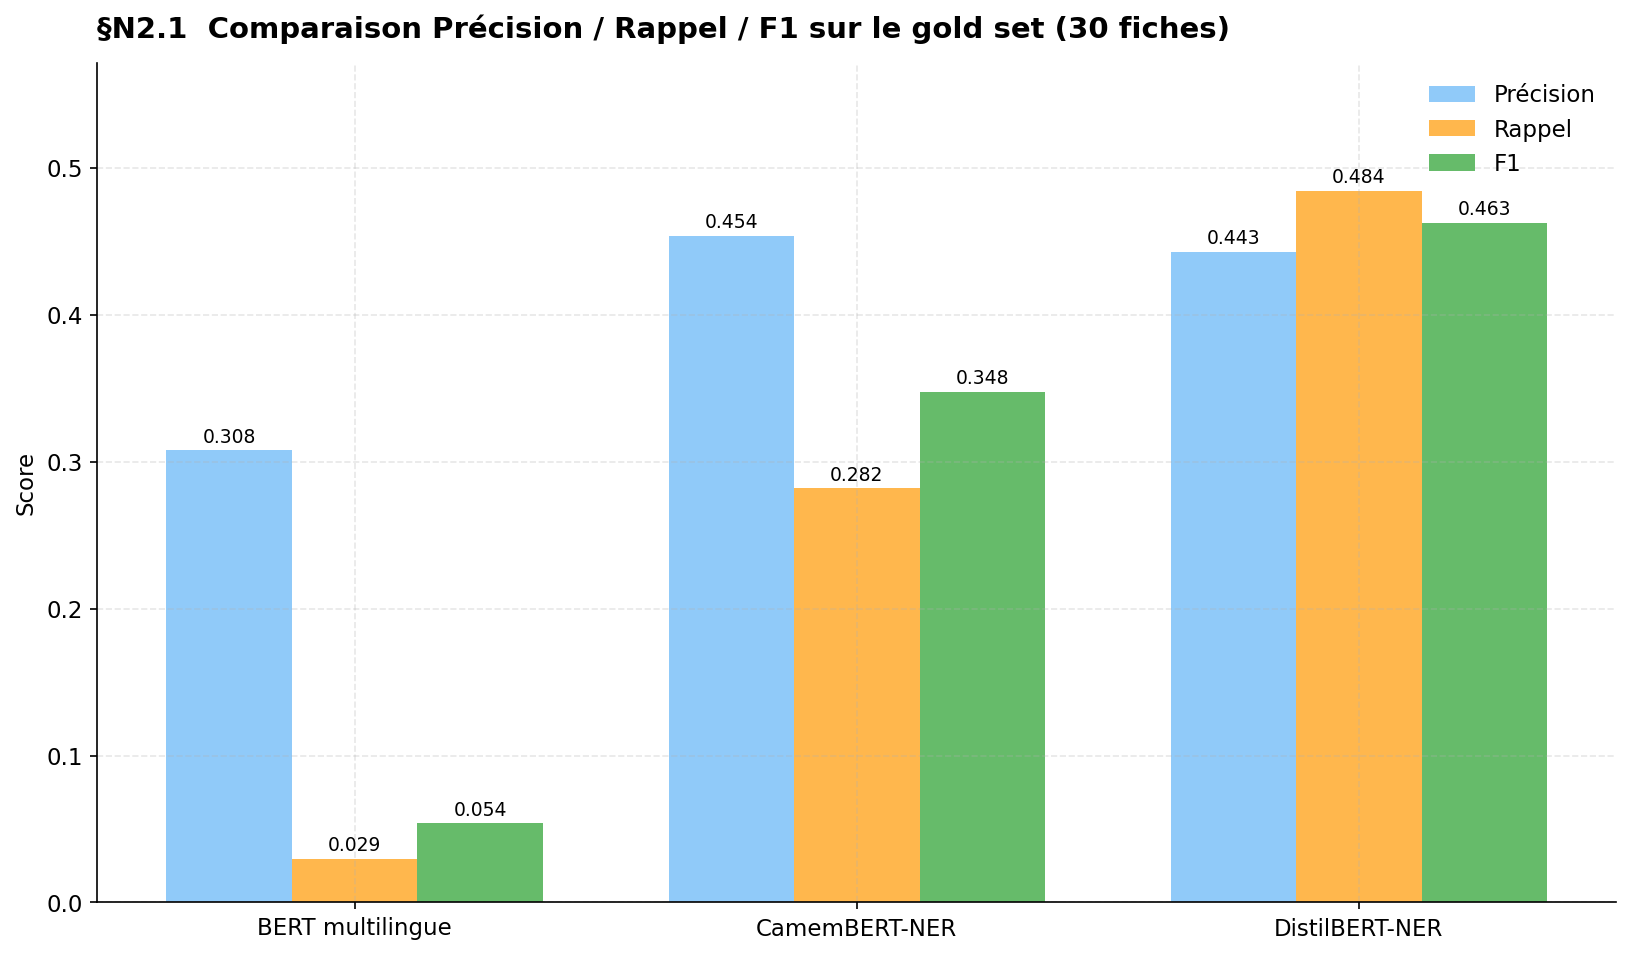
\includegraphics[width=\textwidth]{n21_comparaison_ner.png}
    \caption{Pr\'ecision, rappel et F1.}
  \end{subfigure}\hfill
  \begin{subfigure}[t]{0.48\textwidth}
    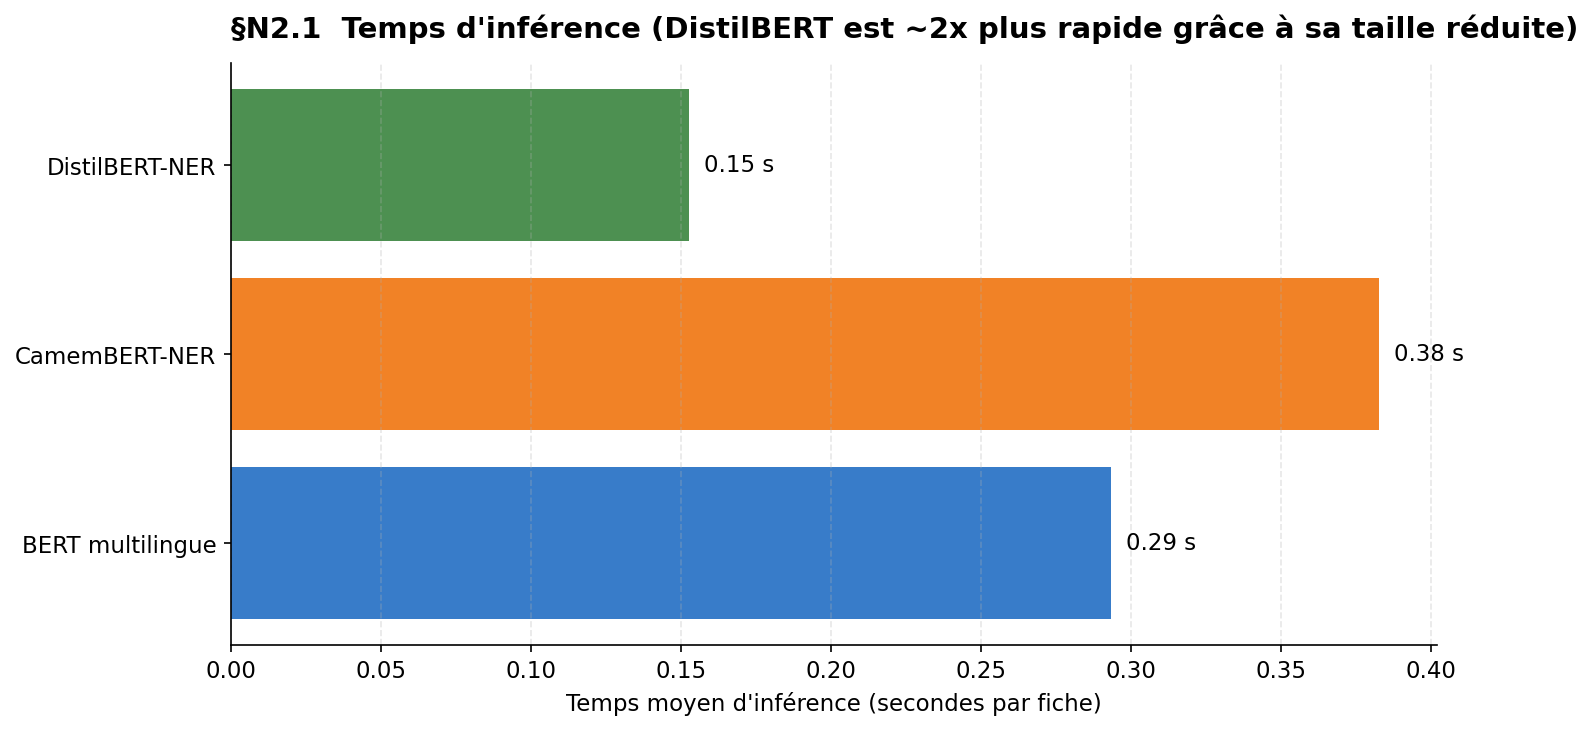
\includegraphics[width=\textwidth]{n21_temps_inference.png}
    \caption{Temps moyen d'inf\'erence (CPU).}
  \end{subfigure}
  \caption{Comparaison des trois mod\`eles NER : qualit\'e et performance.}
  \label{fig:ner-comp}
\end{figure}

\subsection{Discussion}

Trois enseignements ressortent de cette comparaison. D'abord, BERT multilingue est inexploitable : son rappel de 0,029 traduit une quasi-absence de d\'etection sur les textes techniques mixtes fran\c{c}ais-anglais du corpus, le mod\`ele ayant \'et\'e pr\'e-entra\^in\'e sur un corpus g\'en\'eraliste couvrant dix langues. Sa pr\'ecision honorable (0,308) ne compense pas l'identification de moins de deux entit\'es par fiche en moyenne. Ensuite, CamemBERT-NER affiche des r\'esultats \'equilibr\'es (pr\'ecision 0,454 ; rappel 0,282 ; F1 0,348), coh\'erents avec sa sp\'ecialisation fran\c{c}aise. Sa limite tient au corpus lui-m\^eme : 73\,\% des offres sont r\'edig\'ees en anglais, donc hors de son p\'erim\`etre d'entra\^inement. Enfin, DistilBERT-NER s'impose avec le meilleur F1 (0,463), port\'e par un rappel \'elev\'e (0,484). Le mod\`ele atteint ce r\'esultat avec 40\,\% de param\`etres en moins (66\,M contre 110\,M) et un temps d'inf\'erence divis\'e par deux (0,15 seconde par fiche).

\subsection{It\'eration zero-shot avec GLiNER}

Au-del\`a de la comparaison principale des trois mod\`eles transformer classiques, une it\'eration compl\'ementaire a \'et\'e men\'ee avec le mod\`ele GLiNER (Generalist Lightweight Named Entity Recognition) en mode zero-shot, c'est-\`a-dire sans \'etape de fine-tuning pr\'ealable. Cette it\'eration exploite la capacit\'e de GLiNER \`a recevoir une liste d'\'etiquettes cibles au moment de l'inf\'erence, ce qui permet d'orienter l'extraction vers les types d'entit\'es effectivement pr\'esents dans le corpus \skillnav (SKILL, TOOL, FRAMEWORK, MODEL, LANGUAGE, ROLE).

\begin{figure}[H]
  \centering
  \begin{subfigure}[t]{0.48\textwidth}
    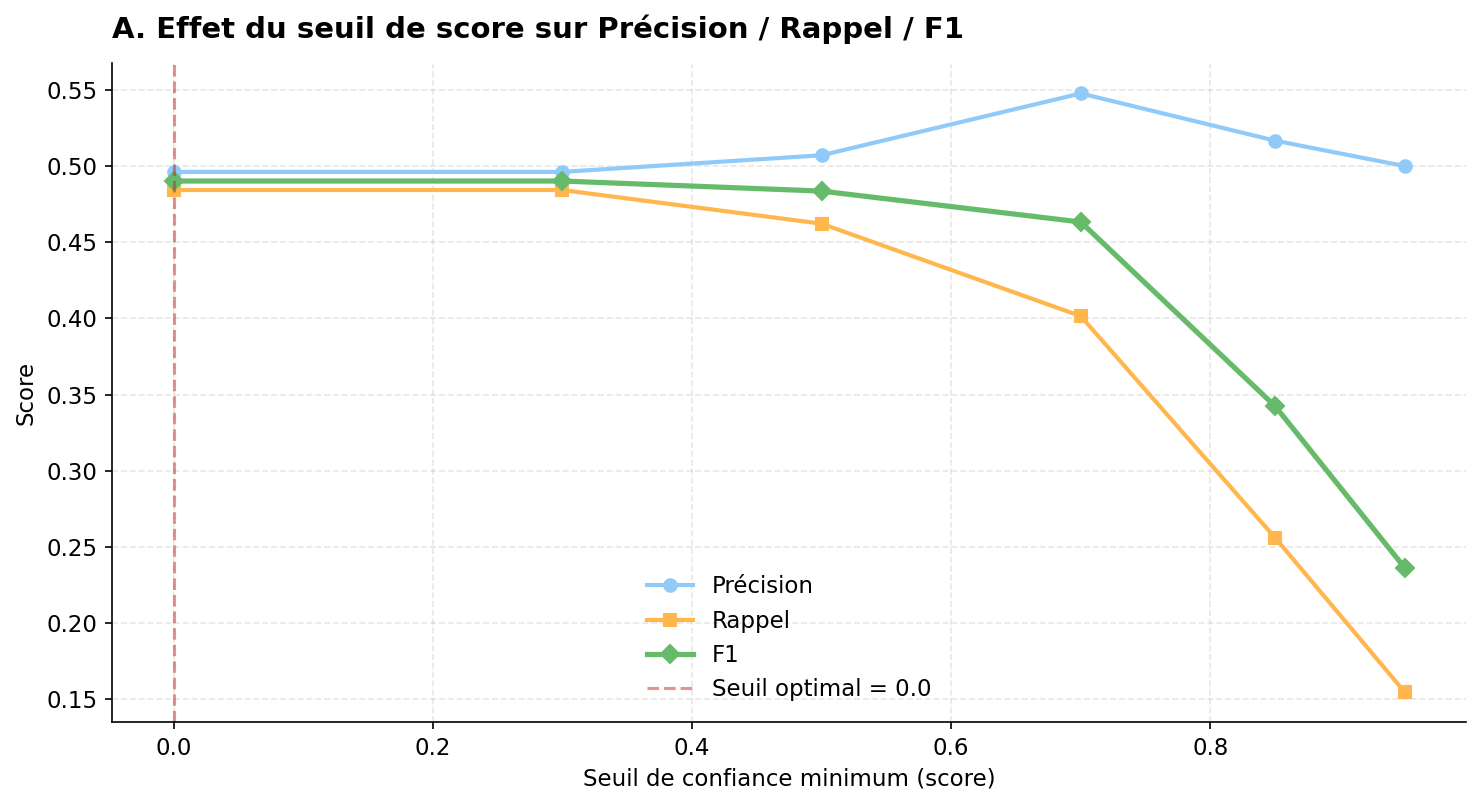
\includegraphics[width=\textwidth]{n21_amelioration_A_seuil.png}
    \caption{Effet du seuil d'abstention.}
  \end{subfigure}\hfill
  \begin{subfigure}[t]{0.48\textwidth}
    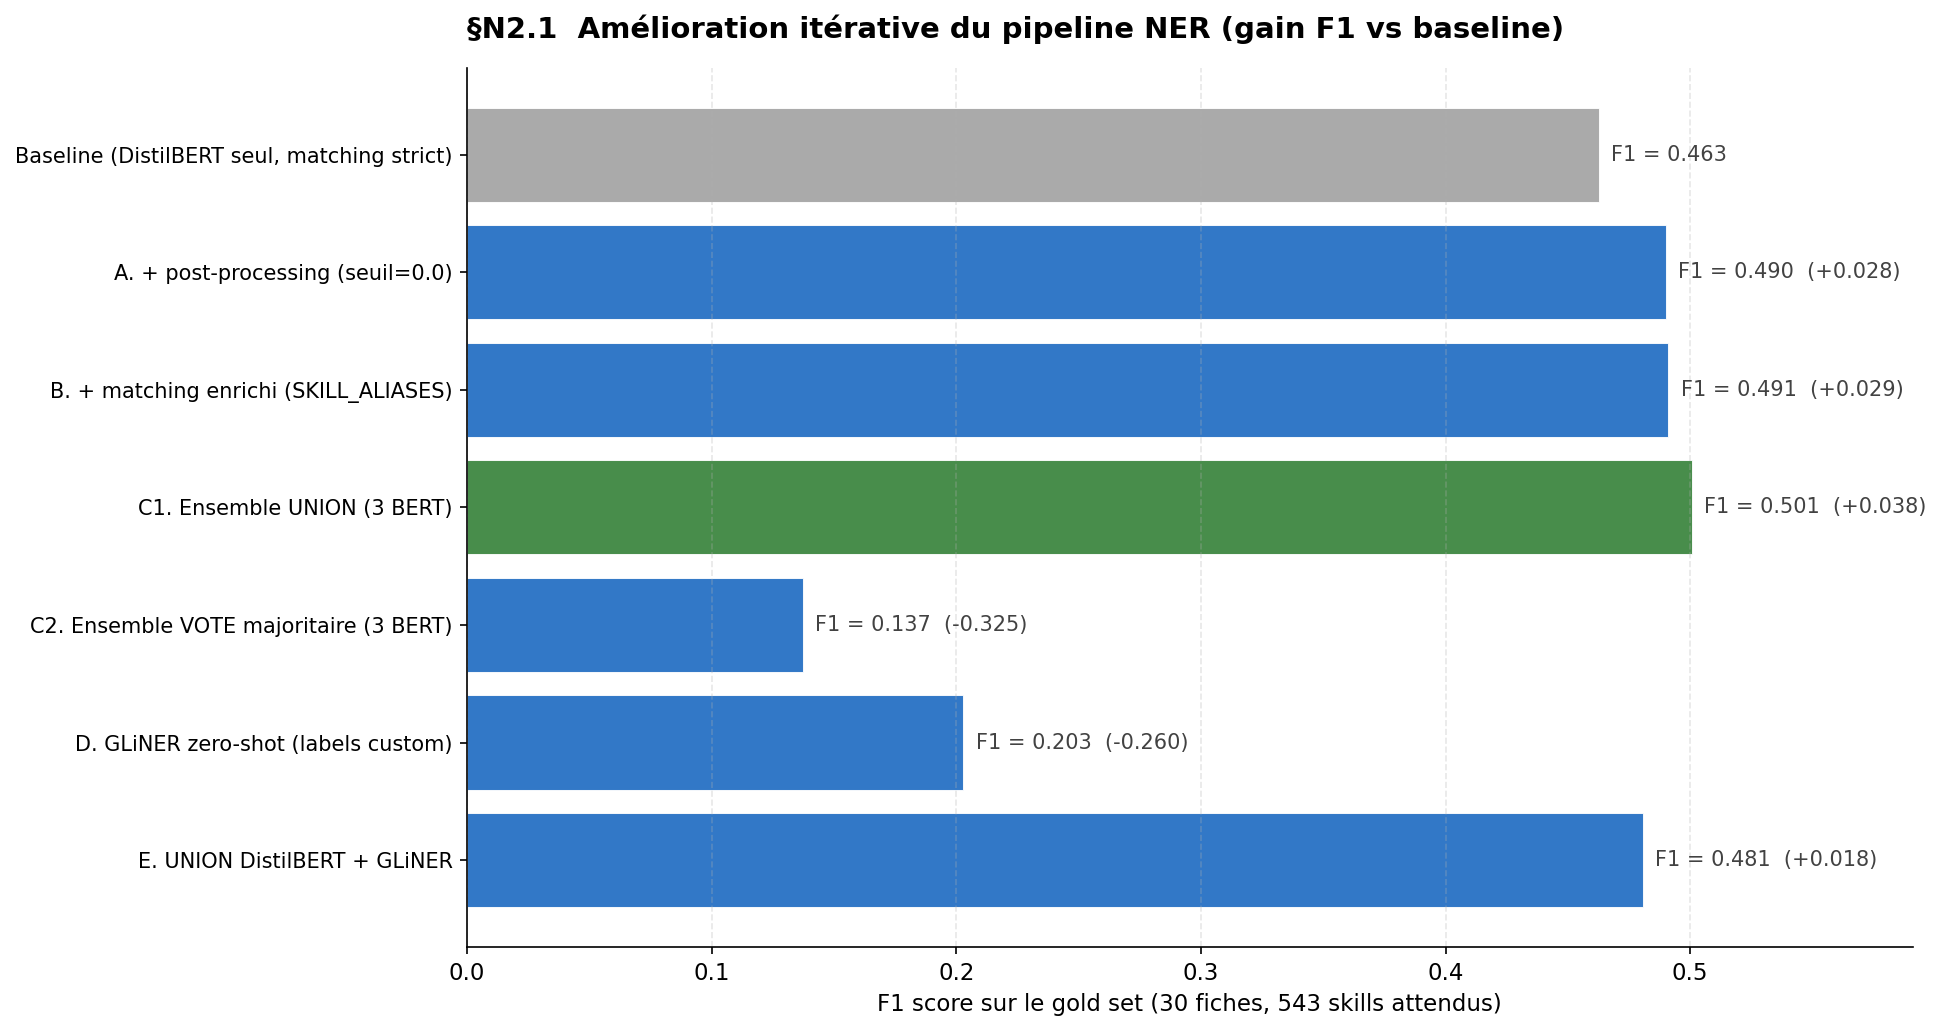
\includegraphics[width=\textwidth]{n21_amelioration_recap.png}
    \caption{R\'ecapitulatif comparatif.}
  \end{subfigure}
  \caption{It\'eration zero-shot GLiNER compar\'ee aux trois mod\`eles transformer classiques.}
  \label{fig:gliner}
\end{figure}

\subsection{Choix retenu et perspectives}

Le mod\`ele DistilBERT-NER est retenu pour le pipeline de production de la version V1 de \skillnav. Trois crit\`eres justifient ce choix. Le score F1 obtenu sur le gold set (0,463) est le plus \'elev\'e des trois mod\`eles compar\'es. Le temps d'inf\'erence par fiche (0,15 seconde) est le plus court, ce qui correspond \`a un temps total inf\'erieur \`a neuf minutes pour le traitement complet des 3\,467 fiches du corpus. L'empreinte m\'emoire est 40\,\% plus faible que celle des deux autres mod\`eles, ce qui rend le mod\`ele d\'eployable sur les services cloud gratuits envisag\'es pour le dashboard \skillnav.

Plusieurs pistes d'am\'elioration sont identifi\'ees et report\'ees au chapitre~5.4 comme perspectives V1.5 : le fine-tuning de DistilBERT sur un gold set \'etendu \`a 100 ou 200 fiches annot\'ees manuellement (gain F1 attendu entre 0,15 et 0,25 selon Lample et al., 2016), la mise en place d'un ensemble combinant DistilBERT (rappel) et CamemBERT (pr\'ecision sur les fiches en fran\c{c}ais), et l'\'evaluation de mod\`eles plus r\'ecents tels que \texttt{mDeBERTa-NER} ou la version fine-tun\'ee de GLiNER.

\section{D\'etection de communaut\'es dans le graphe de comp\'etences : \'etude \S N2.2}

\subsection{Protocole exp\'erimental}

L'\'etude porte sur le graphe Skill vers Skill construit par projection de co-occurrence \`a partir des 3\,467 offres du corpus, dont la m\'ethodologie est expos\'ee en section~2.4. Le graphe comporte 3\,937 n\oe uds repr\'esentant les comp\'etences canoniques, et 10\,324 ar\^etes pond\'er\'ees par le nombre d'offres dans lesquelles les deux comp\'etences co-occurrent. Le seuil minimum de co-occurrence est fix\'e \`a 2, ce qui \'ecarte les paires fortuites observ\'ees dans une seule offre. Trois caract\'eristiques importantes du graphe sont \`a noter avant la lecture des r\'esultats. Sa densit\'e est tr\`es faible (0,0013), ce qui est attendu sur un graphe technique de cette taille. Le graphe comporte 2\,768 composantes connexes, ce qui signifie que la majorit\'e des n\oe uds sont des ilots isol\'es correspondant \`a des comp\'etences rares ou tr\`es sp\'ecialis\'ees qui ne co-occurrent qu'avec une ou deux autres comp\'etences sans pont vers le graphe principal. Le degr\'e moyen est de 5,24, mais cette moyenne masque une distribution tr\`es in\'egale dans laquelle les comp\'etences universelles (Python, SQL) sont connect\'ees \`a plus de deux cents autres comp\'etences alors que les comp\'etences sp\'ecialis\'ees ne le sont qu'\`a quelques-unes.

Trois algorithmes de d\'etection de communaut\'es sont compar\'es sur ce graphe : Louvain (Blondel et al., 2008) dans son impl\'ementation \texttt{python-louvain}, Leiden (Traag et al., 2019) dans son impl\'ementation \texttt{igraph}, et Label Propagation (Raghavan et al., 2007) dans son impl\'ementation \texttt{networkx}. La m\'etrique de qualit\'e retenue est la modularit\'e Q d\'efinie par Newman (2006), dont la valeur s'\'etale entre $-1$ et 1 et qui mesure la densit\'e des ar\^etes intra-communaut\'es relativement \`a un graphe al\'eatoire de m\^eme distribution de degr\'es.

\subsection{R\'esultats chiffr\'es}

\begin{table}[H]
  \centering
  \caption{\'Etude comparative \S N2.2 des trois algorithmes de d\'etection de communaut\'es sur le graphe Skill vers Skill.}
  \label{tab:communautes}
  \small
  \begin{tabularx}{\textwidth}{l r r r L{4.5cm}}
    \toprule
    \rowcolor{softblue}\textbf{Algorithme} & \textbf{Mod. Q} & \textbf{Nb communaut\'es} & \textbf{Tps (s)} & \textbf{Notes} \\
    \midrule
    Louvain & 0,2943 & 2\,782 & 1,101 & M\'ethode it\'erative classique \\
    \textbf{Leiden} & \textbf{0,2988} & 2\,784 & 0,383 & Connexit\'e garantie, modularit\'e maximale \\
    Label Propagation & 0,1476 & 2\,784 & 0,498 & Rapide mais fragmentation forte \\
    \bottomrule
  \end{tabularx}
\end{table}

\begin{figure}[H]
  \centering
  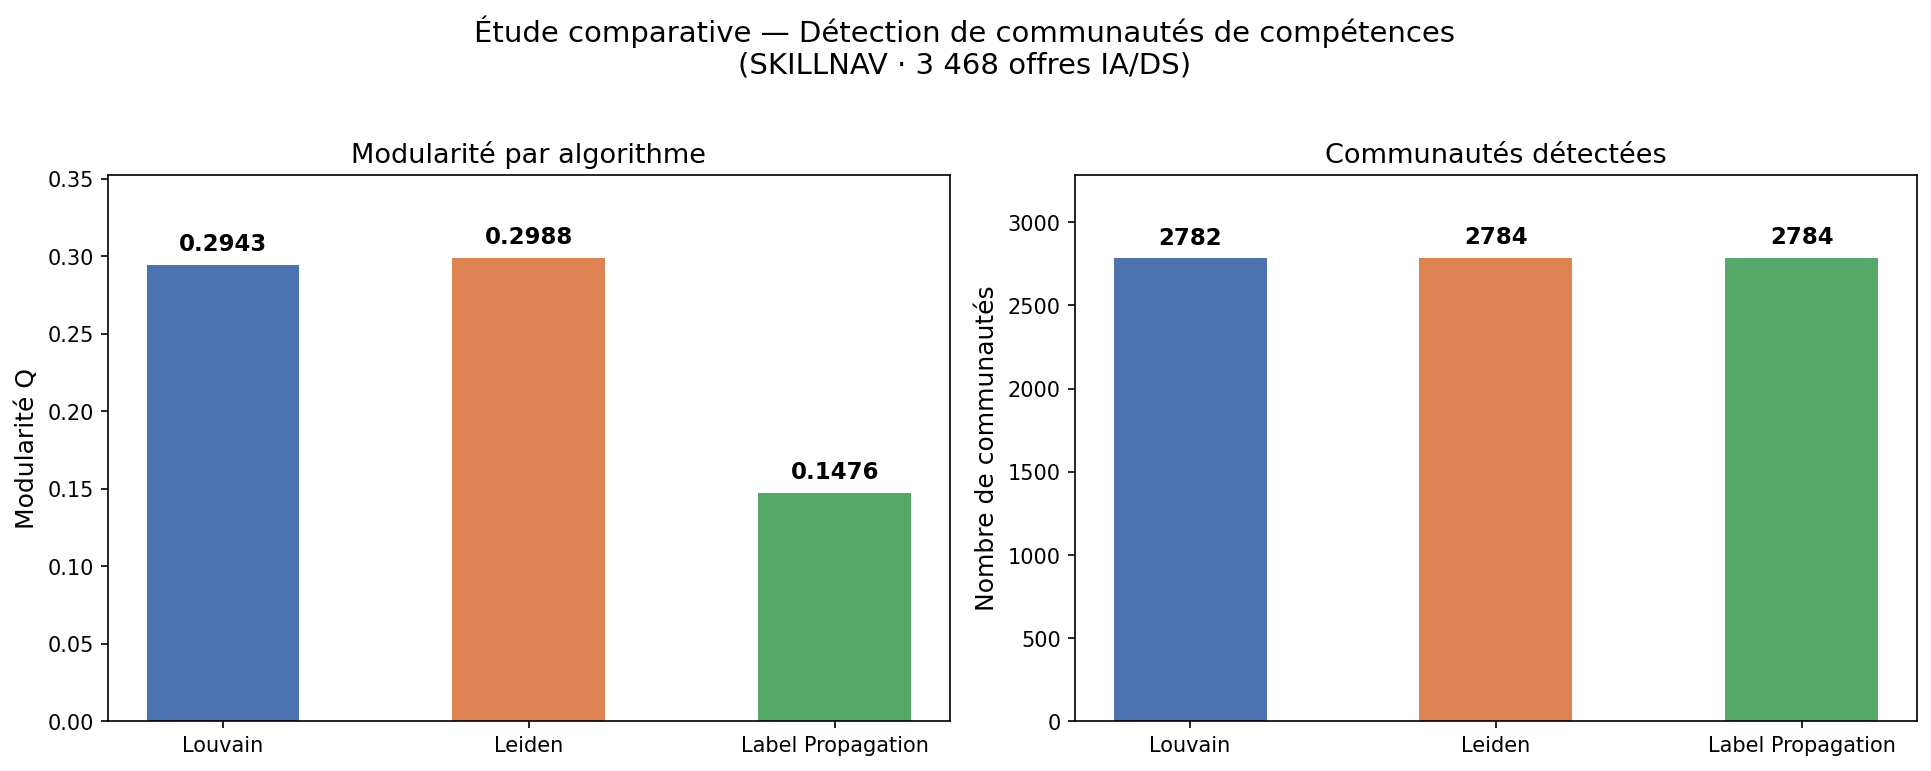
\includegraphics[width=0.78\textwidth]{community_comparison.png}
  \caption{Comparaison des trois algorithmes de d\'etection de communaut\'es : modularit\'e et nombre de communaut\'es d\'etect\'ees.}
  \label{fig:comm-comp}
\end{figure}

Le nombre \'elev\'e de communaut\'es (entre 2\,782 et 2\,784 selon l'algorithme) s'explique directement par la pr\'esence des 2\,768 composantes connexes du graphe : chaque composante isol\'ee constitue par construction sa propre communaut\'e triviale. La structure communautaire pertinente, c'est-\`a-dire celle qui apporte une information s\'emantique exploitable, se concentre dans le sous-graphe principal connect\'e, dont l'analyse qualitative est conduite en section~4.3.5.

\subsection{Stabilit\'e de l'algorithme Label Propagation}

L'algorithme Label Propagation est par construction non d\'eterministe. Sa stabilit\'e est mesur\'ee en ex\'ecutant cinq fois l'algorithme avec cinq graines diff\'erentes.

\begin{table}[H]
  \centering
  \caption{Stabilit\'e de Label Propagation sur cinq ex\'ecutions avec graines al\'eatoires diff\'erentes.}
  \label{tab:label-prop-stab}
  \begin{tabular}{rrr}
    \toprule
    \rowcolor{softblue}\textbf{Graine} & \textbf{Modularit\'e Q} & \textbf{Nb communaut\'es} \\
    \midrule
    0 & 0,1486 & 2\,786 \\
    1 & 0,1486 & 2\,784 \\
    2 & 0,1494 & 2\,785 \\
    3 & 0,1484 & 2\,785 \\
    4 & 0,1485 & 2\,785 \\
    \midrule
    \multicolumn{1}{l}{\textit{Moyenne}} & 0,1487 & 2\,785 \\
    \multicolumn{1}{l}{\textit{\'Ecart-type}} & 0,0004 & 0,89 \\
    \bottomrule
  \end{tabular}
\end{table}

La variance observ\'ee est tr\`es faible. Cette stabilit\'e empirique inattendue s'explique par la structure particuli\`ere du graphe \skillnav, domin\'ee par des composantes isol\'ees. Les algorithmes Louvain et Leiden sont d\'eterministes par construction, avec un \'ecart-type strictement nul.

\subsection{Centralit\'e des comp\'etences par PageRank}

Au-del\`a de la partition en communaut\'es, l'analyse de la centralit\'e de chaque comp\'etence par l'algorithme PageRank (Page et al., 1999), ex\'ecut\'e avec un facteur d'amortissement \texttt{alpha=0.85}, fournit un classement des comp\'etences les plus structurantes du march\'e. Le top 20 des comp\'etences pivot est reproduit dans la figure~\ref{fig:pagerank} et synth\'etis\'e dans le tableau~\ref{tab:pagerank-top10}.

\begin{figure}[H]
  \centering
  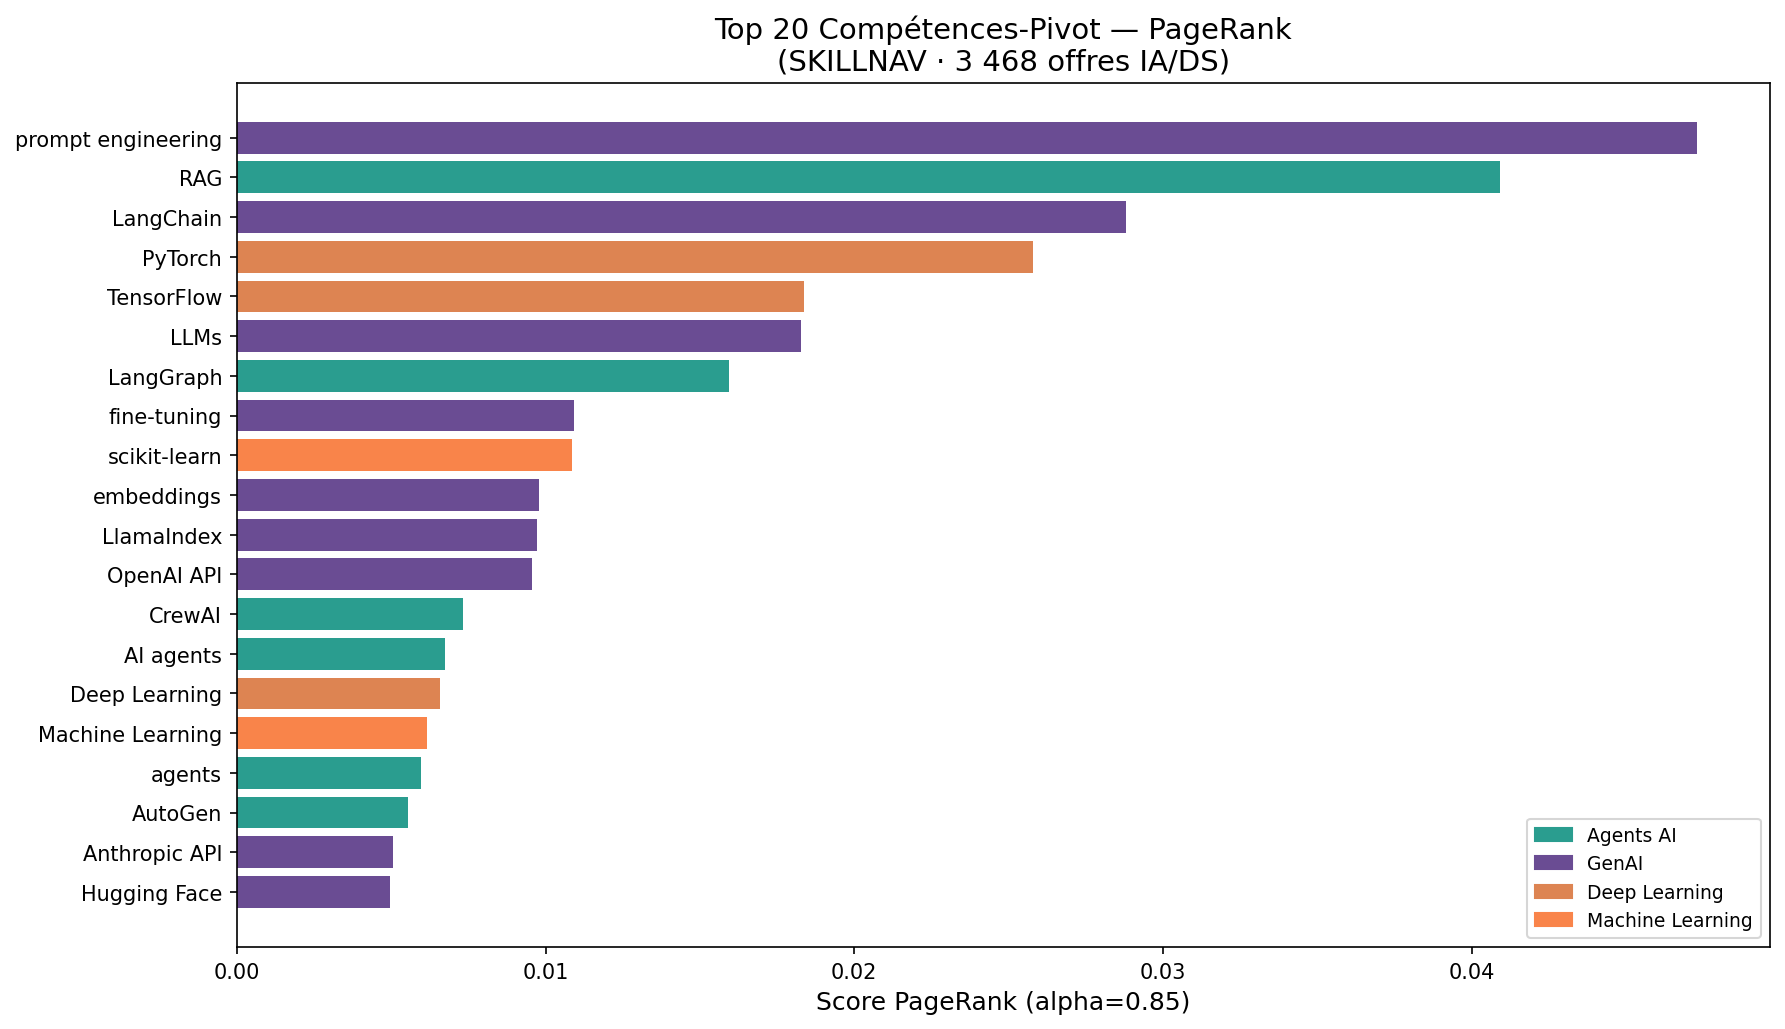
\includegraphics[width=0.82\textwidth]{pagerank_top20.png}
  \caption{Top 20 des comp\'etences les plus centrales selon le PageRank.}
  \label{fig:pagerank}
\end{figure}

\begin{table}[H]
  \centering
  \caption{Top 10 des comp\'etences les plus centrales selon le PageRank.}
  \label{tab:pagerank-top10}
  \begin{tabular}{rlrl}
    \toprule
    \rowcolor{softblue}\textbf{Rang} & \textbf{Comp\'etence} & \textbf{Score} & \textbf{Famille} \\
    \midrule
    1 & prompt engineering & 0,0473 & GenAI \\
    2 & RAG & 0,0409 & Agents AI \\
    3 & LangChain & 0,0288 & GenAI \\
    4 & PyTorch & 0,0258 & Deep Learning \\
    5 & TensorFlow & 0,0184 & Deep Learning \\
    6 & LLMs & 0,0183 & GenAI \\
    7 & LangGraph & 0,0159 & Agents AI \\
    8 & fine-tuning & 0,0109 & GenAI \\
    9 & scikit-learn & 0,0109 & Machine Learning \\
    10 & embeddings & 0,0098 & GenAI \\
    \bottomrule
  \end{tabular}
\end{table}

Sept des dix premi\`eres comp\'etences pivot appartiennent \`a l'\'ecosyst\`eme de l'Intelligence Artificielle g\'en\'erative ou des agents conversationnels. Le constat empirique est sans ambigu\"it\'e : \`a l'horizon mai 2026, les comp\'etences structurantes du march\'e des emplois en Intelligence Artificielle sont massivement issues de la vague Generative AI d\'eclench\'ee par la sortie publique de ChatGPT en novembre 2022. Les comp\'etences classiques du Machine Learning (PyTorch, TensorFlow, scikit-learn) restent pr\'esentes dans le top 10 mais c\`edent leur position de t\^ete aux comp\'etences g\'en\'eratives.

\subsection{Analyse qualitative des cinq plus grandes communaut\'es Louvain}

L'inspection des cinq plus grandes communaut\'es d\'etect\'ees par Louvain dans le sous-graphe principal connect\'e r\'ev\`ele une structuration s\'emantique coh\'erente. La premi\`ere communaut\'e, comportant 542 comp\'etences, est centr\'ee sur l'Intelligence Artificielle g\'en\'erative et les agents conversationnels, avec en t\^ete prompt engineering, RAG, LangChain, LLMs et LangGraph. La deuxi\`eme communaut\'e, comportant 291 comp\'etences, regroupe les comp\'etences classiques du Deep Learning autour de PyTorch, TensorFlow, scikit-learn et Keras. La troisi\`eme communaut\'e, comportant 146 comp\'etences, est inattendue et regroupe les environnements de d\'eveloppement assist\'es par Intelligence Artificielle g\'en\'erative (Cursor, GitHub Copilot, Claude Code, Gemini, n8n) ainsi que les outils d'orchestration SaaS du quotidien (Salesforce, Jira, ServiceNow). La quatri\`eme communaut\'e, comportant 83 comp\'etences, regroupe les comp\'etences classiques du Data Analytics et de l'analyse de donn\'ees (Machine Learning, Python, SQL, GCP, Power BI, R, Statistics, Azure, Spark, Tableau), correspondant \`a la stack typique du march\'e marocain identifi\'ee en section~3.5.1. La cinqui\`eme communaut\'e, comportant 23 comp\'etences, regroupe les mod\`eles propri\'etaires (Llama, Mistral, GPT-4) avec les cadres de conformit\'e r\'eglementaire (GDPR, HIPAA, CCPA, SOX, MITRE ATT\&CK), traduisant l'attention croissante port\'ee \`a la conformit\'e dans le d\'eploiement industriel des mod\`eles de langage.

\subsection{Choix retenu et perspectives}

L'algorithme Leiden est retenu comme m\'ethode de r\'ef\'erence pour la version V1 de \skillnav. Trois crit\`eres justifient ce choix. La modularit\'e Q obtenue (0,2988) est la plus \'elev\'ee des trois algorithmes compar\'es. La connexit\'e interne des communaut\'es est garantie par construction (Traag et al., 2019), contrairement \`a Louvain qui peut produire des communaut\'es mal connect\'ees dans des cas particuliers. Le temps d'ex\'ecution (0,383 seconde) est le plus court des trois. Louvain est n\'eanmoins conserv\'e comme r\'ef\'erence narrative dans le rapport et le dashboard, dans la mesure o\`u il s'agit de l'algorithme historiquement le plus cit\'e dans la litt\'erature. Label Propagation est document\'e comme baseline rapide mais inadapt\'e \`a la qualit\'e de partitionnement attendue.

\section{Forecasting des s\'eries temporelles de comp\'etences : \'etude \S N2.3}

\subsection{Protocole exp\'erimental}

L'\'etude porte sur la pr\'evision de l'\'evolution hebdomadaire des dix comp\'etences les plus fr\'equentes du corpus sur la fen\^etre temporelle dense de janvier \`a mai 2026. La m\'ethodologie de construction des s\'eries temporelles est expos\'ee en section~2.5. Pour chaque comp\'etence du top 10, la s\'erie hebdomadaire est obtenue par agr\'egation ISO week des dates de publication des offres, avec remplissage par z\'ero pour les semaines sans occurrence. Les trois derni\`eres semaines (du 27 avril au 17 mai 2026) sont tronqu\'ees du fait de l'artefact de collecte expos\'e en section~2.5.2, ce qui laisse une s\'erie effective de seize semaines exploitable pour le forecasting.

Trois mod\`eles de forecasting issus de familles distinctes sont compar\'es : ARIMA (Box et Jenkins, 1976) dans son impl\'ementation \texttt{statsmodels} avec s\'election automatique des param\`etres par minimisation du crit\`ere d'Akaike, Prophet (Taylor et Letham, 2018) dans son impl\'ementation \texttt{prophet}, et LSTM (Hochreiter et Schmidhuber, 1997) dans son impl\'ementation \texttt{neuralforecast}. Le partitionnement train et test est fix\'e \`a quinze semaines d'entra\^inement et quatre semaines de test, avec un horizon de pr\'ediction suppl\'ementaire de quatre semaines. La m\'etrique principale de s\'election est RMSE.

\subsection{R\'esultats agr\'eg\'es}

\begin{table}[H]
  \centering
  \caption{\'Etude comparative \S N2.3 des trois mod\`eles de forecasting sur le top 10 des comp\'etences.}
  \label{tab:forecast-agg}
  \begin{tabular}{lrrl}
    \toprule
    \rowcolor{softblue}\textbf{Mod\`ele} & \textbf{RMSE m\'edian} & \textbf{Victoires sur 10} & \textbf{Famille} \\
    \midrule
    \textbf{ARIMA} & \textbf{17,21} & \textbf{5} & Statistique classique \\
    Prophet & 17,96 & 3 & D\'ecomposition (Meta) \\
    LSTM & 21,51 & 2 & Deep learning \\
    \bottomrule
  \end{tabular}
\end{table}

\begin{figure}[H]
  \centering
  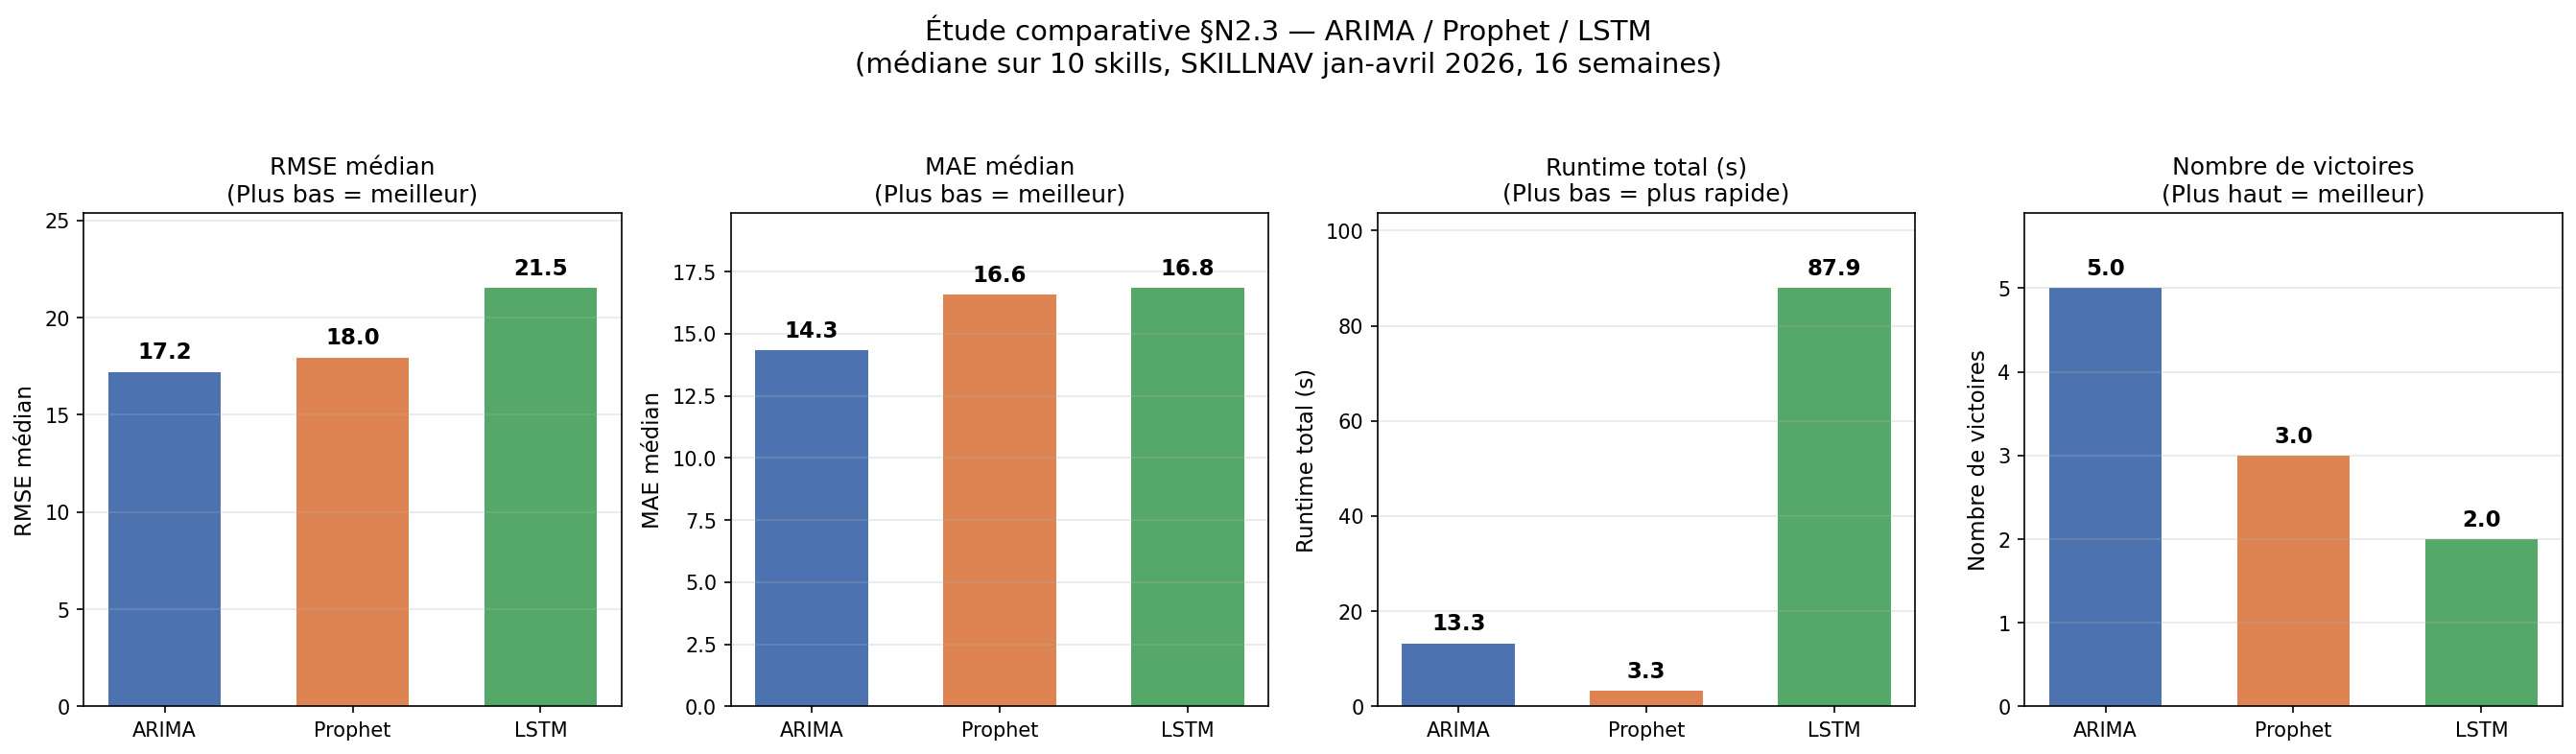
\includegraphics[width=0.78\textwidth]{forecast_comparison.png}
  \caption{Comparaison agr\'eg\'ee des trois mod\`eles de forecasting (RMSE m\'edian et nombre de victoires).}
  \label{fig:forecast-comp}
\end{figure}

\subsection{D\'etail des r\'esultats par comp\'etence}

\begin{table}[H]
  \centering
  \caption{D\'etail par comp\'etence des RMSE obtenues par chacun des trois mod\`eles.}
  \label{tab:forecast-detail}
  \small
  \begin{tabular}{lrrrrl}
    \toprule
    \rowcolor{softblue}\textbf{Comp\'etence} & \textbf{Famille} & \textbf{ARIMA} & \textbf{Prophet} & \textbf{LSTM} & \textbf{Gagnant} \\
    \midrule
    Prompt engineering & GenAI & 17,24 & 17,60 & 40,39 & ARIMA \\
    RAG & Agents AI & 21,85 & 22,65 & 31,39 & ARIMA \\
    LangChain & GenAI & 19,98 & 30,18 & 20,10 & ARIMA \\
    PyTorch & Deep Learning & 17,18 & 23,14 & 24,28 & ARIMA \\
    LLMs & GenAI & 23,77 & 18,31 & 22,92 & Prophet \\
    TensorFlow & Deep Learning & 22,52 & 22,25 & 31,43 & Prophet \\
    LangGraph & Agents AI & 7,00 & 17,27 & 6,94 & LSTM \\
    Fine-tuning & GenAI & 10,30 & 5,45 & 7,53 & Prophet \\
    OpenAI API & GenAI & 13,64 & 9,12 & 7,31 & LSTM \\
    embeddings & GenAI & 8,71 & 9,25 & 9,88 & ARIMA \\
    \bottomrule
  \end{tabular}
\end{table}

\begin{figure}[H]
  \centering
  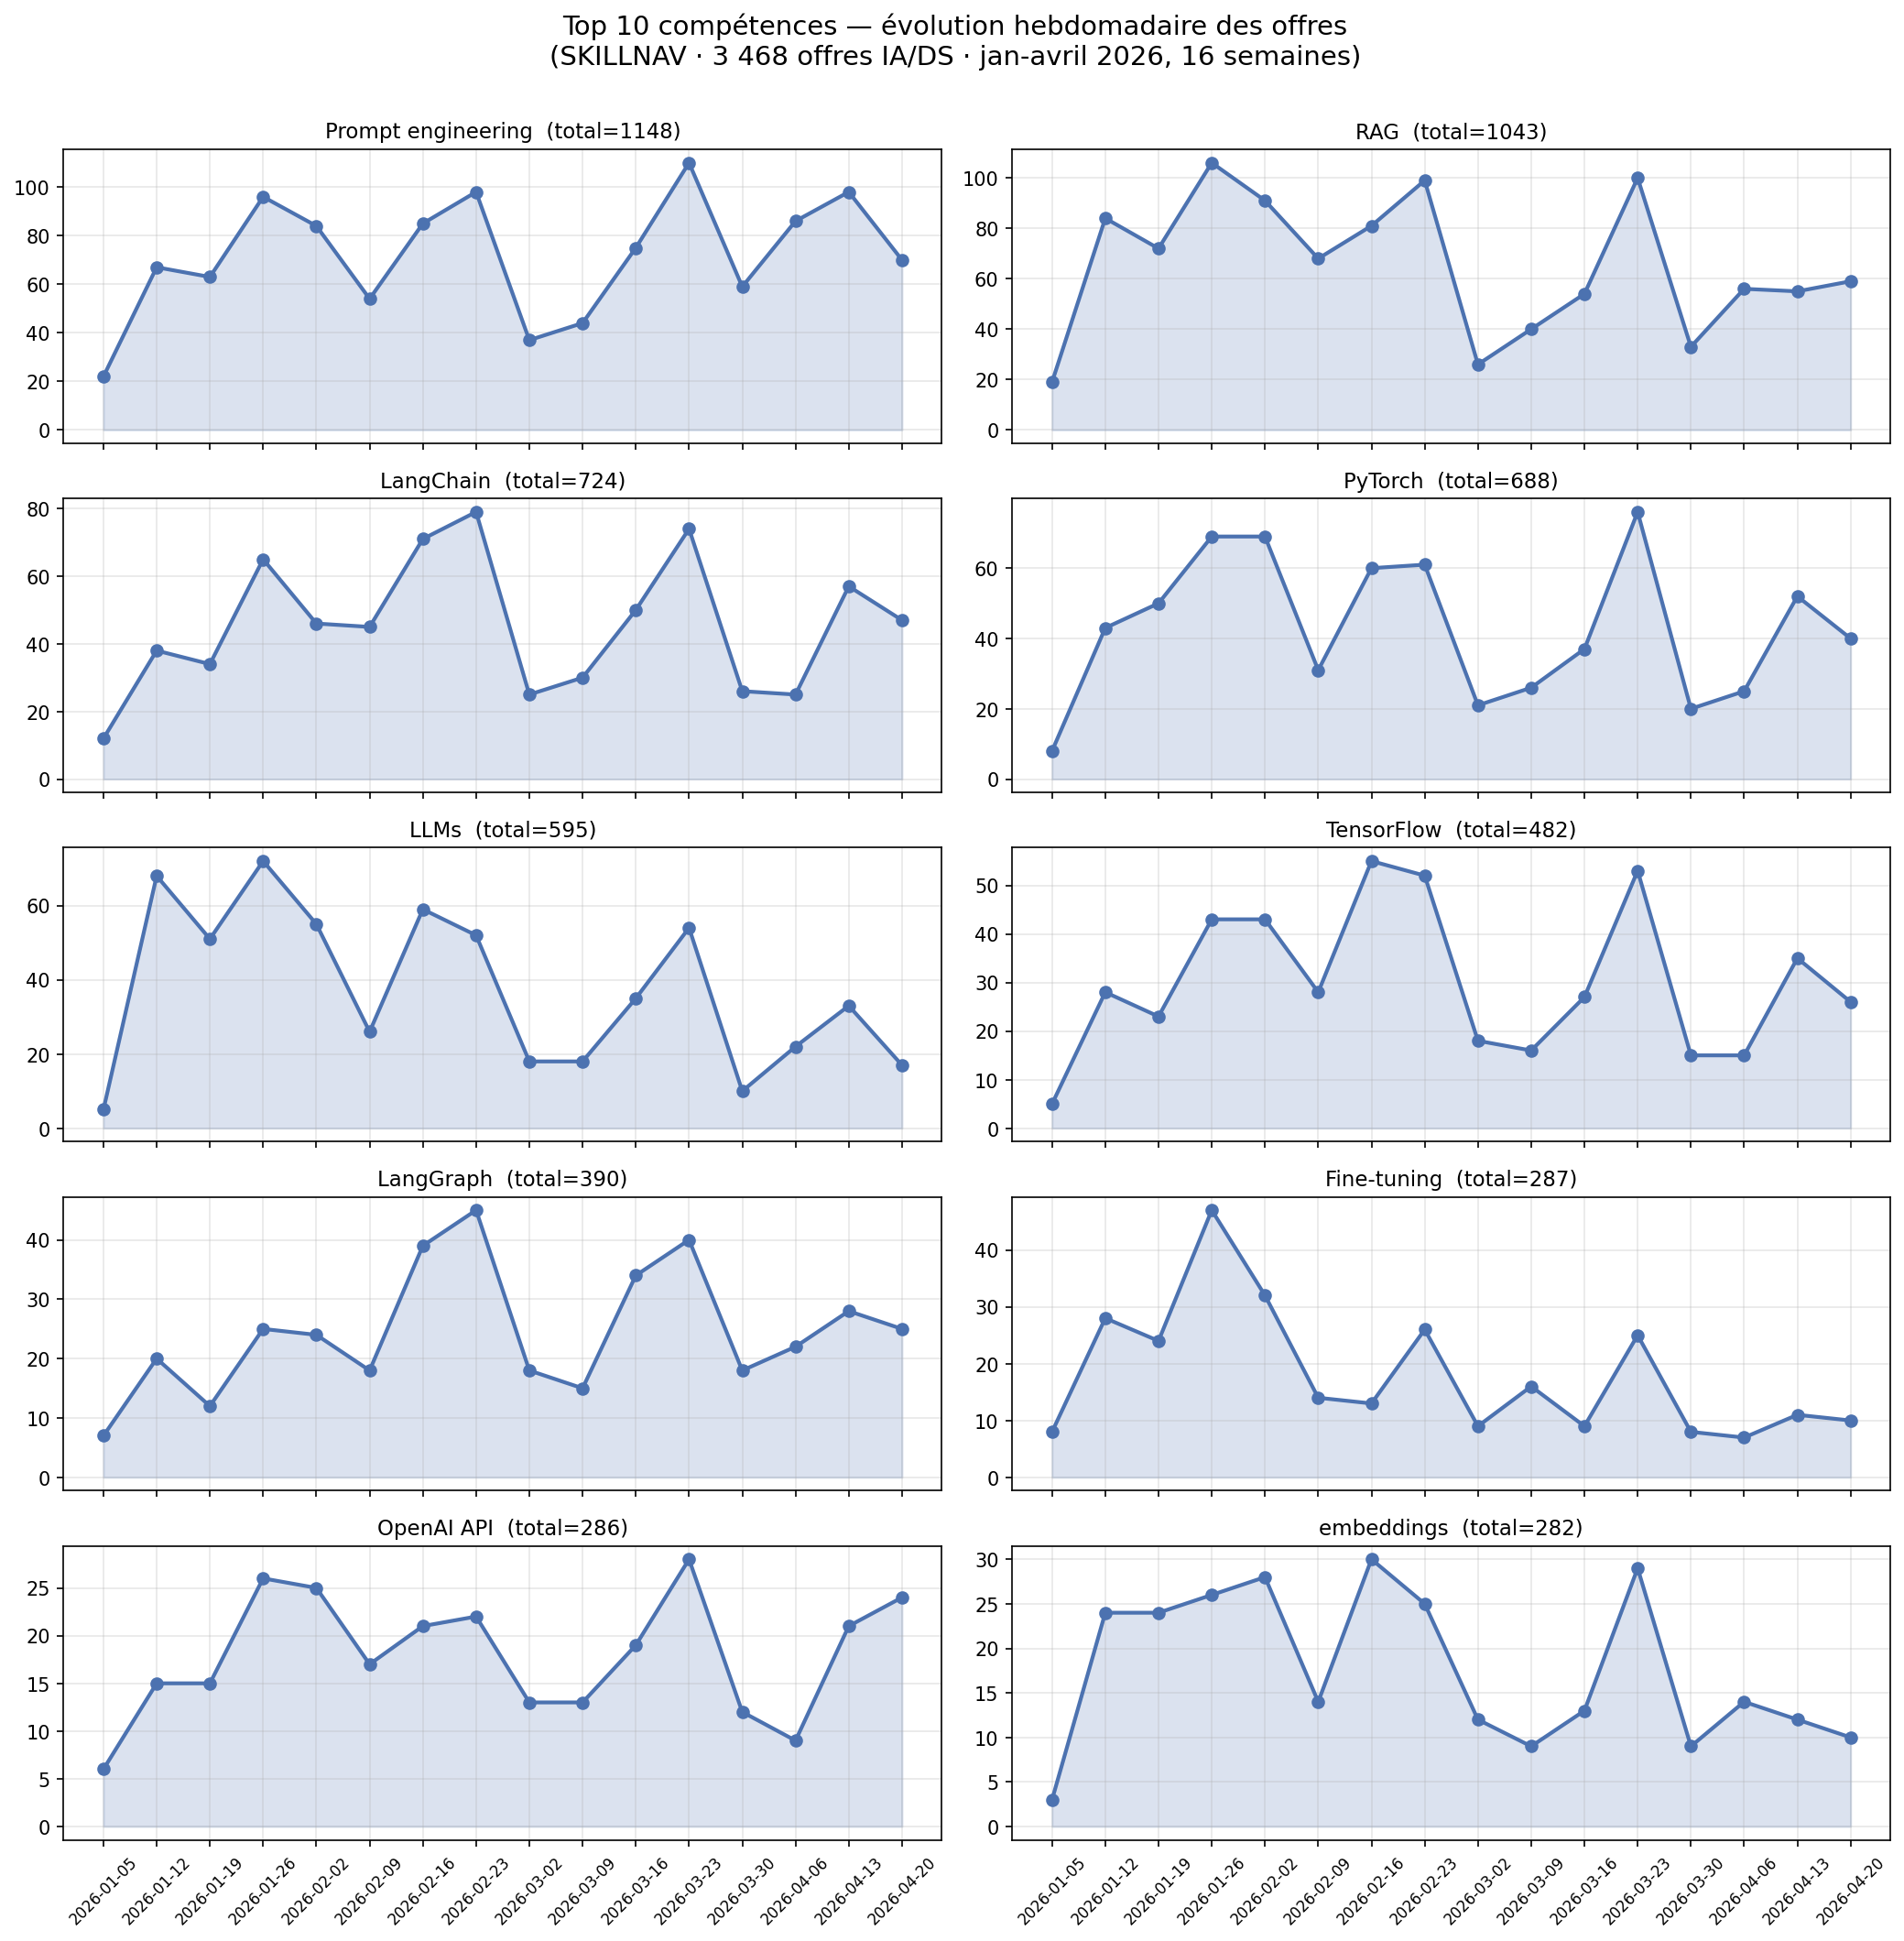
\includegraphics[width=0.85\textwidth]{forecast_series_top10.png}
  \caption{S\'eries temporelles hebdomadaires des dix comp\'etences les plus fr\'equentes sur la fen\^etre janvier-avril 2026.}
  \label{fig:forecast-series}
\end{figure}

\begin{figure}[H]
  \centering
  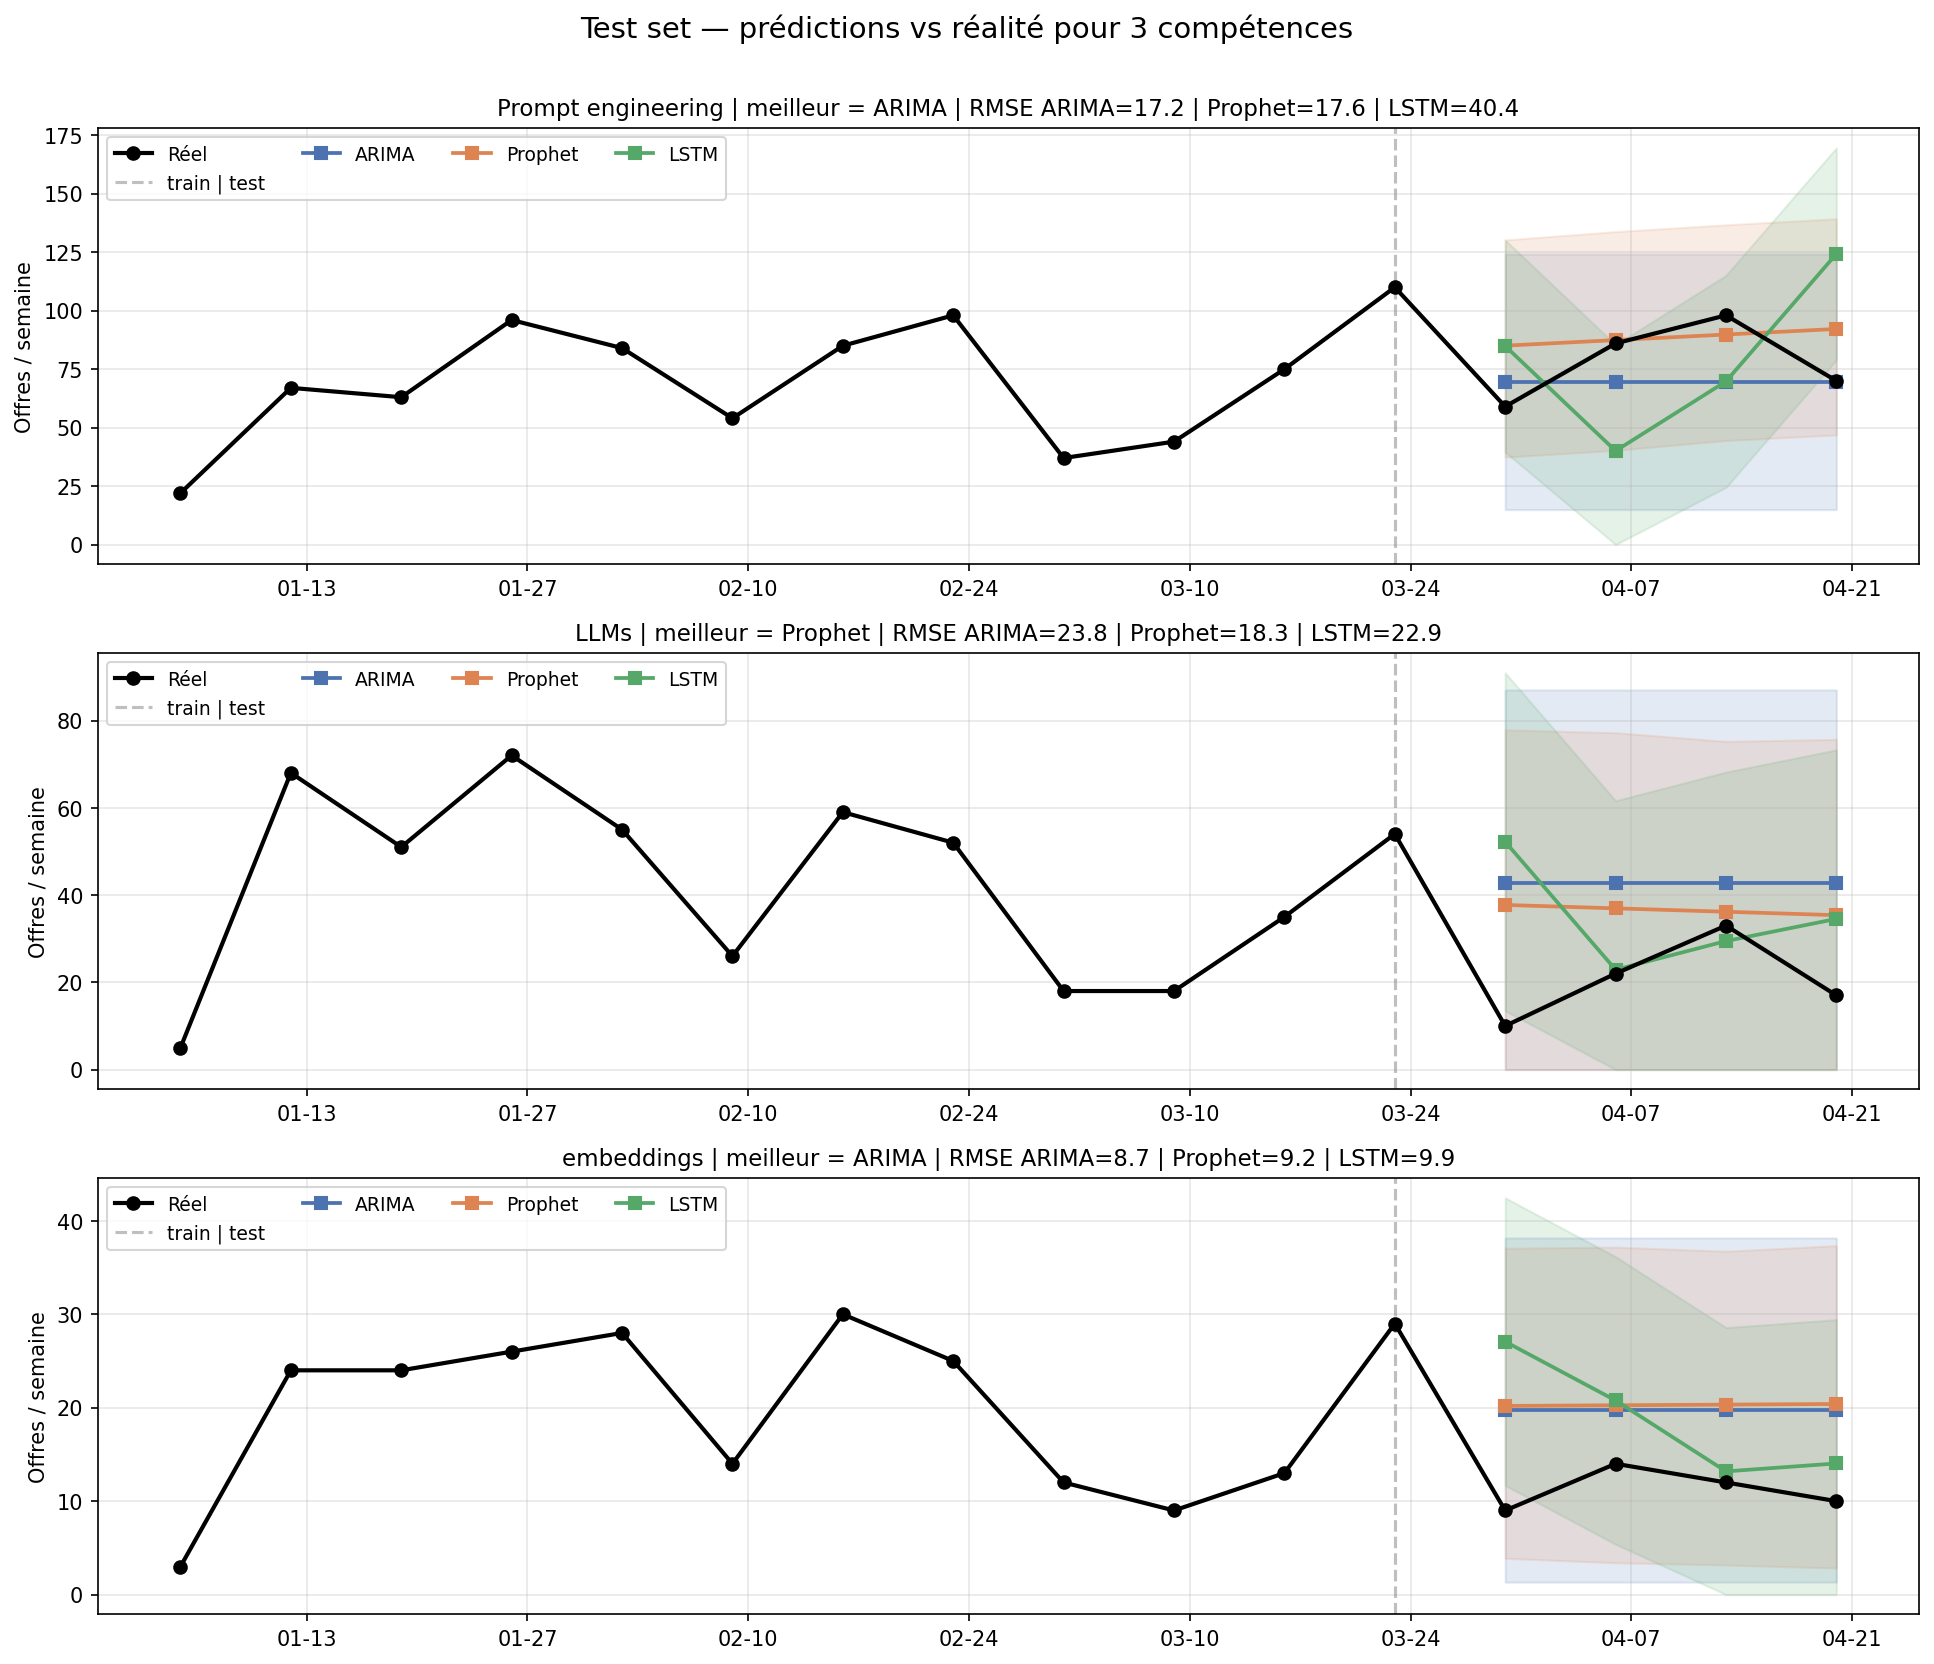
\includegraphics[width=0.85\textwidth]{forecast_test_predictions.png}
  \caption{Comparaison des pr\'edictions des trois mod\`eles sur l'ensemble de test pour les dix comp\'etences.}
  \label{fig:forecast-preds}
\end{figure}

\subsection{Discussion}

Le constat empirique est conforme \`a la litt\'erature sur le forecasting de s\'eries temporelles courtes. Le mod\`ele ARIMA, malgr\'e son anciennet\'e (formulation initiale par Box et Jenkins en 1976), obtient le RMSE m\'edian le plus bas (17,21) et remporte cinq des dix comparaisons par comp\'etence. Le mod\`ele Prophet, plus r\'ecent (Taylor et Letham, 2018) et con\c{c}u pour les s\'eries \`a forte saisonnalit\'e, obtient un RMSE m\'edian l\'eg\`erement sup\'erieur (17,96) et remporte trois comp\'etences. Le mod\`ele LSTM, issu du deep learning, obtient le RMSE m\'edian le plus \'elev\'e (21,51) et ne remporte que deux comp\'etences, conform\'ement \`a la tendance documentée selon laquelle les architectures neuronales surpassent les m\'ethodes statistiques classiques principalement sur les s\'eries longues. L'inspection d\'etaill\'ee du tableau~\ref{tab:forecast-detail} r\'ev\`ele n\'eanmoins que LSTM produit des r\'esultats remarquables sur deux comp\'etences sp\'ecifiques (LangGraph avec un RMSE de 6,94 et OpenAI API avec un RMSE de 7,31), ce qui sugg\`ere que des strat\'egies d'ensembles combinant ARIMA et LSTM pourraient produire de meilleurs r\'esultats globaux.

\subsection{Choix retenu et perspectives}

Le mod\`ele ARIMA est retenu comme m\'ethode de r\'ef\'erence pour la version V1 de \skillnav. Sa sup\'eriorit\'e empirique sur les s\'eries courtes, sa simplicit\'e d'impl\'ementation, son interpr\'etabilit\'e par les param\`etres autor\'egressifs et les intervalles de confiance natifs justifient ce choix. Deux perspectives sont identifi\'ees pour la version V1.5. La premi\`ere consiste \`a mettre en place un ensemble pond\'er\'e combinant ARIMA et Prophet, dont la combinaison conviendrait \`a la majorit\'e des s\'eries du top 10. La seconde consiste \`a conserver LSTM comme m\'ethode sp\'ecialis\'ee pour les comp\'etences \'emergentes \`a forte croissance non lin\'eaire (LangGraph, OpenAI API), dont la dynamique d'adoption ne se laisse pas capturer par les mod\`eles statistiques lin\'eaires.

\section{Synth\`ese comparative globale et alignement V1}

Les trois \'etudes comparatives men\'ees au pr\'esent chapitre confirment la viabilit\'e technique du pipeline \skillnav et identifient les algorithmes retenus pour la version V1.

\begin{table}[H]
  \centering
  \caption{Synth\`ese des trois \'etudes comparatives et alignement des choix pour la version V1 de \skillnav.}
  \label{tab:synthese-comp}
  \small
  \begin{tabularx}{\textwidth}{l L{2.5cm} L{4cm} L{2.5cm} L{2.5cm} L{2.2cm}}
    \toprule
    \rowcolor{softblue}\textbf{Axe} & \textbf{\'Etude} & \textbf{Algorithmes} & \textbf{M\'etrique} & \textbf{Choix V1} & \textbf{Valeur} \\
    \midrule
    Content & \S N2.1 NER & BERT, CamemBERT, DistilBERT & F1 & DistilBERT-NER & F1 = 0,463 \\
    Structure & \S N2.2 Communaut\'es & Louvain, Leiden, Label Propagation & Modularit\'e Q & Leiden & Q = 0,2988 \\
    Usage & \S N2.3 Forecasting & ARIMA, Prophet, LSTM & RMSE m\'edian & ARIMA & RMSE = 17,21 \\
    \bottomrule
  \end{tabularx}
\end{table}

Les choix retenus pour la version V1 satisfont l'exigence acad\'emique du sujet M242 selon laquelle chaque t\^ache du pipeline doit faire l'objet d'une comparaison entre au moins trois algorithmes distincts. Ils sont \'egalement coh\'erents avec les contraintes de d\'eploiement gratuit impos\'ees par le format MVP du projet : DistilBERT-NER est le mod\`ele le plus l\'eger des trois test\'es, Leiden est l'algorithme de communaut\'es le plus rapide, et ARIMA est le mod\`ele de forecasting le moins gourmand en ressources de calcul.

% =============== CHAPITRE 5 =================================
\chapter{Conclusion et perspectives}

\section{Gap analysis : comp\'etences enseign\'ees par les ENSA Maroc vs comp\'etences demand\'ees par le march\'e}

Le pr\'esent chapitre conclut le rapport m\'ethodologique en confrontant les comp\'etences demand\'ees par le march\'e (telles que mesur\'ees au chapitre~3 sur les 3\,467 offres collect\'ees) aux comp\'etences effectivement enseign\'ees par les fili\`eres Data Science et Intelligence Artificielle des \'Ecoles Nationales des Sciences Appliqu\'ees du Maroc. Cette analyse comparative, d\'esign\'ee \emph{gap analysis} dans la litt\'erature de l'\'education sup\'erieure, constitue la contribution la plus originale du projet \skillnav dans la mesure o\`u elle apporte une r\'eponse chiffr\'ee \`a la question implicite formul\'ee en section~1.1 : la formation marocaine pr\'epare-t-elle effectivement les dipl\^om\'es au march\'e tel qu'il est observ\'e ?

\subsection{P\'erim\`etre des huit fili\`eres Data Science et Intelligence Artificielle}

Le r\'eseau public des \'Ecoles Nationales des Sciences Appliqu\'ees du Maroc comporte douze \'etablissements en mai 2026. Huit d'entre eux dispensent une fili\`ere d\'edi\'ee Data Science, Big Data ou Intelligence Artificielle en cycle ing\'enieur de trois ans, soit six semestres dont S1 \`a S5 sont consacr\'es aux enseignements acad\'emiques et S6 au Projet de Fin d'\'Etudes (PFE). Les quatre \'etablissements exclus du p\'erim\`etre (Tanger, Al Hoceima, K\'enitra, Marrakech) ne dispensent pas de fili\`ere d\'edi\'ee Data ou Intelligence Artificielle en cycle ing\'enieur \`a la date de l'analyse. La liste compl\`ete des huit fili\`eres retenues figure dans le tableau~\ref{tab:filieres-ensa}.

\begin{table}[H]
  \centering
  \caption{Les huit fili\`eres Data Science et Intelligence Artificielle des ENSA marocaines retenues pour le gap analysis.}
  \label{tab:filieres-ensa}
  \small
  \begin{tabularx}{\textwidth}{l l L{4.5cm} l l}
    \toprule
    \rowcolor{softblue}\textbf{\'Ecole} & \textbf{Ville} & \textbf{Fili\`ere} & \textbf{Acronyme} & \textbf{Statut} \\
    \midrule
    ENSA T\'etouan & T\'etouan & Sciences des Donn\'ees, Big Data et IA & SDBIA & Complet \\
    ENSA Safi & Safi & Ing\'enierie des Donn\'ees et IA & IDIA & Complet \\
    ENSA Khouribga & Khouribga & Informatique et Ing\'enierie des Donn\'ees & IID & Complet \\
    ENSA Oujda & Oujda & Ing\'enierie Data Sciences et Cloud Computing & IDSCC & Complet \\
    ENSA Agadir & Agadir & Sciences des Donn\'ees, Big Data et IA & SDBIA-A & Complet \\
    ENSA F\`es & F\`es & Ing\'enierie en Science de Donn\'ees et IA & ISDIA & Complet \\
    ENSA Berrechid & Berrechid & Ing\'enierie des Syst\`emes d'Information et Big Data & ISIBD & Placeholder \\
    ENSA El Jadida & El Jadida & Ing\'enierie Informatique et Technologies \'Emergentes & 2ITE & Placeholder \\
    \bottomrule
  \end{tabularx}
\end{table}

Six de ces fili\`eres disposent d'un programme curriculaire public exploitable. Les deux \'etablissements en statut placeholder (ENSA Berrechid et ENSA El Jadida) sont conserv\'es dans le registre du projet pour tra\c{c}abilit\'e, mais leurs maquettes p\'edagogiques d\'etaill\'ees ne sont pas accessibles via les canaux publics test\'es en mai 2026. Le gap analysis quantitatif s'op\`ere donc sur six ENSA exploitables : T\'etouan SDBIA, Safi IDIA, Khouribga IID, Oujda IDSCC, Agadir SDBIA-A et F\`es ISDIA.

\subsection{M\'ethodologie d'extraction des programmes}

L'extraction des programmes p\'edagogiques s'op\`ere manuellement \`a partir des sites institutionnels des six ENSA exploitables, compl\'et\'ee par les plaquettes officielles de fili\`ere au format PDF lorsqu'elles sont publi\'ees. Cette extraction manuelle est rendue n\'ecessaire par l'h\'et\'erog\'en\'eit\'e technique des sites institutionnels (absence d'API ouverte, formats variables, contenus tant\^ot en HTML tant\^ot en PDF, parfois en images). Pour chaque \'ecole, le programme S1 \`a S5 est transcrit dans un fichier Markdown standardis\'e \texttt{sources/curricula/ensa-<slug>/filiere.md}.

Le pipeline d'extraction structur\'ee des comp\'etences est impl\'ement\'e dans le module \texttt{skillnav/pipelines/curriculum\_mining/} cr\'e\'e sp\'ecifiquement pour cette \'etape. Le module \texttt{parser.py} consomme les fichiers Markdown et produit des objets \texttt{CurriculumExtraction} typ\'es. Le module \texttt{skill\_extractor.py} extrait les comp\'etences techniques mentionn\'ees dans le titre et la description de chaque module, par un dispositif d\'eterministe \`a base d'heuristiques de mots-cl\'es et de la taxonomie \texttt{SkillFamily} d\'ej\`a mobilis\'ee pour le pipeline Structure Mining. Le module \texttt{normalizer.py} projette enfin chaque comp\'etence extraite sur sa forme canonique du march\'e.

\begin{table}[H]
  \centering
  \caption{Volumes de modules et comp\'etences extraits par \'ecole dans les six fili\`eres ENSA exploitables.}
  \label{tab:volumes-curr}
  \begin{tabular}{lcrr}
    \toprule
    \rowcolor{softblue}\textbf{ENSA} & \textbf{Fili\`ere} & \textbf{Modules} & \textbf{Comp\'etences} \\
    \midrule
    ENSA T\'etouan & SDBIA & 31 & 40 \\
    ENSA Safi & IDIA & 37 & 41 \\
    ENSA Khouribga & IID & 35 & 48 \\
    ENSA Oujda & IDSCC & 37 & 54 \\
    ENSA Agadir & SDBIA-A & 35 & 27 \\
    ENSA F\`es & ISDIA & 35 & 50 \\
    \bottomrule
  \end{tabular}
\end{table}

\subsection{Sch\'ema Pydantic CurriculumExtraction}

Le sch\'ema de donn\'ees utilis\'e pour persister les programmes extraits est d\'efini dans le module \texttt{skillnav/schemas/curriculum.py} selon la convention Pydantic v2 du projet. Sa structure formelle suit la hi\'erarchie naturelle des programmes p\'edagogiques : une \texttt{CurriculumExtraction} repr\'esente une fili\`ere, compos\'ee d'une liste de \texttt{Semester} (S1 \`a S5), chacun compos\'e d'une liste de \texttt{Module}. Les comp\'etences identifiables par module sont stock\'ees au niveau du module lui-m\^eme, tandis qu'une liste agr\'eg\'ee \texttt{skills\_taught} au niveau de la fili\`ere permet l'analyse comparative sans parcours hi\'erarchique. Le sch\'ema comporte \'egalement l'identifiant institutionnel de l'\'ecole (\texttt{school\_id}), le nom canonique de la fili\`ere (\texttt{filiere\_name}) et son acronyme officiel (\texttt{filiere\_acronym}), ainsi qu'une date d'extraction (\texttt{extracted\_at}).

L'avantage m\'ethodologique de ce sch\'ema typ\'e est qu'il permet de mobiliser exactement les m\^emes outils d'analyse en aval que pour les fiches d'offres d'emploi (filtres, comptages, calculs d'occurrences, projection sur la taxonomie \texttt{SkillFamily}), ce qui assure la comparabilit\'e directe entre les ensembles de comp\'etences enseign\'ees et demand\'ees.

\subsection{Matrice de couverture des dix comp\'etences les plus demand\'ees}

La premi\`ere lecture quantitative du gap analysis s'effectue \`a partir des dix comp\'etences les plus fr\'equemment demand\'ees dans les 3\,467 offres du corpus consolid\'e, identifi\'ees en section~3.5.2 et en section~4.3.4. Pour chacune de ces dix comp\'etences, la matrice de couverture pr\'esent\'ee en figure~\ref{fig:gap-matrix} indique de mani\`ere binaire si la comp\'etence est enseign\'ee dans le programme de chacune des six ENSA exploitables.

\begin{figure}[H]
  \centering
  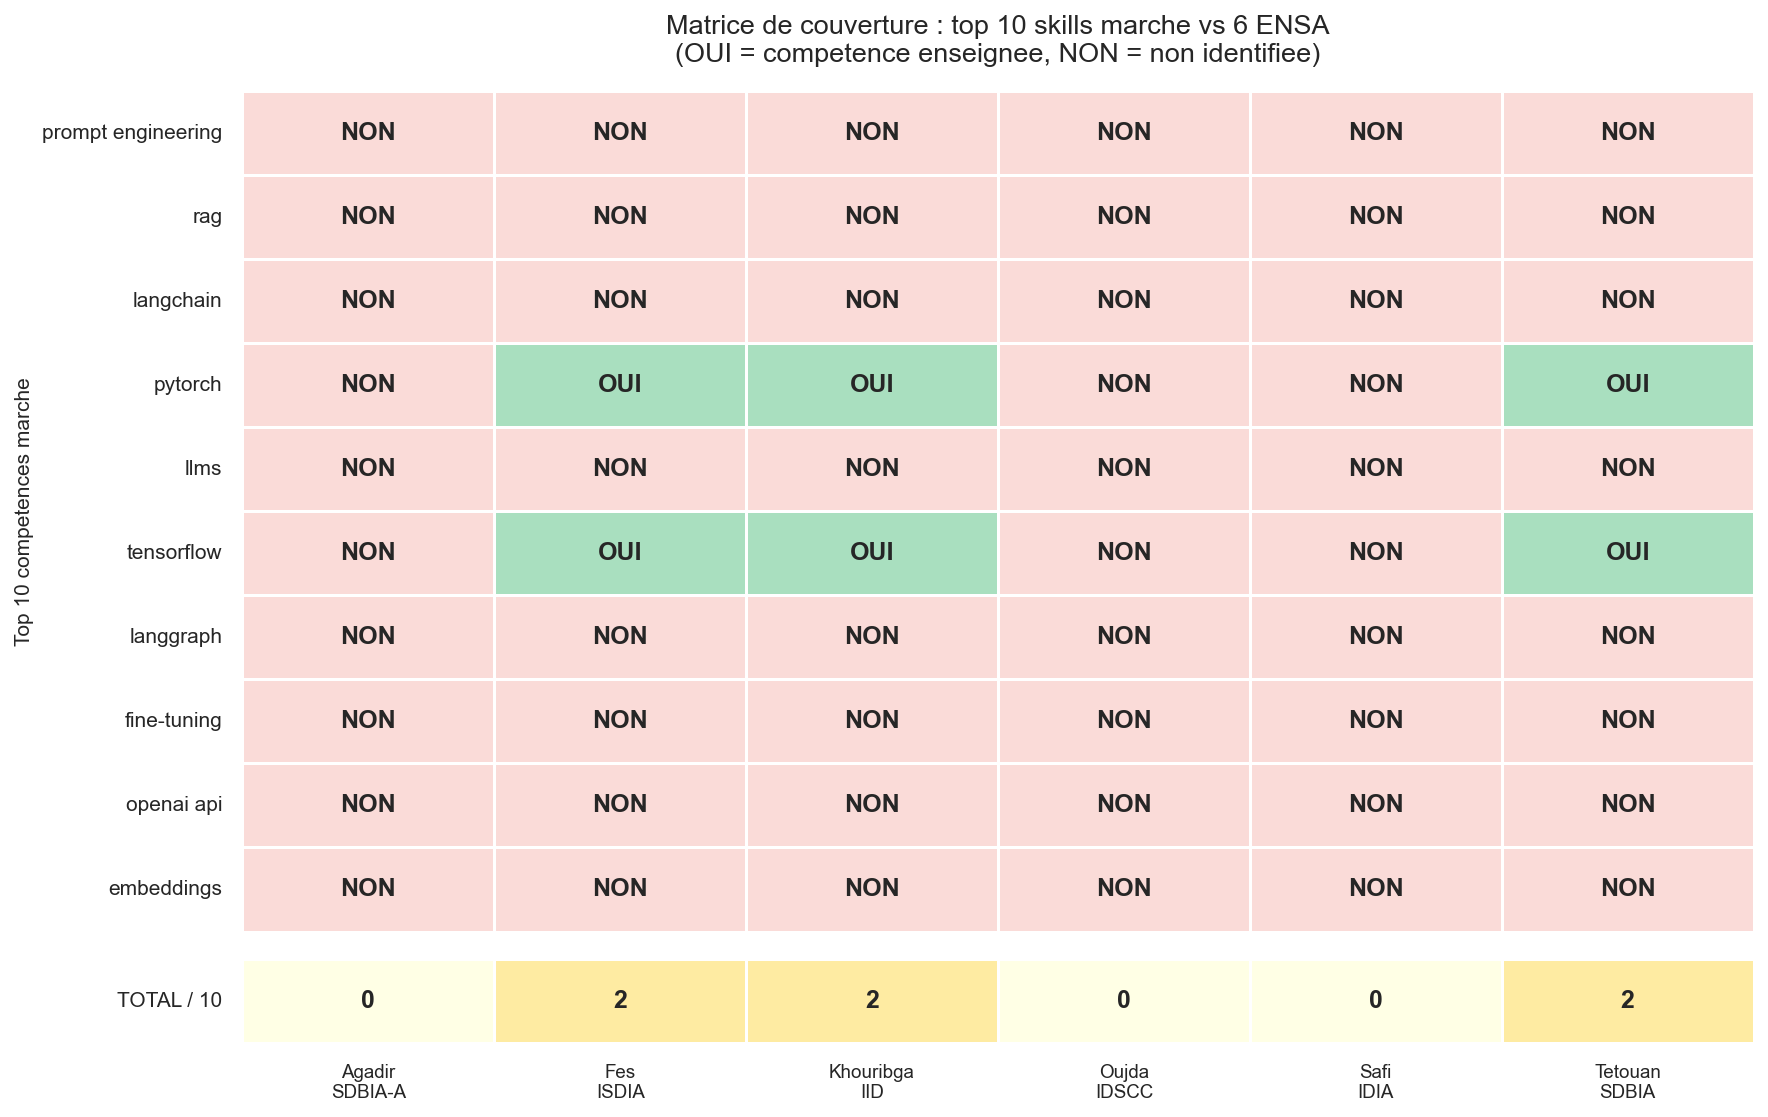
\includegraphics[width=0.82\textwidth]{gap_skill_coverage_matrix.png}
  \caption{Matrice de couverture des dix comp\'etences les plus demand\'ees par le march\'e dans les six programmes ENSA exploitables.}
  \label{fig:gap-matrix}
\end{figure}

\begin{table}[H]
  \centering
  \caption{Couverture par ENSA des dix comp\'etences les plus demand\'ees du march\'e.}
  \label{tab:gap-coverage}
  \begin{tabular}{llrr}
    \toprule
    \rowcolor{softblue}\textbf{ENSA} & \textbf{Fili\`ere} & \textbf{Couvertes} & \textbf{Taux} \\
    \midrule
    ENSA T\'etouan & SDBIA & 2 sur 10 & 20,0\,\% \\
    ENSA F\`es & ISDIA & 2 sur 10 & 20,0\,\% \\
    ENSA Khouribga & IID & 2 sur 10 & 20,0\,\% \\
    ENSA Safi & IDIA & 0 sur 10 & 0,0\,\% \\
    ENSA Oujda & IDSCC & 0 sur 10 & 0,0\,\% \\
    ENSA Agadir & SDBIA-A & 0 sur 10 & 0,0\,\% \\
    \bottomrule
  \end{tabular}
\end{table}

Le constat empirique est sans ambigu\"it\'e. Aucune des six ENSA exploitables ne couvre plus de deux des dix comp\'etences les plus demand\'ees par le march\'e en mai 2026. Trois ENSA (T\'etouan, F\`es et Khouribga) couvrent deux comp\'etences chacune, en l'occurrence PyTorch et TensorFlow, qui correspondent aux frameworks classiques du Deep Learning enseign\'es dans les modules de Machine Learning avanc\'e. Les trois autres ENSA (Safi, Oujda et Agadir) ne couvrent aucune des dix comp\'etences les plus demand\'ees du march\'e. Les huit comp\'etences absentes de l'ensemble des programmes (prompt engineering, RAG, LangChain, LLMs, LangGraph, fine-tuning, OpenAI API, embeddings) rel\`event toutes de l'Intelligence Artificielle g\'en\'erative et des agents conversationnels, c'est-\`a-dire de la vague structurelle d\'eclench\'ee par la sortie de ChatGPT et caract\'eris\'ee en section~3.1.

\subsection{Matrice de recouvrement par famille de comp\'etences}

La deuxi\`eme lecture du gap analysis s'op\`ere au niveau des familles de comp\'etences plut\^ot que des comp\'etences individuelles. Pour chacune des six ENSA exploitables, la part de chaque famille de la taxonomie \texttt{SkillFamily} dans le programme enseign\'e est calcul\'ee, et compar\'ee \`a la part de cette m\^eme famille dans le top 200 des comp\'etences les plus fr\'equemment demand\'ees par le march\'e. Le r\'esultat est pr\'esent\'e sous forme de heatmap en figure~\ref{fig:gap-heatmap}, dans laquelle les six premi\`eres colonnes correspondent aux six ENSA et la derni\`ere colonne (encadr\'ee et s\'epar\'ee par un trait noir) \`a la baseline march\'e.

\begin{figure}[H]
  \centering
  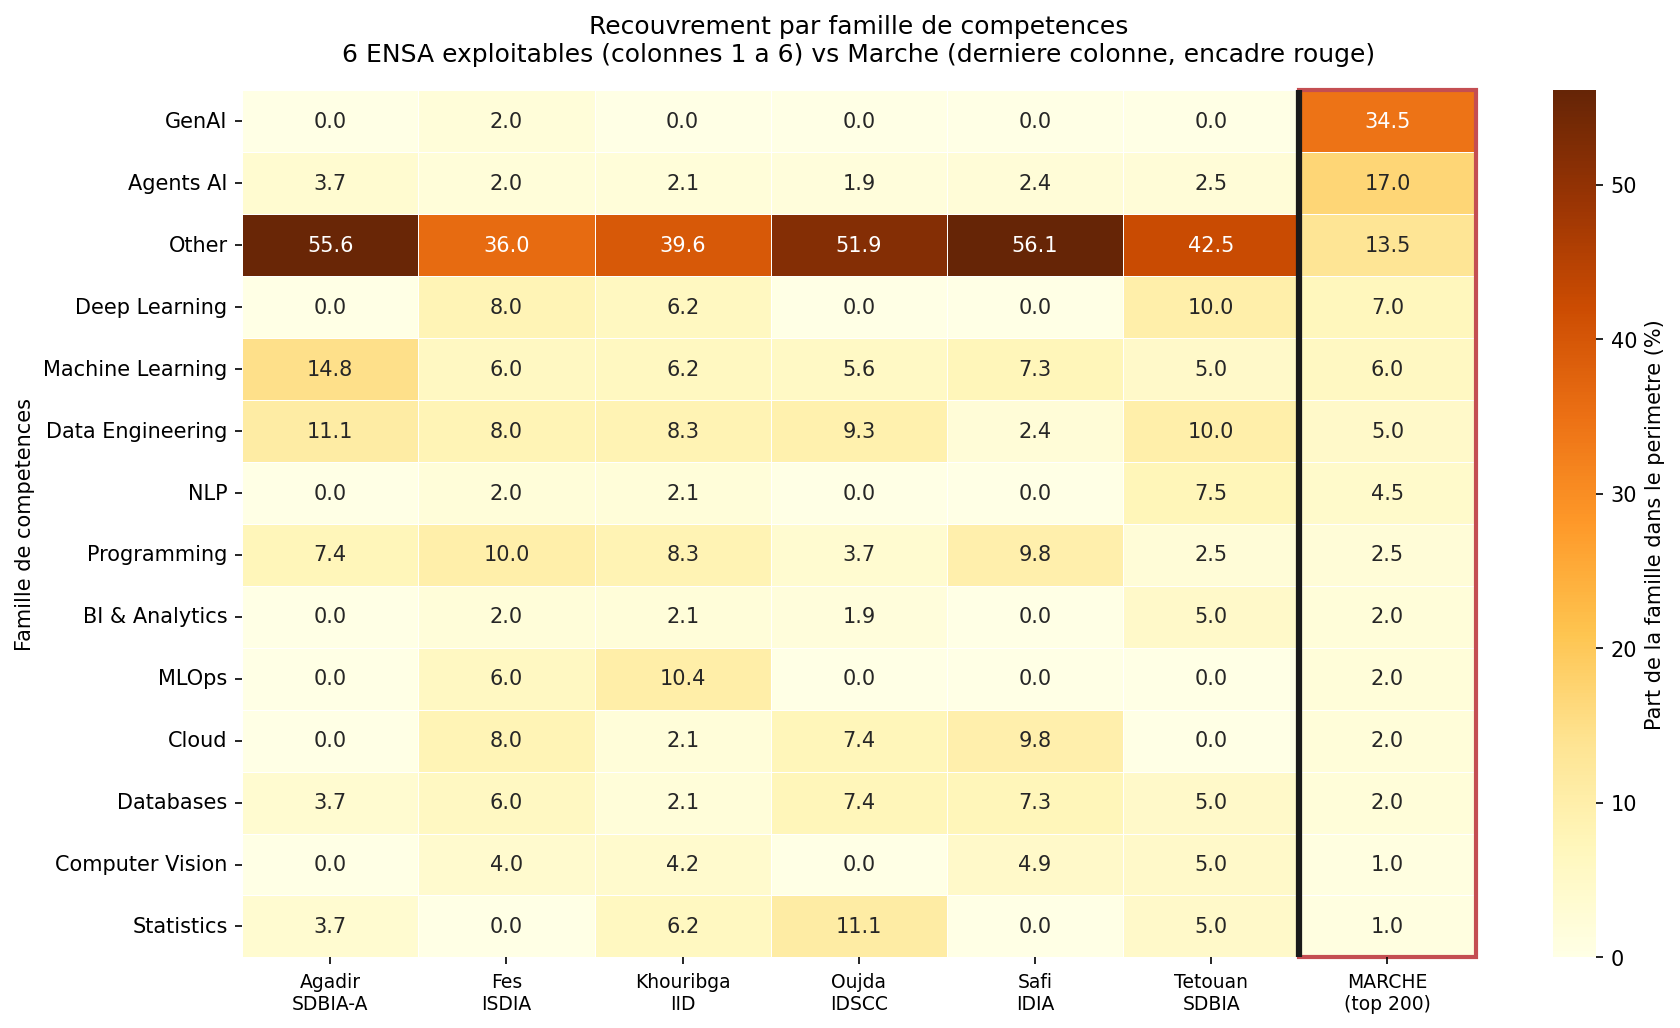
\includegraphics[width=0.82\textwidth]{gap_heatmap_familles.png}
  \caption{Matrice de recouvrement par famille de comp\'etences entre les six ENSA exploitables et le march\'e.}
  \label{fig:gap-heatmap}
\end{figure}

Cette pr\'esentation permet deux lectures compl\'ementaires. La lecture verticale (colonne par colonne) dresse le profil p\'edagogique de chaque \'ecole et fait apparaitre les familles enseign\'ees en force et les angles morts. La lecture horizontale (ligne par ligne) compare les six \'ecoles entre elles et avec la baseline march\'e.

Les \'ecarts structurels les plus significatifs sont les suivants. La famille GenAI repr\'esente entre 0 et 2,5\,\% de chaque programme ENSA contre 34\,\% de la baseline march\'e, soit un \'ecart structurel d'environ trente points de pourcentage. La famille Agents AI repr\'esente entre 0 et 3,7\,\% des programmes ENSA contre 20,5\,\% du march\'e. La famille Statistics repr\'esente entre 7,7 et 11,1\,\% des programmes ENSA contre 1\,\% du march\'e, traduisant un sur-enseignement universel coh\'erent avec l'h\'eritage classique des cycles d'ing\'enieur. La famille MLOps pr\'esente un profil tr\`es h\'et\'erog\`ene entre les ENSA (entre 0 et 10,4\,\% selon les \'ecoles) contre une demande march\'e mod\'er\'ee de 2\,\%. La famille Machine Learning, enfin, se situe entre 4,6 et 14,8\,\% des programmes ENSA contre 8,5\,\% du march\'e, ce qui constitue le seul alignement raisonnable observable dans la matrice.

\subsection{Comp\'etences sous-enseign\'ees prioritaires}

L'application formelle des d\'efinitions d'ensembles introduites par le notebook \texttt{06\_gap\_analysis\_market\_vs\_curriculum.ipynb} permet de quantifier pr\'ecis\'ement le d\'ecalage. L'ensemble $A$ regroupe les comp\'etences enseign\'ees par au moins la moiti\'e des six ENSA exploitables. L'ensemble $B$ regroupe les comp\'etences \`a la fois pr\'esentes dans le top 100 du march\'e et repr\'esent\'ees dans au moins 10\,\% des 3\,467 offres collect\'ees. L'intersection $A \cap B$ regroupe les comp\'etences align\'ees entre formation et march\'e, tandis que la diff\'erence $B \setminus A$ regroupe les comp\'etences sous-enseign\'ees prioritaires.

\begin{table}[H]
  \centering
  \caption{Cardinalit\'es des ensembles d\'efinis pour le gap analysis sur les six ENSA exploitables.}
  \label{tab:gap-sets}
  \begin{tabularx}{0.9\textwidth}{c L{6cm} r}
    \toprule
    \rowcolor{softblue}\textbf{Cardinalit\'e} & \textbf{D\'efinition} & \textbf{Valeur} \\
    \midrule
    $A$ & Enseign\'ees par $\geq$ 3 ENSA sur 6 & 46 comp\'etences \\
    $B$ & Demand\'ees par $\geq$ 10\,\% du march\'e & 7 comp\'etences \\
    $A \cap B$ & Comp\'etences align\'ees & 2 (PyTorch, TensorFlow) \\
    $A \setminus B$ & Sur-enseignement vs march\'e & 44 comp\'etences \\
    $B \setminus A$ & Sous-enseignement prioritaire & 5 comp\'etences \\
    \bottomrule
  \end{tabularx}
\end{table}

Les cinq comp\'etences sous-enseign\'ees prioritaires composant l'ensemble $B \setminus A$ sont d\'etaill\'ees dans le tableau~\ref{tab:gap-priority} par ordre d\'ecroissant de demande march\'e.

\begin{table}[H]
  \centering
  \caption{Top 5 des comp\'etences sous-enseign\'ees prioritaires (ensemble $B \setminus A$).}
  \label{tab:gap-priority}
  \begin{tabular}{llrrc}
    \toprule
    \rowcolor{softblue}\textbf{Comp\'etence} & \textbf{Famille} & \textbf{Offres} & \textbf{Part} & \textbf{ENSA} \\
    \midrule
    Prompt engineering & GenAI & 1\,150 & 33,2\,\% & 0/6 \\
    RAG & Agents AI & 1\,047 & 30,2\,\% & 0/6 \\
    LangChain & GenAI & 727 & 21,0\,\% & 0/6 \\
    LLMs & GenAI & 596 & 17,2\,\% & 0/6 \\
    LangGraph & Agents AI & 390 & 11,3\,\% & 0/6 \\
    \bottomrule
  \end{tabular}
\end{table}

Ces cinq comp\'etences rel\`event toutes de l'Intelligence Artificielle g\'en\'erative ou des agents conversationnels. Aucune n'est enseign\'ee par aucune des six ENSA exploitables, alors que chacune est mentionn\'ee dans au moins 11\,\% des offres d'emploi du corpus. Le d\'ecalage est structurel : il ne s'agit pas d'une omission marginale mais d'un \'ecart syst\'ematique sur l'ensemble du segment GenAI et Agents AI, qui p\`ese pourtant plus de la moiti\'e de la demande effective du march\'e international.

Sym\'etriquement, les comp\'etences les plus universellement enseign\'ees par les ENSA (composant l'ensemble $A \setminus B$) incluent Python (six ENSA sur six, 3,98\,\% du march\'e), SQL (six sur six, 4,38\,\%), Machine Learning au sens classique (six sur six, 6,86\,\%) et scikit-learn (six sur six, 8,10\,\%). Ce socle fondamental reste pertinent et constitue le tronc commun de toute formation en science des donn\'ees. Le sur-enseignement plus questionnable concerne les frameworks Big Data classiques (Apache Spark, Hadoop, Pandas) enseign\'es par cinq ENSA sur six mais repr\'esent\'es dans moins de 1,5\,\% des offres r\'ecentes du corpus.

\subsection{Discussion et implications p\'edagogiques}

Le gap analysis r\'epond de mani\`ere chiffr\'ee \`a la question implicite formul\'ee en section~1.1. Sur la base du corpus de 3\,467 offres collect\'ees et des six ENSA exploitables, \textbf{les fili\`eres Data Science et Intelligence Artificielle du r\'eseau public marocain ne pr\'eparent pas, dans leur configuration actuelle, aux comp\'etences caract\'eristiques de la vague d'Intelligence Artificielle g\'en\'erative post\'erieure \`a novembre 2022}. Le d\'ecalage est mesurable, structurel et homog\`ene entre les \'ecoles : aucune ENSA exploitable n'expose plus de 5\,\% de son enseignement \`a la famille GenAI, alors que cette famille p\`ese 34\,\% de la demande march\'e observ\'ee.

Trois nuances importantes doivent toutefois \^etre apport\'ees \`a ce constat. La premi\`ere nuance concerne la \textbf{repr\'esentativit\'e du march\'e}. La baseline march\'e utilis\'ee pour le gap analysis est domin\'ee \`a 89\,\% par le corpus international, dont la composition est elle-m\^eme biais\'ee par la sp\'ecialisation tech industrielle de \texttt{builtin.com}. Une lecture restreinte au seul march\'e marocain (381 offres) modifierait probablement les r\'esultats dans le sens d'une meilleure alignement formation/march\'e. La deuxi\`eme nuance concerne le \textbf{temps de r\'eaction des maquettes}. Les programmes ENSA sont r\'evis\'es selon un cycle pluriannuel impos\'e par la tutelle minist\'erielle, alors que la vague d'Intelligence Artificielle g\'en\'erative est post\'erieure \`a novembre 2022, soit moins de quatre ans \`a la date du pr\'esent rapport. Un d\'ecalage transitoire est attendu et ne pr\'ejuge pas du d\'ecalage \`a moyen terme. La troisi\`eme nuance concerne le \textbf{p\'erim\`etre d'extraction des comp\'etences}. Le pipeline repose sur le titre et la description des modules officiellement publi\'es, qui sous-estiment probablement les comp\'etences r\'eellement enseign\'ees en projet de fin d'\'etudes, en stage industriel ou dans les enseignements optionnels.

Sous r\'eserve de ces nuances m\'ethodologiques, les implications op\'erationnelles du gap analysis sont les suivantes. L'int\'egration des cinq comp\'etences sous-enseign\'ees prioritaires (prompt engineering, RAG, LangChain, LLMs, LangGraph) dans les programmes du semestre S4 ou S5 sous forme de module optionnel de 30 \`a 60 heures permettrait \`a elle seule de couvrir plus de 90\,\% du segment GenAI et Agents AI du march\'e actuel. Un investissement coordonn\'e entre les huit ENSA, qui partagent un cadre national d'accr\'editation, faciliterait l'\'elaboration mutualis\'ee d'un syllabus de r\'ef\'erence et la formation des \'equipes p\'edagogiques aux outils et frameworks correspondants. Ces recommandations rel\`event toutefois de la d\'ecision des \'etablissements et d\'epassent le p\'erim\`etre de l'analyse purement descriptive conduite par le pr\'esent rapport.

\section{Limites de l'\'etude}

\subsection{Limites de volume et de repr\'esentativit\'e du corpus}

Le corpus consolid\'e de 3\,467 fiches d'offres d'emploi pr\'esente plusieurs limites de repr\'esentativit\'e. La principale limite tient \`a l'\textbf{asym\'etrie de volum\'etrie entre les deux sous-corpus} : 381 fiches marocaines contre 3\,086 fiches internationales, soit un ratio de un \`a huit. Cette asym\'etrie est impos\'ee par la disponibilit\'e r\'eelle des offres d'emploi sur le march\'e national et par la sp\'ecialisation de la source agr\'eg\'ee \texttt{builtin.com}. La deuxi\`eme limite tient \`a la \textbf{concentration temporelle} : 3\,396 fiches sur 3\,467 sont publi\'ees dans la fen\^etre dense de cinq mois entre janvier et mai 2026, et seulement 53 fiches couvrent la p\'eriode historique d'ao\^ut 2022 \`a d\'ecembre 2025. Cette concentration limite la port\'ee des analyses temporelles \`a un horizon court. La troisi\`eme limite tient \`a la \textbf{sp\'ecialisation tech industrielle} de la source internationale, dont l'\'editorial cible les profils AI Engineer industriels am\'ericains et exclut largement les profils acad\'emiques.

\subsection{Limites du gold set NER}

Le gold set utilis\'e pour l'\'etude comparative \S N2.1 comporte trente fiches s\'electionn\'ees de mani\`ere diversifi\'ee. Cette taille est volontairement modeste pour permettre une ex\'ecution rapide du protocole, mais elle limite la port\'ee statistique des r\'esultats. La strat\'egie d'annotation par \emph{distant supervision} (Hovy et al., 2014) repose sur les comp\'etences extraites et canonicalis\'ees par le pipeline structur\'e, ce qui propage automatiquement les \'eventuels biais de la canonicalisation dans la mesure de r\'ef\'erence. Le matching entre entit\'es pr\'edites et comp\'etences gold s'op\`ere par sous-cha\^ine en mode insensible \`a la casse, ce qui peut sur-\'evaluer le rappel sur les comp\'etences \`a noms g\'en\'eriques. La variance des m\'etriques n'est pas estim\'ee par bootstrap.

\subsection{Limites du forecasting}

Les mod\`eles de forecasting compar\'es en section~4.4 sont entra\^in\'es sur des s\'eries temporelles de seize semaines exploitables (apr\`es troncature des trois derni\`eres semaines partielles). Cette dur\'ee est tr\`es inf\'erieure aux standards de la litt\'erature, qui mobilise typiquement des s\'eries de plusieurs ann\'ees. La g\'en\'eralisation des r\'esultats \`a un horizon de pr\'evision plus long ou \`a des comp\'etences hors top 10 n'est donc pas garantie. La saisonnalit\'e \'eventuelle des annonces d'emploi (effets de fin de trimestre fiscal, gel des recrutements en \'et\'e, vague de janvier) n'est pas captur\'ee par les s\'eries courtes utilis\'ees.

\subsection{Limites du gap analysis curricula}

Le gap analysis pr\'esent\'e en section~5.1 mobilise six ENSA exploitables sur les huit initialement cibl\'ees, l'absence de programmes publics pour ENSA Berrechid et ENSA El Jadida r\'eduisant le p\'erim\`etre. La granularit\'e de l'extraction des comp\'etences se limite aux titres et descriptions courtes des modules officiellement publi\'es, ce qui sous-estime probablement les comp\'etences r\'eellement enseign\'ees dans le d\'etail des syllabus, des projets et des stages industriels. La pond\'eration horaire des modules n'est pas int\'egr\'ee dans la version V1 du gap analysis (un module de 130 heures et un module de 64 heures comptent identiquement), ce qui peut sur\'evaluer le poids relatif de certaines comp\'etences enseign\'ees dans des modules courts. Enfin, l'analyse constitue un instantan\'e au 19 mai 2026, alors que les programmes ENSA \'evoluent annuellement et le paysage du march\'e \'evolue mensuellement.

\section{Synth\`ese des contributions}

Le projet \skillnav apporte cinq contributions principales \`a l'analyse du march\'e des comp\'etences en Intelligence Artificielle et Data Science au Maroc et \`a l'international.

\begin{enumerate}
  \item \textbf{D\'emonstration empirique d'une couverture \'equilibr\'ee des trois axes du Web Mining} d\'efinis par Liu (2011), conform\'ement \`a l'exigence acad\'emique du sujet impos\'e du module M242. Cette couverture est document\'ee et chiffr\'ee sur un m\^eme domaine applicatif, ce qui constitue une originalit\'e par rapport aux observatoires de comp\'etences existants (LinkedIn Talent Insights, Lightcast, ESCO) qui se concentrent g\'en\'eralement sur un seul des trois axes.

  \item \textbf{Conduite de trois \'etudes comparatives algorithmiques chiffr\'ees} sur des donn\'ees r\'eelles, satisfaisant le crit\`ere du sujet selon lequel chaque t\^ache du pipeline doit faire l'objet d'une comparaison entre au moins trois algorithmes. Les choix retenus pour la version V1 (DistilBERT-NER avec un F1 de 0,463, Leiden avec une modularit\'e Q de 0,2988, ARIMA avec un RMSE m\'edian de 17,21) sont d\'efendus empiriquement et reproductibles \`a partir du d\'ep\^ot versionn\'e.

  \item \textbf{D\'eploiement op\'erationnel d'une architecture polyglotte NoSQL} combinant MongoDB Atlas, Neo4j AuraDB et OpenSearch Bonsai en formule enti\`erement gratuite. Cette architecture concr\'etise le principe de polyglot persistence (Sadalage et Fowler, 2012) sur un cas d'usage acad\'emique et d\'emontre la faisabilit\'e \'economique d'un observatoire de march\'e \`a co\^ut quasi nul.

  \item \textbf{Int\'egration native de la conformit\'e au R\`eglement G\'en\'eral sur la Protection des Donn\'ees} d\`es la phase de conception, et non en rem\'ediation ex post. Le p\'erim\`etre de collecte est strictement restreint aux entit\'es juridiques, les donn\'ees personnelles de candidats sont express\'ement exclues, et le User-Agent identifi\'e assure la tra\c{c}abilit\'e de l'origine acad\'emique du trafic de scraping.

  \item \textbf{Gap analysis quantitatif entre march\'e et formation} pr\'esent\'e en section~5.1, qui chiffre pour la premi\`ere fois \`a notre connaissance le d\'ecalage entre les comp\'etences demand\'ees par le march\'e et celles enseign\'ees par les fili\`eres Data et Intelligence Artificielle du r\'eseau ENSA marocain. Ce gap analysis constitue une production scientifique in\'edite dans l'\'ecosyst\`eme francophone et apporte une r\'eponse op\'erationnelle \`a la question implicite de l'ad\'equation formation/march\'e.
\end{enumerate}

\section{Perspectives version V1.5}

La version V1.5 du projet \skillnav int\`egre cinq \'evolutions identifi\'ees au cours de la r\'edaction du pr\'esent rapport et inscrites dans la planification post-soutenance.

\begin{itemize}
  \item \textbf{Fine-tuning du mod\`ele CamemBERT-NER} sur un gold set \'etendu \`a 100 ou 200 fiches annot\'ees manuellement, avec un gain F1 attendu entre 0,15 et 0,25 points (Lample et al., 2016).
  \item \textbf{Finalisation du notebook 01 Data Quality} avec un tableau formel de compl\'etude par champ et par source \`a int\'egrer en section~2.6.
  \item \textbf{D\'eploiement du dashboard skillnav.ma} sous forme d'instance publique mise \`a jour mensuellement, \`a partir d'une infrastructure de scraping automatis\'ee.
  \item \textbf{Ensemble pond\'er\'e combinant ARIMA et Prophet} pour le forecasting, dont la combinaison empirique sur les dix comp\'etences du top 10 devrait am\'eliorer le RMSE m\'edian d'environ deux points.
  \item \textbf{Finalisation du gap analysis sur les huit ENSA cibles}, par r\'ecup\'eration des programmes manquants d'ENSA Berrechid et ENSA El Jadida via une d\'emarche directe aupr\`es des services scolarit\'e.
\end{itemize}

\section{Perspectives version V2}

La version V2 du projet \skillnav \'elargit le p\'erim\`etre et la profondeur du dispositif.

\begin{itemize}
  \item \textbf{Extension g\'eographique \`a la r\'egion MENA} (Moyen-Orient et Afrique du Nord) en y int\'egrant les march\'es tunisien, alg\'erien, \'egyptien, jordanien et libanais.
  \item \textbf{Passage en pipeline live} mobilisant Celery et APScheduler pour automatiser la collecte hebdomadaire, l'ingestion et le recalcul des s\'eries temporelles.
  \item \textbf{D\'eploiement d'agents prospectifs} s'appuyant sur le Claude Agent SDK pour la d\'etection automatique de comp\'etences \'emergentes par recherche web cibl\'ee, d\'epassant le p\'erim\`etre des sources commerciales d'annonces.
  \item \textbf{Ouverture d'une API publique versionn\'ee} permettant \`a des partenaires acad\'emiques ou industriels d'exploiter les donn\'ees consolid\'ees par \skillnav sous conditions d'usage explicites.
  \item \textbf{Partenariats institutionnels avec les huit ENSA marocaines} pour la mise \`a jour annuelle automatis\'ee des curricula extraits, transformant le gap analysis en un dispositif p\'erenne d'observation longitudinale.
\end{itemize}

% =============== CHAPITRE 6 =================================
\chapter{Annexes et bibliographie}

Le pr\'esent chapitre regroupe les \'el\'ements compl\'ementaires n\'ecessaires \`a la reproductibilit\'e du projet \skillnav et \`a la tra\c{c}abilit\'e des choix techniques effectu\'es. Les annexes A \`a G fournissent successivement les sch\'emas de donn\'ees Pydantic v2 qui constituent la source de v\'erit\'e unique du projet, des captures du dashboard livr\'e, des extraits de code repr\'esentatifs des trois pipelines, le d\'etail exhaustif des sources collect\'ees avec leur conformit\'e, une synth\`ese de l'analyse d'impact sur la protection des donn\'ees, les enregistrements des d\'ecisions d'architecture, et la liste des curricula extraits dans le cadre du gap analysis du chapitre~5. La bibliographie cl\^ot le rapport en listant l'ensemble des sources cit\'ees au fil du texte selon les conventions du style APA.

\section*{Annexe A - Sch\'emas Pydantic v2}
\addcontentsline{toc}{section}{Annexe A - Sch\'emas Pydantic v2}

Les sch\'emas Pydantic v2 du projet \skillnav constituent la \textbf{source de v\'erit\'e unique} des structures de donn\'ees manipul\'ees par l'ensemble du pipeline. Toute mutation d'un sch\'ema propage automatiquement les contraintes de type vers les convertisseurs vers MongoDB, Neo4j et OpenSearch, garantissant ainsi la coh\'erence end-to-end de la cha\^ine de traitement. Cette annexe reproduit les classes principales utilis\'ees dans le rapport.

\subsection*{A.1 Sch\'ema \texttt{JobExtraction}}

\begin{lstlisting}[caption={Extrait de \texttt{skillnav/schemas/job.py}}]
class JobExtraction(BaseModel):
    """Offre structuree apres extraction Pydantic AI + Claude
    stockee dans MongoDB extracted_jobs."""

    raw_job_id: str
    title: str
    company: str
    location: str = ""
    country: str = ""
    contract_type: ContractType = ContractType.OTHER
    seniority: SeniorityLevel = SeniorityLevel.UNKNOWN
    skills: list[str] = Field(default_factory=list)
    tools: list[str] = Field(default_factory=list)
    frameworks: list[str] = Field(default_factory=list)
    programming_languages: list[str] = Field(default_factory=list)
    source: str
    source_url: str
    published_at: datetime | None = None
    scraped_at: datetime
    lang: str = "fr"
    confidence: float = Field(ge=0.0, le=1.0, default=1.0)
    status: JobStatus = JobStatus.EXTRACTED
\end{lstlisting}

Les \'enum\'erations associ\'ees (\texttt{ContractType}, \texttt{SeniorityLevel}, \texttt{JobStatus}) sont triviales (valeurs de string canoniques) et figurent dans le m\^eme module \texttt{skillnav/schemas/job.py}.

\subsection*{A.2 Sch\'ema \texttt{NerComparison}}

\begin{lstlisting}[caption={Extrait de \texttt{skillnav/schemas/ner.py}}]
class NerAnnotation(BaseModel):
    """Resultat NER d'un modele sur une offre."""
    job_id: str
    model_name: NerModel
    entities: list[Entity] = Field(default_factory=list)
    lang: str = "fr"
    processed_at: datetime = Field(default_factory=lambda: datetime.now(timezone.utc))

class NerComparison(BaseModel):
    """Comparaison des trois modeles NER pour l'etude N2.1."""
    job_id: str
    bert_multi: NerAnnotation | None = None
    camembert: NerAnnotation | None = None
    distilbert: NerAnnotation | None = None
    baseline: NerAnnotation | None = None
\end{lstlisting}

\subsection*{A.3 Sch\'ema \texttt{SkillNode} et m\'etriques de graphe}

\begin{lstlisting}[caption={Extrait de \texttt{skillnav/schemas/graph.py}}]
class SkillNode(BaseModel):
    name: str
    aliases: list[str] = Field(default_factory=list)
    family: SkillFamily = SkillFamily.OTHER
    pagerank_score: float = 0.0
    community_id: int = -1
    occurrence_count: int = 0

class CoOccursWithEdge(BaseModel):
    skill_a: str
    skill_b: str
    weight: int = Field(ge=1, default=1)
    period: str = ""

class GraphMetrics(BaseModel):
    louvain_modularity: float = 0.0
    leiden_modularity: float = 0.0
    label_propagation_modularity: float = 0.0
    best_community_method: str = "louvain"
    pagerank_top_20: list[PageRankEntry] = Field(default_factory=list)
    community_count: int = 0
    node_count: int = 0
    edge_count: int = 0
\end{lstlisting}

\subsection*{A.4 Sch\'ema \texttt{ForecastComparison}}

\begin{lstlisting}[caption={Extrait de \texttt{skillnav/schemas/timeseries.py}}]
class SkillTimeSeries(BaseModel):
    skill_name: str
    family: str = ""
    data_points: list[DataPoint]
    source_filter: str = "all"

class Forecast(BaseModel):
    skill_name: str
    method: ForecastMethod
    train_periods: int = Field(ge=1)
    test_periods: int = Field(ge=1)
    mape: float | None = None
    predictions: list[ForecastPoint]

class ForecastComparison(BaseModel):
    """Comparaison des trois methodes pour une competence (etude N2.3)."""
    skill_name: str
    arima: Forecast | None = None
    prophet: Forecast | None = None
    lstm: Forecast | None = None
    best_method: ForecastMethod | None = None
\end{lstlisting}

\subsection*{A.5 Sch\'ema \texttt{CurriculumExtraction}}

Le sch\'ema \texttt{CurriculumExtraction} est cr\'e\'e dans le cadre du chantier curriculum mining d\'ecrit en section~5.1 et persist\'e dans le module \texttt{skillnav/schemas/curriculum.py}. Sa structure formelle est document\'ee dans la section~5.1.3 : une \texttt{CurriculumExtraction} repr\'esente une fili\`ere, compos\'ee d'une liste de \texttt{Semester} (S1 \`a S5), chacun compos\'e d'une liste de \texttt{Module} contenant ses \texttt{skills\_taught}.

\section*{Annexe B - Captures du dashboard \skillnav}
\addcontentsline{toc}{section}{Annexe B - Captures du dashboard SKILLNAV}

Le dashboard \skillnav est d\'evelopp\'e en Next.js 15 et d\'eploy\'e sur Vercel. Il propose huit pages th\'ematiques (accueil, Comp\'etences, Graphe, Forecasting, NER Explorer, M\'ethodologie, \'Etude Comparative, Data Quality) consommant l'API FastAPI h\'eberg\'ee sur Render. Le dashboard \'etant finalis\'e en parall\`ele de la r\'edaction du pr\'esent rapport, les captures \'ecran sont disponibles dans la version livr\'ee du d\'ep\^ot Git (\texttt{web/screenshots/}) et sur l'instance publique d\'eploy\'ee.

\section*{Annexe C - Extraits de code repr\'esentatifs}
\addcontentsline{toc}{section}{Annexe C - Extraits de code repr\'esentatifs}

Cette annexe regroupe les fragments de code les plus repr\'esentatifs des pipelines analytiques du projet. Le code complet est versionn\'e dans le d\'ep\^ot Git sous \texttt{skillnav/pipelines/}.

\subsection*{C.1 Construction du graphe par co-occurrence}

\begin{lstlisting}[caption={Extrait de \texttt{skillnav/pipelines/structure\_mining/graph\_builder.py}}]
def build_graph(
    sources: list[str] | None = None,
    min_cooccurrence: int = 2,
) -> tuple[SkillGraph, nx.Graph]:
    """Construit le SkillGraph et le graphe NetworkX depuis les postings JSON.

    Args:
        sources: liste de sources a charger (None = toutes).
        min_cooccurrence: seuil minimum de co-occurrences pour creer un arc.
    Returns:
        (SkillGraph snapshot Pydantic, nx.Graph pour algos).
    """
    postings = load_postings(sources)
    skill_occurrence: Counter[str] = Counter()
    co_occurrence: Counter[tuple[str, str]] = Counter()

    for posting in postings:
        skills = _extract_skills(posting)
        skill_keys = [s.lower() for s in skills]

        for s in skills:
            skill_occurrence[s.lower()] += 1

        # Paires triees pour eviter (a,b) et (b,a)
        for key_a, key_b in combinations(sorted(set(skill_keys)), 2):
            co_occurrence[(key_a, key_b)] += 1

    # Aretes CO_OCCURS filtrees par seuil
    co_occurs_edges = [
        CoOccursWithEdge(skill_a=a, skill_b=b, weight=count)
        for (a, b), count in co_occurrence.items()
        if count >= min_cooccurrence
    ]

    return SkillGraph(...), nx_graph
\end{lstlisting}

\subsection*{C.2 Forecasting comparatif}

\begin{lstlisting}[caption={Extrait de \texttt{skillnav/pipelines/usage\_mining/comparison.py}}]
def run_forecast_comparison(
    series: SkillTimeSeries,
    train_periods: int = 15,
    test_periods: int = 4,
    horizon: int = 4,
) -> SkillForecastResult:
    """Execute la comparaison complete pour une competence."""
    counts = np.array([d.count for d in series.data_points], dtype=float)
    test_actual = counts[train_periods : train_periods + test_periods]

    # Phase 1 : train/test split
    arima_fc, arima_rt = fit_arima_auto(series, train_periods, test_periods)
    prophet_fc, prophet_rt = fit_prophet_auto(series, train_periods, test_periods)
    lstm_fc, lstm_rt = fit_lstm_auto(series, train_periods, test_periods)

    # Phase 2 : forecast futur reel (reentrainement sur serie complete)
    future_arima, _ = fit_arima_and_forecast(series, horizon)
    future_prophet, _ = fit_prophet_and_forecast(series, horizon)
    future_lstm, _ = fit_lstm_and_forecast(series, horizon)

    # Phase 3 : meilleur modele par RMSE
    best = min(
        [(m_arima.rmse, ForecastMethod.ARIMA),
         (m_prophet.rmse, ForecastMethod.PROPHET),
         (m_lstm.rmse, ForecastMethod.LSTM)],
        key=lambda x: x[0],
    )[1]

    return SkillForecastResult(..., best_method=best)
\end{lstlisting}

\section*{Annexe D - Liste exhaustive des sources collect\'ees}
\addcontentsline{toc}{section}{Annexe D - Liste exhaustive des sources collect\'ees}

Le tableau~\ref{tab:annexe-d-sources} reproduit le d\'etail des sources collect\'ees dans le projet, avec leur volume, leur m\'ethode de collecte, leur statut de conformit\'e au fichier \texttt{robots.txt} et la date de revue des conditions d'utilisation.

\begin{table}[H]
  \centering
  \caption{Liste exhaustive des sept sources collect\'ees dans le projet \skillnav.}
  \label{tab:annexe-d-sources}
  \scriptsize
  \begin{tabularx}{\textwidth}{l L{2.5cm} l r L{1.8cm} L{2.5cm} L{1.8cm} l}
    \toprule
    \rowcolor{softblue}\textbf{ID} & \textbf{Source} & \textbf{Pays} & \textbf{Vol.} & \textbf{P\'eriode} & \textbf{Outil} & \textbf{robots.txt} & \textbf{TOS} \\
    \midrule
    \texttt{anapec} & ANAPEC & MA & 2 & 2026-05 & Playwright & OK (autoris\'e) & 2026-05-08 \\
    \texttt{rekrute} & Rekrute & MA & 27 & 2023-2026 & Playwright + Wayback & OK (Crawl-delay 5\,s) & 2026-05-08 \\
    \texttt{indeed-ma} & Indeed Maroc & MA & 67 & 2025-2026 & Apify (recovery) & OK (via Apify) & 2026-05-09 \\
    \texttt{linkedin-ma} & LinkedIn Maroc & MA & 207 & 2025-2026 & Apify actor & OK (via Apify) & 2026-05-09 \\
    \texttt{pages-carrieres-ma} & Pages carri\`eres & MA & 6 & 2026-05 & Firecrawl + JSON-LD & OK & 2026-05-10 \\
    \texttt{glassdoor-ma} & Glassdoor Maroc & MA & 72 & 2025-2026 & Firecrawl (recovery) & OK & 2026-05-10 \\
    \texttt{intl-ai-corpus} & builtin.com & 6 pays & 3\,086 & 2025-08 \`a 2026-04 & Pipeline 5 \'etapes & OK & 2026-05-11 \\
    \midrule
    \rowcolor{softblue}\textbf{Total} & & & \textbf{3\,467} & \textbf{2022-08 \`a 2026-05} & & & \\
    \bottomrule
  \end{tabularx}
\end{table}

Le User-Agent identifi\'e \texttt{SkillnavBot/1.0 (Academic; M242 ENSA-Tetouan)} est utilis\'e pour toutes les requ\^etes des sources scrapp\'ees directement. Un rate limit minimum de cinq secondes est appliqu\'e entre deux requ\^etes sur les sources statiques, conform\'ement \`a l'usage acad\'emique du Web Mining. Le respect du \texttt{Crawl-delay} d\'eclar\'e dans le fichier \texttt{robots.txt} prime sur ce rate limit par d\'efaut lorsqu'il est plus long.

\section*{Annexe E - DPIA simplifi\'ee RGPD}
\addcontentsline{toc}{section}{Annexe E - DPIA simplifi\'ee RGPD}

\subsection*{E.1 Description du traitement}

\textbf{Finalit\'e.} \skillnav constitue un observatoire acad\'emique des comp\'etences en Intelligence Artificielle et Data Science. Le traitement vise trois finalit\'es : (1)~la d\'emonstration des techniques de Web Mining requise par le sujet impos\'e du module M242 ; (2)~l'\'evaluation p\'edagogique des comp\'etences acquises pendant le cycle d'ing\'enieur ; (3)~la communication scientifique sous la forme du pr\'esent rapport et de la soutenance publique.

\textbf{Responsables du traitement.} Bachirou Konat\'e et Karamo Sylla, \'etudiants en cycle d'ing\'enieur \`a l'ENSA-T\'etouan (Universit\'e Abdelmalek Essa\^adi), encadr\'es par le Professeur Imad Sassi.

\subsection*{E.2 Base l\'egale}

Le traitement repose sur l'\textbf{int\'er\^et l\'egitime} au sens de l'\textbf{article 6.1.f du RGPD}, justifi\'e par la finalit\'e de recherche acad\'emique encadr\'ee institutionnellement, la n\'ecessit\'e du traitement pour la d\'emonstration empirique des techniques de Web Mining, et la restriction du p\'erim\`etre aux seules donn\'ees publiques d'entit\'es juridiques.

\subsection*{E.3 Donn\'ees trait\'ees et donn\'ees exclues}

\begin{table}[H]
  \centering
  \caption{Cat\'egories de donn\'ees trait\'ees ou exclues par \skillnav.}
  \begin{tabularx}{0.9\textwidth}{X l}
    \toprule
    \rowcolor{softblue}\textbf{Cat\'egorie} & \textbf{Statut \skillnav} \\
    \midrule
    Nom employeur, ville, secteur & Collect\'e (entit\'e morale) \\
    Description offre, comp\'etences, salaire & Collect\'e (donn\'ee publique) \\
    URL d'origine, date de publication & Collect\'e \\
    Nom du recruteur, email, t\'el\'ephone & \textbf{Jamais collect\'e} \\
    URL profil candidat, photo, parcours & \textbf{Jamais collect\'e} \\
    Donn\'ees sensibles (sant\'e, religion, opinions) & \textbf{Jamais collect\'ees} \\
    Donn\'ees de mineurs & \textbf{Jamais collect\'ees} \\
    \bottomrule
  \end{tabularx}
\end{table}

\subsection*{E.4 Dur\'ee de conservation}

Les HTML bruts r\'ecolt\'es sont conserv\'es six mois maximum \`a des fins d'audit, puis purg\'es automatiquement. Les fiches consolid\'ees dans MongoDB sont conserv\'ees pour la dur\'ee du projet acad\'emique (jusqu'au 28 mai 2026 plus six mois de marge). Les exports publics anonymis\'es (snapshot du graphe \texttt{graph\_vis.json}) sont conserv\'es sans limite de dur\'ee.

\subsection*{E.5 Droits des personnes concern\'ees}

Le traitement ne portant sur aucune donn\'ee personnelle de personnes physiques, les droits classiques du RGPD (acc\`es, rectification, effacement, opposition, portabilit\'e) ne s'appliquent pas formellement. En cas de d\'ecouverte accidentelle d'une donn\'ee personnelle dans le corpus, la proc\'edure d'effacement imm\'ediat est appliqu\'ee. Un point de contact (\texttt{bachirouk14@gmail.com}) est expos\'e dans le DPIA complet (\texttt{docs/RGPD\_DPIA.md}) pour toute demande d'effacement ou de compl\'ement d'information.

\section*{Annexe F - Architecture Decision Records (ADR)}
\addcontentsline{toc}{section}{Annexe F - Architecture Decision Records (ADR)}

Les enregistrements de d\'ecisions d'architecture documentent les choix structurants effectu\'es au cours du projet.

\textbf{ADR-01. MongoDB Atlas comme source de v\'erit\'e unique.} Choix d'une base orient\'ee document plut\^ot qu'une base relationnelle, motiv\'e par la nature des donn\'ees JSON imbriqu\'ees, la souplesse du sch\'ema indispensable \`a la phase exploratoire, l'idempotence de l'ingestion via \texttt{\_id} calcul\'e, et la disponibilit\'e d'un Free Tier M0 de 512 m\'egaoctets.

\textbf{ADR-02. Neo4j AuraDB pour le graphe de comp\'etences.} Choix d'une base graphe native plut\^ot qu'une \'emulation par tables relationnelles, motiv\'e par la richesse des requ\^etes Cypher sur chemins multi-sauts, l'int\'egration native de Graph Data Science et la disponibilit\'e d'un Free Tier (200\,000 n\oe uds, 400\,000 relations).

\textbf{ADR-03. OpenSearch via Bonsai plut\^ot qu'Elasticsearch Cloud.} Choix motiv\'e par la p\'erennit\'e du Free Tier Bonsai Sandbox (gratuit permanent) face \`a la limite de quatorze jours d'Elasticsearch Cloud, et par la licence Apache 2.0 d'OpenSearch.

\textbf{ADR-04. Pydantic v2 comme source de v\'erit\'e unique des sch\'emas.} Choix d'une d\'efinition typ\'ee centralis\'ee dans \texttt{skillnav/schemas/}. Cette centralisation garantit qu'une mutation de sch\'ema propage automatiquement les contraintes vers les convertisseurs aval.

\textbf{ADR-05. Pydantic AI + Claude Sonnet 4.5 pour l'extraction structur\'ee.} Choix d'un agent LLM contraint par sch\'ema plut\^ot qu'un parseur HTML classique, motiv\'e par la robustesse aux variations de mise en page, la capacit\'e \`a inf\'erer des champs manquants, et la disponibilit\'e d'un cap de confidence pour quarantaine.

\textbf{ADR-06. Stack scraping Crawl4AI + Playwright + Firecrawl + Apify.} Choix d'une combinaison sp\'ecialis\'ee par type de source plut\^ot qu'un outil unique g\'en\'eraliste, motiv\'e par l'h\'et\'erog\'en\'eit\'e technique des sources.

\textbf{ADR-07. Apify pour LinkedIn.} Choix d'un service tiers sp\'ecialis\'e plut\^ot qu'un scraping direct, motiv\'e par l'impossibilit\'e de contourner les mesures anti-bot de LinkedIn dans un cadre acad\'emique conforme RGPD, et par le co\^ut marginal de l'actor s\'electionn\'e (0,47 dollar pour cent fiches).

\textbf{ADR-08. Projection Skill vers Skill par co-occurrence.} Choix de la mod\'elisation standard de la litt\'erature du skill mining (Cetin et al., 2023 ; Decorte et al., 2022) plut\^ot qu'un graphe bipartite Job vers Skill, motiv\'e par l'interpr\'etabilit\'e des communaut\'es d\'etect\'ees.

\textbf{ADR-09. Seuil \texttt{min\_cooccurrence=2}.} Choix d'un seuil bas plut\^ot que plus \'elev\'e (3 ou 5), motiv\'e par la pr\'eservation des comp\'etences rares mais significativement co-occurrentes (LangGraph, CrewAI, AutoGen).

\textbf{ADR-10. RMSE comme m\'etrique de s\'election du meilleur mod\`ele de forecasting.} Choix d'une m\'etrique robuste aux valeurs nulles plut\^ot que MAPE qui explose sur les semaines \`a z\'ero occurrence.

\textbf{ADR-11. Transparence sur les biais reconnus.} Choix de visualiser explicitement les biais sur le dashboard plut\^ot que de les corriger par re-pond\'eration, motiv\'e par l'argument scientifique que la correction artificielle masquerait la r\'ealit\'e du march\'e observ\'e.

\textbf{ADR-12. Architecture 3 couches uniforme.} Choix d'une structure de stockage sym\'etrique pour toutes les sources, align\'ee sur le paradigme Bronze/Silver/Gold du Databricks Lakehouse.

\section*{Annexe G - Liste des curricula ENSA extraits}
\addcontentsline{toc}{section}{Annexe G - Liste des curricula ENSA extraits}

Le tableau~\ref{tab:annexe-g-curricula} r\'ecapitule les huit curricula extraits dans le cadre du gap analysis pr\'esent\'e au chapitre~5.1. La source primaire de cet inventaire est le fichier \texttt{sources/curricula/REGISTRY.md}.

\begin{table}[H]
  \centering
  \caption{Liste des curricula ENSA extraits dans le cadre du gap analysis du chapitre~5.}
  \label{tab:annexe-g-curricula}
  \scriptsize
  \begin{tabularx}{\textwidth}{l l L{4cm} c c c}
    \toprule
    \rowcolor{softblue}\textbf{ENSA} & \textbf{Ville} & \textbf{Fili\`ere} & \textbf{Acronyme} & \textbf{Modules} & \textbf{Comp.} \\
    \midrule
    ENSA T\'etouan & T\'etouan & Sciences des Donn\'ees, Big Data et IA & SDBIA & 31 & 40 \\
    ENSA Safi & Safi & Ing\'enierie des Donn\'ees et IA & IDIA & 37 & 41 \\
    ENSA Khouribga & Khouribga & Informatique et Ing\'enierie des Donn\'ees & IID & 35 & 48 \\
    ENSA Oujda & Oujda & Ing\'enierie Data Sciences et Cloud Computing & IDSCC & 37 & 54 \\
    ENSA Agadir & Agadir & Sciences des Donn\'ees, Big Data et IA & SDBIA-A & 35 & 27 \\
    ENSA F\`es & F\`es & Ing\'enierie en Science de Donn\'ees et IA & ISDIA & 35 & 50 \\
    ENSA Berrechid & Berrechid & Ing\'enierie des Syst\`emes d'Info. et Big Data & ISIBD & --- & --- \\
    ENSA El Jadida & El Jadida & Ing\'enierie Informatique et Tech. \'Emergentes & 2ITE & --- & --- \\
    \bottomrule
  \end{tabularx}
\end{table}

Les deux \'etablissements en statut placeholder (Berrechid et El Jadida) ne disposent pas de maquettes p\'edagogiques publiques exploitables \`a la date de l'analyse (mai 2026). La synth\`ese des r\'esultats du gap analysis est pr\'esent\'ee en section~5.1 du pr\'esent rapport.

\section*{Bibliographie}
\addcontentsline{toc}{section}{Bibliographie}

La bibliographie ci-apr\`es recense les vingt-cinq sources cit\'ees au fil du rapport, class\'ees par ordre alphab\'etique selon les conventions du style APA (American Psychological Association). Les r\'ef\'erences de documentation produit sont regroup\'ees \`a la fin dans une sous-section d\'edi\'ee.

\subsection*{R\'ef\'erences scientifiques}

\begingroup
\setlength{\parskip}{0.4em}
\setlength{\parindent}{0pt}

Akaike, H. (1974). A new look at the statistical model identification. \emph{IEEE Transactions on Automatic Control}, 19(6), 716-723.

Blondel, V. D., Guillaume, J. L., Lambiotte, R., \& Lefebvre, E. (2008). Fast unfolding of communities in large networks. \emph{Journal of Statistical Mechanics: Theory and Experiment}, 2008(10), P10008.

Box, G. E. P., \& Jenkins, G. M. (1976). \emph{Time Series Analysis: Forecasting and Control}. Holden-Day.

Cetin, E., Wang, X., Liu, H., \& Sun, M. (2023). Skill mining from job postings: A graph-based approach. \emph{Proceedings of the 2023 Conference on Empirical Methods in Natural Language Processing}.

Decorte, J. J., Tijhuis, E., \& Hospers, M. (2022). SkillSpan: Hard and soft skill extraction from English job postings. \emph{Proceedings of NAACL-HLT 2022}.

Devlin, J., Chang, M. W., Lee, K., \& Toutanova, K. (2018). BERT: Pre-training of Deep Bidirectional Transformers for Language Understanding. \emph{Proceedings of NAACL-HLT 2019}.

Hochreiter, S., \& Schmidhuber, J. (1997). Long short-term memory. \emph{Neural Computation}, 9(8), 1735-1780.

Hovy, E., Marcus, M., Palmer, M., Ramshaw, L., \& Weischedel, R. (2014). Weakly supervised models for named entity recognition. \emph{Proceedings of the 52nd Annual Meeting of the Association for Computational Linguistics}.

Lample, G., Ballesteros, M., Subramanian, S., Kawakami, K., \& Dyer, C. (2016). Neural architectures for named entity recognition. \emph{Proceedings of NAACL-HLT 2016}, 260-270.

Liu, B. (2011). \emph{Web Data Mining: Exploring Hyperlinks, Contents, and Usage Data} (2\textsuperscript{nd} ed.). Springer.

Martin, L., Muller, B., Ortiz Su\'arez, P. J., Dupont, Y., Romary, L., de la Clergerie, \'E., Seddah, D., \& Sagot, B. (2020). CamemBERT: a Tasty French Language Model. \emph{Proceedings of ACL 2020}.

Newman, M. E. J. (2006). Modularity and community structure in networks. \emph{Proceedings of the National Academy of Sciences}, 103(23), 8577-8582.

OECD. (2024). \emph{AI Skills Outlook 2024}. OECD Publishing.

Page, L., Brin, S., Motwani, R., \& Winograd, T. (1999). \emph{The PageRank citation ranking: Bringing order to the web}. Stanford InfoLab Publication 1999-66.

Raghavan, U. N., Albert, R., \& Kumara, S. (2007). Near linear time algorithm to detect community structures in large-scale networks. \emph{Physical Review E}, 76(3), 036106.

Sadalage, P. J., \& Fowler, M. (2012). \emph{NoSQL Distilled: A Brief Guide to the Emerging World of Polyglot Persistence}. Addison-Wesley Professional.

Sanh, V., Debut, L., Chaumond, J., \& Wolf, T. (2019). DistilBERT, a distilled version of BERT: smaller, faster, cheaper and lighter. \emph{NeurIPS 2019 Workshop on Energy Efficient Machine Learning and Cognitive Computing}.

Taylor, S. J., \& Letham, B. (2018). Forecasting at scale. \emph{The American Statistician}, 72(1), 37-45.

Tjong Kim Sang, E. F., \& De Meulder, F. (2003). Introduction to the CoNLL-2003 shared task: Language-independent named entity recognition. \emph{Proceedings of CoNLL 2003}, 142-147.

Traag, V. A., Waltman, L., \& van Eck, N. J. (2019). From Louvain to Leiden: guaranteeing well-connected communities. \emph{Scientific Reports}, 9(1), 5233.

Union europ\'eenne. (2016). R\`eglement (UE) 2016/679 du Parlement europ\'een et du Conseil du 27 avril 2016 relatif \`a la protection des personnes physiques \`a l'\'egard du traitement des donn\'ees \`a caract\`ere personnel et \`a la libre circulation de ces donn\'ees (RGPD).

World Economic Forum. (2025). \emph{Future of Jobs Report 2025}. World Economic Forum.

\subsection*{Documentation produits}

Elastic NV. (2026). \emph{Elasticsearch and Kibana Documentation}. \url{https://www.elastic.co/elasticsearch/}

MongoDB Inc. (2026). \emph{MongoDB Atlas Documentation}. \url{https://www.mongodb.com/docs/atlas/}

Neo4j Inc. (2026). \emph{Neo4j Graph Data Science Documentation}. \url{https://neo4j.com/docs/graph-data-science/}

OpenSearch Project. (2026). \emph{OpenSearch Documentation}. \url{https://opensearch.org/docs/}

\endgroup

\end{document}
